\documentclass{book}
\usepackage[a4paper,top=2.5cm,bottom=2.5cm,left=2.5cm,right=2.5cm]{geometry}
\usepackage{makeidx}
\usepackage{natbib}
\usepackage{graphicx}
\usepackage{multicol}
\usepackage{float}
\usepackage{listings}
\usepackage{color}
\usepackage{ifthen}
\usepackage[table]{xcolor}
\usepackage{textcomp}
\usepackage{alltt}
\usepackage{ifpdf}
\ifpdf
\usepackage[pdftex,
            pagebackref=true,
            colorlinks=true,
            linkcolor=blue,
            unicode
           ]{hyperref}
\else
\usepackage[ps2pdf,
            pagebackref=true,
            colorlinks=true,
            linkcolor=blue,
            unicode
           ]{hyperref}
\usepackage{pspicture}
\fi
\usepackage[utf8]{inputenc}
\usepackage{mathptmx}
\usepackage[scaled=.90]{helvet}
\usepackage{courier}
\usepackage{sectsty}
\usepackage{amssymb}
\usepackage[titles]{tocloft}
\usepackage{doxygen}
\lstset{language=C++,inputencoding=utf8,basicstyle=\footnotesize,breaklines=true,breakatwhitespace=true,tabsize=8,numbers=left }
\makeindex
\setcounter{tocdepth}{3}
\renewcommand{\footrulewidth}{0.4pt}
\renewcommand{\familydefault}{\sfdefault}
\hfuzz=15pt
\setlength{\emergencystretch}{15pt}
\hbadness=750
\tolerance=750
\begin{document}
\hypersetup{pageanchor=false,citecolor=blue}
\begin{titlepage}
\vspace*{7cm}
\begin{center}
{\Large My Project }\\
\vspace*{1cm}
{\large Generated by Doxygen 1.8.1.2}\\
\vspace*{0.5cm}
{\small Tue Jan 27 2015 09:07:12}\\
\end{center}
\end{titlepage}
\clearemptydoublepage
\pagenumbering{roman}
\tableofcontents
\clearemptydoublepage
\pagenumbering{arabic}
\hypersetup{pageanchor=true,citecolor=blue}
\chapter{Class Index}
\section{Class Hierarchy}
This inheritance list is sorted roughly, but not completely, alphabetically\-:\begin{DoxyCompactList}
\item \contentsline{section}{Collapsor}{\pageref{classCollapsor}}{}
\item \contentsline{section}{Data\-Consolidator}{\pageref{classDataConsolidator}}{}
\item \contentsline{section}{Genotype\-Extractor}{\pageref{classGenotypeExtractor}}{}
\item \contentsline{section}{Model\-Fitter}{\pageref{classModelFitter}}{}
\begin{DoxyCompactList}
\item \contentsline{section}{Analytic\-V\-T}{\pageref{classAnalyticVT}}{}
\item \contentsline{section}{C\-M\-A\-T\-Test}{\pageref{classCMATTest}}{}
\item \contentsline{section}{C\-M\-C\-Fisher\-Exact\-Test}{\pageref{classCMCFisherExactTest}}{}
\item \contentsline{section}{C\-M\-C\-Test}{\pageref{classCMCTest}}{}
\item \contentsline{section}{C\-M\-C\-Wald\-Test}{\pageref{classCMCWaldTest}}{}
\item \contentsline{section}{Dump\-Model}{\pageref{classDumpModel}}{}
\item \contentsline{section}{Fam\-C\-M\-C}{\pageref{classFamCMC}}{}
\item \contentsline{section}{Fam\-Skat\-Test}{\pageref{classFamSkatTest}}{}
\item \contentsline{section}{Fam\-Zeggini}{\pageref{classFamZeggini}}{}
\item \contentsline{section}{Fp\-Test}{\pageref{classFpTest}}{}
\item \contentsline{section}{K\-B\-A\-C\-Test}{\pageref{classKBACTest}}{}
\item \contentsline{section}{Madson\-Browning\-Test}{\pageref{classMadsonBrowningTest}}{}
\item \contentsline{section}{Meta\-Cov\-Test}{\pageref{classMetaCovTest}}{}
\begin{DoxyCompactList}
\item \contentsline{section}{Meta\-Dominant\-Cov\-Test}{\pageref{classMetaDominantCovTest}}{}
\item \contentsline{section}{Meta\-Recessive\-Cov\-Test}{\pageref{classMetaRecessiveCovTest}}{}
\end{DoxyCompactList}
\item \contentsline{section}{Meta\-Score\-Test}{\pageref{classMetaScoreTest}}{}
\begin{DoxyCompactList}
\item \contentsline{section}{Meta\-Dominant\-Test}{\pageref{classMetaDominantTest}}{}
\item \contentsline{section}{Meta\-Recessive\-Test}{\pageref{classMetaRecessiveTest}}{}
\end{DoxyCompactList}
\item \contentsline{section}{Rare\-Cover\-Test}{\pageref{classRareCoverTest}}{}
\item \contentsline{section}{Single\-Variant\-Family\-Grammar\-Gamma}{\pageref{classSingleVariantFamilyGrammarGamma}}{}
\item \contentsline{section}{Single\-Variant\-Family\-L\-R\-T}{\pageref{classSingleVariantFamilyLRT}}{}
\item \contentsline{section}{Single\-Variant\-Family\-Score}{\pageref{classSingleVariantFamilyScore}}{}
\item \contentsline{section}{Single\-Variant\-Firth\-Test}{\pageref{classSingleVariantFirthTest}}{}
\item \contentsline{section}{Single\-Variant\-Fisher\-Exact\-Test}{\pageref{classSingleVariantFisherExactTest}}{}
\item \contentsline{section}{Single\-Variant\-Score\-Test}{\pageref{classSingleVariantScoreTest}}{}
\item \contentsline{section}{Single\-Variant\-Wald\-Test}{\pageref{classSingleVariantWaldTest}}{}
\item \contentsline{section}{Skat\-Test}{\pageref{classSkatTest}}{}
\item \contentsline{section}{Variable\-Threshold\-Price}{\pageref{classVariableThresholdPrice}}{}
\item \contentsline{section}{V\-T\-C\-M\-C}{\pageref{classVTCMC}}{}
\item \contentsline{section}{Zeggini\-Test}{\pageref{classZegginiTest}}{}
\item \contentsline{section}{Zeggini\-Wald\-Test}{\pageref{classZegginiWaldTest}}{}
\end{DoxyCompactList}
\item \contentsline{section}{Model\-Parser}{\pageref{classModelParser}}{}
\item \contentsline{section}{Permutation}{\pageref{classPermutation}}{}
\item \contentsline{section}{Result}{\pageref{classResult}}{}
\item \contentsline{section}{Summary}{\pageref{classSummary}}{}
\item \contentsline{section}{Summary\-Header}{\pageref{classSummaryHeader}}{}
\item \contentsline{section}{V\-C\-F\-Data}{\pageref{classVCFData}}{}
\item \contentsline{section}{Warning\-Once}{\pageref{classWarningOnce}}{}
\end{DoxyCompactList}

\chapter{Class Index}
\section{Class List}
Here are the classes, structs, unions and interfaces with brief descriptions\-:\begin{DoxyCompactList}
\item\contentsline{section}{\hyperlink{classAnalyticVT}{Analytic\-V\-T} }{\pageref{classAnalyticVT}}{}
\item\contentsline{section}{\hyperlink{classCMATTest}{C\-M\-A\-T\-Test} }{\pageref{classCMATTest}}{}
\item\contentsline{section}{\hyperlink{classCMCFisherExactTest}{C\-M\-C\-Fisher\-Exact\-Test} }{\pageref{classCMCFisherExactTest}}{}
\item\contentsline{section}{\hyperlink{classCMCTest}{C\-M\-C\-Test} }{\pageref{classCMCTest}}{}
\item\contentsline{section}{\hyperlink{classCMCWaldTest}{C\-M\-C\-Wald\-Test} }{\pageref{classCMCWaldTest}}{}
\item\contentsline{section}{\hyperlink{classCollapsor}{Collapsor} }{\pageref{classCollapsor}}{}
\item\contentsline{section}{\hyperlink{classDataConsolidator}{Data\-Consolidator} }{\pageref{classDataConsolidator}}{}
\item\contentsline{section}{\hyperlink{classDumpModel}{Dump\-Model} }{\pageref{classDumpModel}}{}
\item\contentsline{section}{\hyperlink{classFamCMC}{Fam\-C\-M\-C} }{\pageref{classFamCMC}}{}
\item\contentsline{section}{\hyperlink{classFamSkatTest}{Fam\-Skat\-Test} }{\pageref{classFamSkatTest}}{}
\item\contentsline{section}{\hyperlink{classFamZeggini}{Fam\-Zeggini} }{\pageref{classFamZeggini}}{}
\item\contentsline{section}{\hyperlink{classFpTest}{Fp\-Test} }{\pageref{classFpTest}}{}
\item\contentsline{section}{\hyperlink{classGenotypeExtractor}{Genotype\-Extractor} }{\pageref{classGenotypeExtractor}}{}
\item\contentsline{section}{\hyperlink{classKBACTest}{K\-B\-A\-C\-Test} }{\pageref{classKBACTest}}{}
\item\contentsline{section}{\hyperlink{classMadsonBrowningTest}{Madson\-Browning\-Test} }{\pageref{classMadsonBrowningTest}}{}
\item\contentsline{section}{\hyperlink{classMetaCovTest}{Meta\-Cov\-Test} }{\pageref{classMetaCovTest}}{}
\item\contentsline{section}{\hyperlink{classMetaDominantCovTest}{Meta\-Dominant\-Cov\-Test} }{\pageref{classMetaDominantCovTest}}{}
\item\contentsline{section}{\hyperlink{classMetaDominantTest}{Meta\-Dominant\-Test} }{\pageref{classMetaDominantTest}}{}
\item\contentsline{section}{\hyperlink{classMetaRecessiveCovTest}{Meta\-Recessive\-Cov\-Test} }{\pageref{classMetaRecessiveCovTest}}{}
\item\contentsline{section}{\hyperlink{classMetaRecessiveTest}{Meta\-Recessive\-Test} }{\pageref{classMetaRecessiveTest}}{}
\item\contentsline{section}{\hyperlink{classMetaScoreTest}{Meta\-Score\-Test} }{\pageref{classMetaScoreTest}}{}
\item\contentsline{section}{\hyperlink{classModelFitter}{Model\-Fitter} }{\pageref{classModelFitter}}{}
\item\contentsline{section}{\hyperlink{classModelParser}{Model\-Parser} }{\pageref{classModelParser}}{}
\item\contentsline{section}{\hyperlink{classPermutation}{Permutation} }{\pageref{classPermutation}}{}
\item\contentsline{section}{\hyperlink{classRareCoverTest}{Rare\-Cover\-Test} }{\pageref{classRareCoverTest}}{}
\item\contentsline{section}{\hyperlink{classResult}{Result} }{\pageref{classResult}}{}
\item\contentsline{section}{\hyperlink{classSingleVariantFamilyGrammarGamma}{Single\-Variant\-Family\-Grammar\-Gamma} }{\pageref{classSingleVariantFamilyGrammarGamma}}{}
\item\contentsline{section}{\hyperlink{classSingleVariantFamilyLRT}{Single\-Variant\-Family\-L\-R\-T} }{\pageref{classSingleVariantFamilyLRT}}{}
\item\contentsline{section}{\hyperlink{classSingleVariantFamilyScore}{Single\-Variant\-Family\-Score} }{\pageref{classSingleVariantFamilyScore}}{}
\item\contentsline{section}{\hyperlink{classSingleVariantFirthTest}{Single\-Variant\-Firth\-Test} }{\pageref{classSingleVariantFirthTest}}{}
\item\contentsline{section}{\hyperlink{classSingleVariantFisherExactTest}{Single\-Variant\-Fisher\-Exact\-Test} }{\pageref{classSingleVariantFisherExactTest}}{}
\item\contentsline{section}{\hyperlink{classSingleVariantScoreTest}{Single\-Variant\-Score\-Test} }{\pageref{classSingleVariantScoreTest}}{}
\item\contentsline{section}{\hyperlink{classSingleVariantWaldTest}{Single\-Variant\-Wald\-Test} }{\pageref{classSingleVariantWaldTest}}{}
\item\contentsline{section}{\hyperlink{classSkatTest}{Skat\-Test} }{\pageref{classSkatTest}}{}
\item\contentsline{section}{\hyperlink{classSummary}{Summary} }{\pageref{classSummary}}{}
\item\contentsline{section}{\hyperlink{classSummaryHeader}{Summary\-Header} }{\pageref{classSummaryHeader}}{}
\item\contentsline{section}{\hyperlink{classVariableThresholdPrice}{Variable\-Threshold\-Price} }{\pageref{classVariableThresholdPrice}}{}
\item\contentsline{section}{\hyperlink{classVCFData}{V\-C\-F\-Data} }{\pageref{classVCFData}}{}
\item\contentsline{section}{\hyperlink{classVTCMC}{V\-T\-C\-M\-C} }{\pageref{classVTCMC}}{}
\item\contentsline{section}{\hyperlink{classWarningOnce}{Warning\-Once} }{\pageref{classWarningOnce}}{}
\item\contentsline{section}{\hyperlink{classZegginiTest}{Zeggini\-Test} }{\pageref{classZegginiTest}}{}
\item\contentsline{section}{\hyperlink{classZegginiWaldTest}{Zeggini\-Wald\-Test} }{\pageref{classZegginiWaldTest}}{}
\end{DoxyCompactList}

\chapter{Class Documentation}
\hypertarget{classAnalyticVT}{\section{Analytic\-V\-T Class Reference}
\label{classAnalyticVT}\index{Analytic\-V\-T@{Analytic\-V\-T}}
}


{\ttfamily \#include $<$Model\-Fitter.\-h$>$}

Inheritance diagram for Analytic\-V\-T\-:\begin{figure}[H]
\begin{center}
\leavevmode
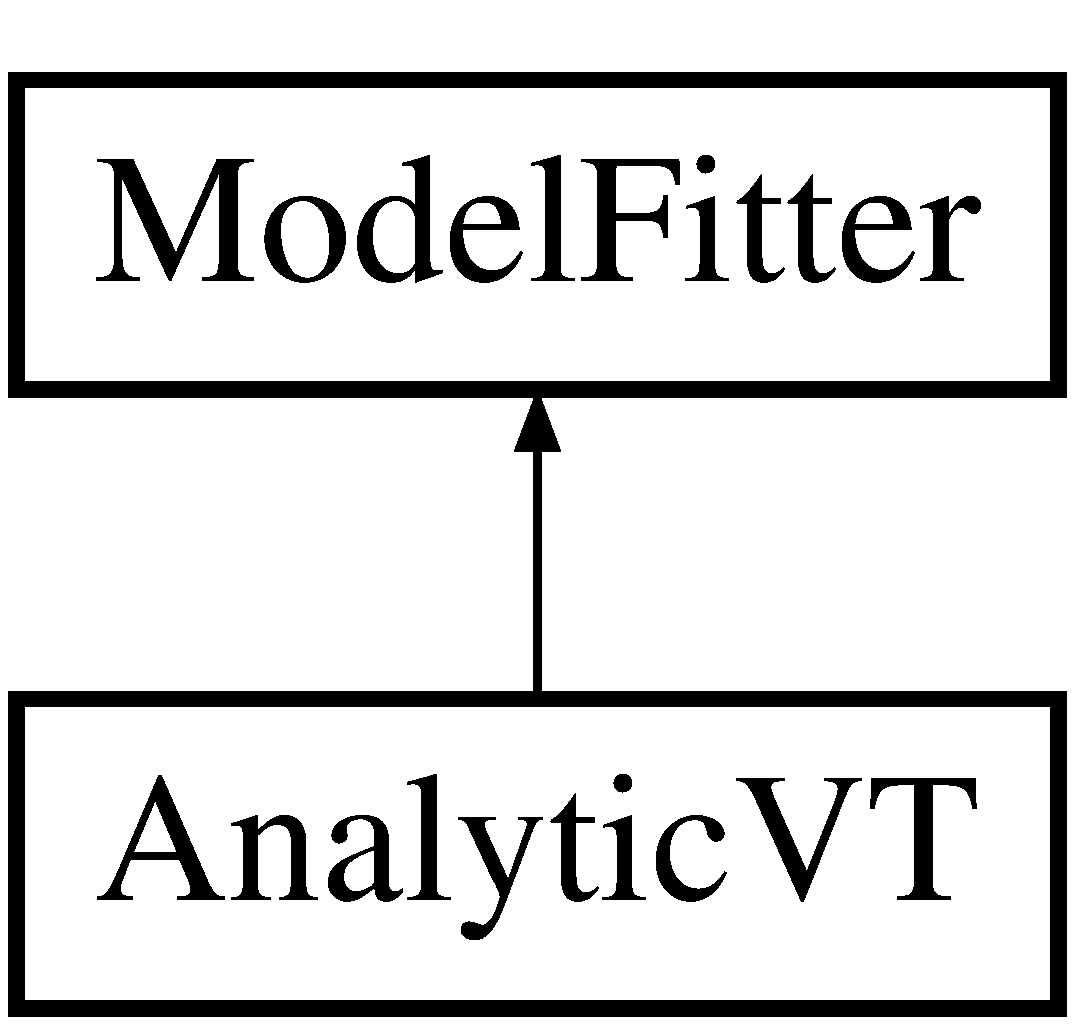
\includegraphics[height=2.000000cm]{classAnalyticVT}
\end{center}
\end{figure}
\subsection*{Public Types}
\begin{DoxyCompactItemize}
\item 
enum {\bfseries Type} \{ {\bfseries U\-N\-R\-E\-L\-A\-T\-E\-D} =  0, 
{\bfseries R\-E\-L\-A\-T\-E\-D} =  1
 \}
\end{DoxyCompactItemize}
\subsection*{Public Member Functions}
\begin{DoxyCompactItemize}
\item 
\hypertarget{classAnalyticVT_a017217a91030156c4f172d52913403f1}{{\bfseries Analytic\-V\-T} (Analytic\-V\-T\-::\-Type type)}\label{classAnalyticVT_a017217a91030156c4f172d52913403f1}

\item 
\hypertarget{classAnalyticVT_aaadf02d4c38d989c699efdef6ed35525}{int {\bfseries fit} (\hyperlink{classDataConsolidator}{Data\-Consolidator} $\ast$dc)}\label{classAnalyticVT_aaadf02d4c38d989c699efdef6ed35525}

\item 
\hypertarget{classAnalyticVT_a6c158d2a3fe417152bb96a8669be8f08}{void {\bfseries write\-Header} (File\-Writer $\ast$fp, const \hyperlink{classResult}{Result} \&site\-Info)}\label{classAnalyticVT_a6c158d2a3fe417152bb96a8669be8f08}

\item 
\hypertarget{classAnalyticVT_ab4be8f6330d5aa086bb1df11ed0f17a6}{void {\bfseries write\-Output} (File\-Writer $\ast$fp, const \hyperlink{classResult}{Result} \&site\-Info)}\label{classAnalyticVT_ab4be8f6330d5aa086bb1df11ed0f17a6}

\end{DoxyCompactItemize}
\subsection*{Additional Inherited Members}


\subsection{Detailed Description}
Implementation of variable threshold from Liu's meta-\/analysis paper 

The documentation for this class was generated from the following file\-:\begin{DoxyCompactItemize}
\item 
Model\-Fitter.\-h\end{DoxyCompactItemize}

\hypertarget{classCMATTest}{\section{C\-M\-A\-T\-Test Class Reference}
\label{classCMATTest}\index{C\-M\-A\-T\-Test@{C\-M\-A\-T\-Test}}
}
Inheritance diagram for C\-M\-A\-T\-Test\-:\begin{figure}[H]
\begin{center}
\leavevmode
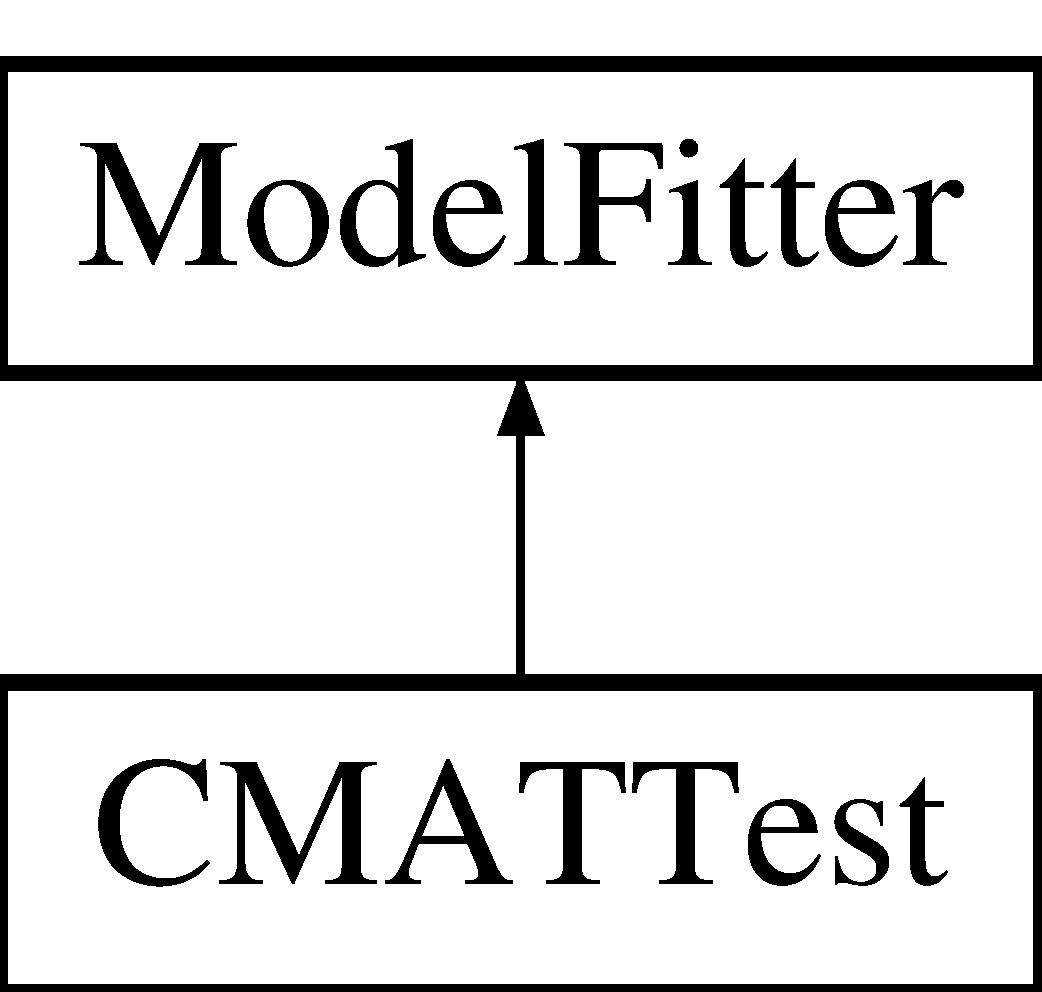
\includegraphics[height=2.000000cm]{classCMATTest}
\end{center}
\end{figure}
\subsection*{Public Member Functions}
\begin{DoxyCompactItemize}
\item 
\hypertarget{classCMATTest_a7a7de6f2ddc5efd43af959104a69e7d0}{{\bfseries C\-M\-A\-T\-Test} (int n\-Perm, double alpha)}\label{classCMATTest_a7a7de6f2ddc5efd43af959104a69e7d0}

\item 
\hypertarget{classCMATTest_a1655b4a7dfda01a1b1312e6a209e3eb8}{int {\bfseries fit} (\hyperlink{classDataConsolidator}{Data\-Consolidator} $\ast$dc)}\label{classCMATTest_a1655b4a7dfda01a1b1312e6a209e3eb8}

\item 
\hypertarget{classCMATTest_a725028ef42f405dfe485feec34ce4004}{void {\bfseries reset} ()}\label{classCMATTest_a725028ef42f405dfe485feec34ce4004}

\item 
void \hyperlink{classCMATTest_a7d11a67d555d8cb2fa21cdab61bf1f01}{write\-Header} (File\-Writer $\ast$fp, const \hyperlink{classResult}{Result} \&site\-Info)
\item 
\hypertarget{classCMATTest_a44e1f8eba1028156336ebc83900bc71f}{void {\bfseries write\-Output} (File\-Writer $\ast$fp, const \hyperlink{classResult}{Result} \&site\-Info)}\label{classCMATTest_a44e1f8eba1028156336ebc83900bc71f}

\item 
\hypertarget{classCMATTest_a66933f0ca26498ca1f4a401093102b96}{double {\bfseries calculate\-Stat} (Matrix \&genotype, Vector \&phenotype, double $\ast$p\-\_\-\-N\-\_\-\-A, double $\ast$p\-\_\-\-N\-\_\-\-U, double $\ast$p\-\_\-m\-\_\-\-A, double $\ast$p\-\_\-m\-\_\-\-U, double $\ast$p\-\_\-\-M\-\_\-\-A, double $\ast$p\-\_\-\-M\-\_\-\-U)}\label{classCMATTest_a66933f0ca26498ca1f4a401093102b96}

\end{DoxyCompactItemize}
\subsection*{Additional Inherited Members}


\subsection{Member Function Documentation}
\hypertarget{classCMATTest_a7d11a67d555d8cb2fa21cdab61bf1f01}{\index{C\-M\-A\-T\-Test@{C\-M\-A\-T\-Test}!write\-Header@{write\-Header}}
\index{write\-Header@{write\-Header}!CMATTest@{C\-M\-A\-T\-Test}}
\subsubsection[{write\-Header}]{\setlength{\rightskip}{0pt plus 5cm}void C\-M\-A\-T\-Test\-::write\-Header (
\begin{DoxyParamCaption}
\item[{File\-Writer $\ast$}]{fp, }
\item[{const {\bf Result} \&}]{site\-Info}
\end{DoxyParamCaption}
)\hspace{0.3cm}{\ttfamily [inline]}, {\ttfamily [virtual]}}}\label{classCMATTest_a7d11a67d555d8cb2fa21cdab61bf1f01}
cmat only takes binary output 

Implements \hyperlink{classModelFitter}{Model\-Fitter}.



The documentation for this class was generated from the following file\-:\begin{DoxyCompactItemize}
\item 
Model\-Fitter.\-h\end{DoxyCompactItemize}

\hypertarget{classCMCFisherExactTest}{\section{C\-M\-C\-Fisher\-Exact\-Test Class Reference}
\label{classCMCFisherExactTest}\index{C\-M\-C\-Fisher\-Exact\-Test@{C\-M\-C\-Fisher\-Exact\-Test}}
}
Inheritance diagram for C\-M\-C\-Fisher\-Exact\-Test\-:\begin{figure}[H]
\begin{center}
\leavevmode
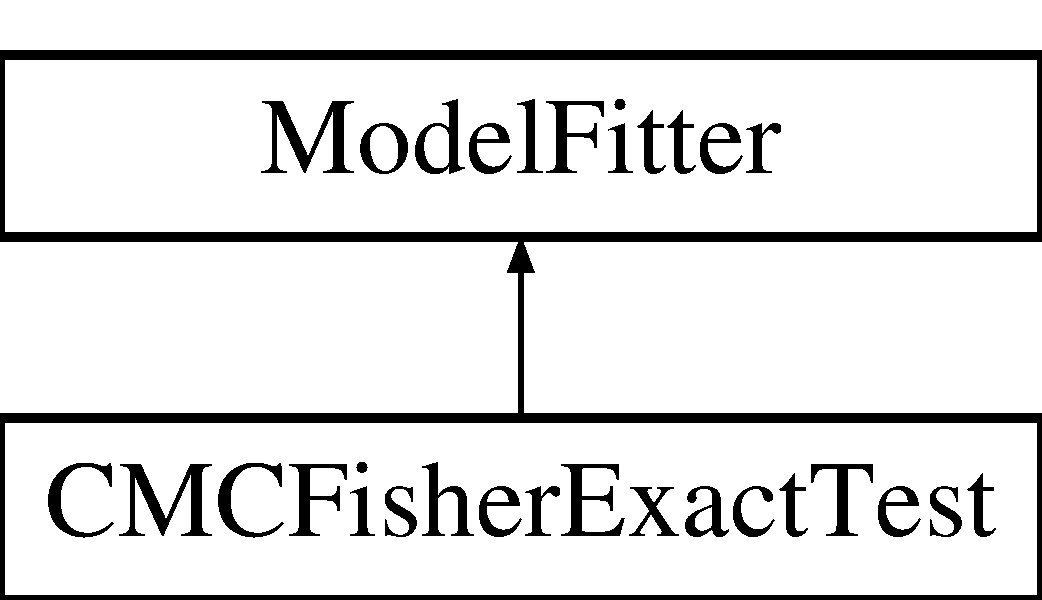
\includegraphics[height=2.000000cm]{classCMCFisherExactTest}
\end{center}
\end{figure}
\subsection*{Public Member Functions}
\begin{DoxyCompactItemize}
\item 
\hypertarget{classCMCFisherExactTest_aff85bb19c2937f8c17c0db4707919dc0}{int {\bfseries fit} (\hyperlink{classDataConsolidator}{Data\-Consolidator} $\ast$dc)}\label{classCMCFisherExactTest_aff85bb19c2937f8c17c0db4707919dc0}

\item 
\hypertarget{classCMCFisherExactTest_afc44c2bd2677c4e8de567b7b1416f396}{void {\bfseries write\-Header} (File\-Writer $\ast$fp, const \hyperlink{classResult}{Result} \&site\-Info)}\label{classCMCFisherExactTest_afc44c2bd2677c4e8de567b7b1416f396}

\item 
\hypertarget{classCMCFisherExactTest_ad50690135c2eed0f7a7b87ba4877fd17}{void {\bfseries write\-Output} (File\-Writer $\ast$fp, const \hyperlink{classResult}{Result} \&site\-Info)}\label{classCMCFisherExactTest_ad50690135c2eed0f7a7b87ba4877fd17}

\item 
\hypertarget{classCMCFisherExactTest_aea187dfb0eaf1b155d47ef3bb18b73ac}{void {\bfseries reset} ()}\label{classCMCFisherExactTest_aea187dfb0eaf1b155d47ef3bb18b73ac}

\end{DoxyCompactItemize}
\subsection*{Additional Inherited Members}


The documentation for this class was generated from the following file\-:\begin{DoxyCompactItemize}
\item 
Model\-Fitter.\-h\end{DoxyCompactItemize}

\hypertarget{classCMCTest}{\section{C\-M\-C\-Test Class Reference}
\label{classCMCTest}\index{C\-M\-C\-Test@{C\-M\-C\-Test}}
}
Inheritance diagram for C\-M\-C\-Test\-:\begin{figure}[H]
\begin{center}
\leavevmode
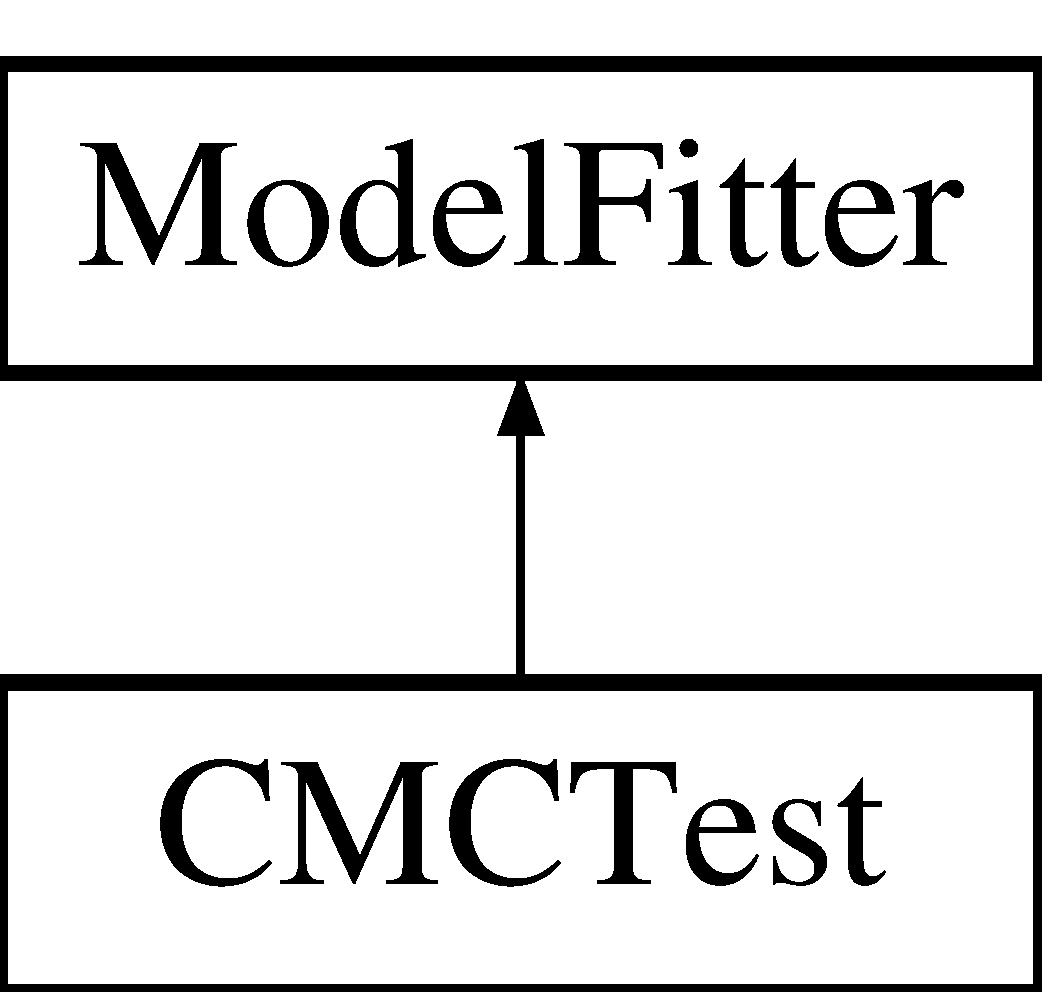
\includegraphics[height=2.000000cm]{classCMCTest}
\end{center}
\end{figure}
\subsection*{Public Member Functions}
\begin{DoxyCompactItemize}
\item 
\hypertarget{classCMCTest_a47dc595db594a6f41ae4439aca3a52fa}{int {\bfseries fit} (\hyperlink{classDataConsolidator}{Data\-Consolidator} $\ast$dc)}\label{classCMCTest_a47dc595db594a6f41ae4439aca3a52fa}

\item 
\hypertarget{classCMCTest_a97a90ee4797437bafd0465b9e41373b9}{int {\bfseries fit} (Matrix \&phenotype, Matrix \&genotype, Matrix \&covariate)}\label{classCMCTest_a97a90ee4797437bafd0465b9e41373b9}

\item 
\hypertarget{classCMCTest_a555a77c763b13a8320db7aeee772f6d0}{void {\bfseries write\-Header} (File\-Writer $\ast$fp, const \hyperlink{classResult}{Result} \&site\-Info)}\label{classCMCTest_a555a77c763b13a8320db7aeee772f6d0}

\item 
\hypertarget{classCMCTest_a82db3ff3f259352ce73774974ea00d59}{void {\bfseries write\-Output} (File\-Writer $\ast$fp, const \hyperlink{classResult}{Result} \&site\-Info)}\label{classCMCTest_a82db3ff3f259352ce73774974ea00d59}

\end{DoxyCompactItemize}
\subsection*{Additional Inherited Members}


The documentation for this class was generated from the following file\-:\begin{DoxyCompactItemize}
\item 
Model\-Fitter.\-h\end{DoxyCompactItemize}

\hypertarget{classCMCWaldTest}{\section{C\-M\-C\-Wald\-Test Class Reference}
\label{classCMCWaldTest}\index{C\-M\-C\-Wald\-Test@{C\-M\-C\-Wald\-Test}}
}
Inheritance diagram for C\-M\-C\-Wald\-Test\-:\begin{figure}[H]
\begin{center}
\leavevmode
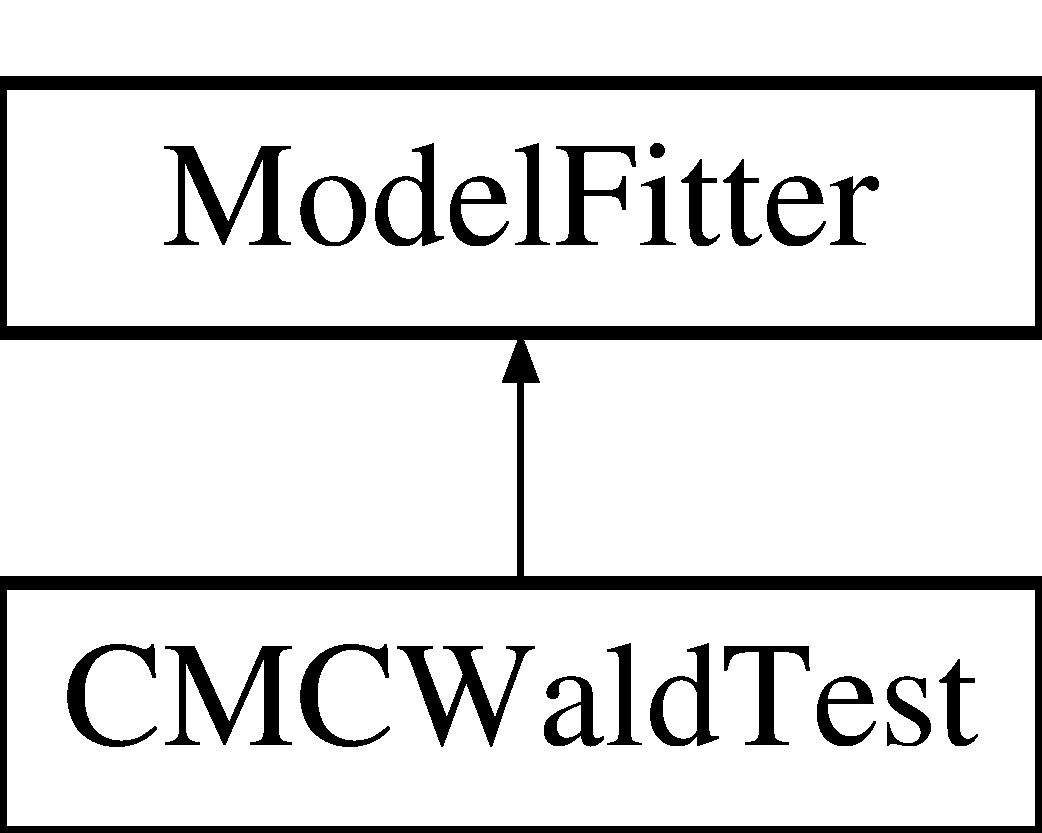
\includegraphics[height=2.000000cm]{classCMCWaldTest}
\end{center}
\end{figure}
\subsection*{Public Member Functions}
\begin{DoxyCompactItemize}
\item 
\hypertarget{classCMCWaldTest_abfa00f4336a872e6fc1354e9ba0bfe24}{int {\bfseries fit} (\hyperlink{classDataConsolidator}{Data\-Consolidator} $\ast$dc)}\label{classCMCWaldTest_abfa00f4336a872e6fc1354e9ba0bfe24}

\item 
\hypertarget{classCMCWaldTest_a2022762ee9ce5c3653b235b8041d9c4f}{void {\bfseries write\-Header} (File\-Writer $\ast$fp, const \hyperlink{classResult}{Result} \&site\-Info)}\label{classCMCWaldTest_a2022762ee9ce5c3653b235b8041d9c4f}

\item 
\hypertarget{classCMCWaldTest_a003f2de4cb62197adc9ac1de9c7741b8}{void {\bfseries write\-Output} (File\-Writer $\ast$fp, const \hyperlink{classResult}{Result} \&site\-Info)}\label{classCMCWaldTest_a003f2de4cb62197adc9ac1de9c7741b8}

\end{DoxyCompactItemize}
\subsection*{Additional Inherited Members}


The documentation for this class was generated from the following file\-:\begin{DoxyCompactItemize}
\item 
Model\-Fitter.\-h\end{DoxyCompactItemize}

\hypertarget{classCollapsor}{\section{Collapsor Class Reference}
\label{classCollapsor}\index{Collapsor@{Collapsor}}
}
\subsection*{Public Member Functions}
\begin{DoxyCompactItemize}
\item 
\hypertarget{classCollapsor_aaa7f3f52d31e81b078933fa34c57d099}{void {\bfseries set\-Set\-File\-Name} (const char $\ast$fn)}\label{classCollapsor_aaa7f3f52d31e81b078933fa34c57d099}

\item 
void \hyperlink{classCollapsor_a4215b29910ad62cb949e8b01eb0ca730}{set\-Frequency\-Cutoff} (int howto\-Calc\-Freq, double lb, double ub)
\item 
\hypertarget{classCollapsor_a833e81ad32307670e9590e921a393716}{void {\bfseries filter\-Genotype\-By\-Frequency} (\hyperlink{classVCFData}{V\-C\-F\-Data} $\ast$d)}\label{classCollapsor_a833e81ad32307670e9590e921a393716}

\item 
bool \hyperlink{classCollapsor_ac89c1d1baaf4932b80e62476e2b667e8}{iterate\-Set} (V\-C\-F\-Input\-File \&vin, \hyperlink{classVCFData}{V\-C\-F\-Data} $\ast$data)
\item 
\hypertarget{classCollapsor_a8c6f764b5b2eae1b5b5aed5b624f74b0}{std\-::string \& {\bfseries get\-Current\-Set\-Name} ()}\label{classCollapsor_a8c6f764b5b2eae1b5b5aed5b624f74b0}

\end{DoxyCompactItemize}


\subsection{Member Function Documentation}
\hypertarget{classCollapsor_ac89c1d1baaf4932b80e62476e2b667e8}{\index{Collapsor@{Collapsor}!iterate\-Set@{iterate\-Set}}
\index{iterate\-Set@{iterate\-Set}!Collapsor@{Collapsor}}
\subsubsection[{iterate\-Set}]{\setlength{\rightskip}{0pt plus 5cm}bool Collapsor\-::iterate\-Set (
\begin{DoxyParamCaption}
\item[{V\-C\-F\-Input\-File \&}]{vin, }
\item[{{\bf V\-C\-F\-Data} $\ast$}]{data}
\end{DoxyParamCaption}
)\hspace{0.3cm}{\ttfamily [inline]}}}\label{classCollapsor_ac89c1d1baaf4932b80e62476e2b667e8}
iterate all sets \begin{DoxyReturn}{Returns}
false\-: when all sets are went over 
\end{DoxyReturn}
\hypertarget{classCollapsor_a4215b29910ad62cb949e8b01eb0ca730}{\index{Collapsor@{Collapsor}!set\-Frequency\-Cutoff@{set\-Frequency\-Cutoff}}
\index{set\-Frequency\-Cutoff@{set\-Frequency\-Cutoff}!Collapsor@{Collapsor}}
\subsubsection[{set\-Frequency\-Cutoff}]{\setlength{\rightskip}{0pt plus 5cm}void Collapsor\-::set\-Frequency\-Cutoff (
\begin{DoxyParamCaption}
\item[{int}]{howto\-Calc\-Freq, }
\item[{double}]{lb, }
\item[{double}]{ub}
\end{DoxyParamCaption}
)\hspace{0.3cm}{\ttfamily [inline]}}}\label{classCollapsor_a4215b29910ad62cb949e8b01eb0ca730}

\begin{DoxyParams}{Parameters}
{\em howto\-Calc\-Freq} & freq from all sample or from all control \\
\hline
{\em lb,\-:} & lower bound \\
\hline
{\em ub,\-:} & upper bound \\
\hline
\end{DoxyParams}


The documentation for this class was generated from the following file\-:\begin{DoxyCompactItemize}
\item 
Collapsor.\-h\end{DoxyCompactItemize}

\hypertarget{classDataConsolidator}{\section{Data\-Consolidator Class Reference}
\label{classDataConsolidator}\index{Data\-Consolidator@{Data\-Consolidator}}
}


{\ttfamily \#include $<$Data\-Consolidator.\-h$>$}

\subsection*{Public Types}
\begin{DoxyCompactItemize}
\item 
enum {\bfseries P\-L\-I\-N\-K\-\_\-\-S\-E\-X} \{ {\bfseries A\-N\-Y\-\_\-\-S\-E\-X} =  -\/1, 
{\bfseries M\-A\-L\-E} =  1, 
{\bfseries F\-E\-M\-A\-L\-E} =  2
 \}
\item 
enum {\bfseries P\-L\-I\-N\-K\-\_\-\-P\-H\-E\-N\-O\-T\-Y\-P\-E} \{ {\bfseries A\-N\-Y\-\_\-\-P\-H\-E\-N\-O} =  -\/1, 
{\bfseries C\-T\-R\-L} =  1, 
{\bfseries C\-A\-S\-E} =  2
 \}
\end{DoxyCompactItemize}
\subsection*{Public Member Functions}
\begin{DoxyCompactItemize}
\item 
\hypertarget{classDataConsolidator_aaf864962320e2fa28fc345c646426d47}{void {\bfseries set\-Strategy} (const int s)}\label{classDataConsolidator_aaf864962320e2fa28fc345c646426d47}

\item 
void \hyperlink{classDataConsolidator_acc7e1257797598cb69db26dedbf909e7}{consolidate} (Matrix \&pheno, Matrix \&cov, Matrix \&geno)
\item 
\hypertarget{classDataConsolidator_a1e3186b079b05bb9484e787a1ec86288}{bool {\bfseries has\-No\-Missing\-Genotype} (Matrix \&g, int r)}\label{classDataConsolidator_a1e3186b079b05bb9484e787a1ec86288}

\item 
\hypertarget{classDataConsolidator_a486805b59a97e99bd52dfa62552b9664}{void {\bfseries copy\-Row} (Matrix \&src, const int src\-Row, Matrix $\ast$dest, const int dest\-Row)}\label{classDataConsolidator_a486805b59a97e99bd52dfa62552b9664}

\item 
\hypertarget{classDataConsolidator_ae8e8098f431f72d34065bf63c2bc72ab}{void {\bfseries copy\-Col\-Name} (Matrix \&src, Matrix $\ast$dest)}\label{classDataConsolidator_ae8e8098f431f72d34065bf63c2bc72ab}

\item 
\hypertarget{classDataConsolidator_a02f8da2a937e773627471e9c8efe0a3f}{void {\bfseries set\-Phenotype\-Name} (const std\-::vector$<$ std\-::string $>$ \&name)}\label{classDataConsolidator_a02f8da2a937e773627471e9c8efe0a3f}

\item 
\hypertarget{classDataConsolidator_a3e1b9bdaa8170965cfb48203d95fb2cb}{const std\-::vector$<$ std\-::string $>$ \& {\bfseries get\-Row\-Label} () const }\label{classDataConsolidator_a3e1b9bdaa8170965cfb48203d95fb2cb}

\item 
\hypertarget{classDataConsolidator_a07a010120f96b5e007f0437eec5a0057}{Matrix \& {\bfseries get\-Genotype} ()}\label{classDataConsolidator_a07a010120f96b5e007f0437eec5a0057}

\item 
\hypertarget{classDataConsolidator_a80a1c89b99b485c693e992bbabe88111}{Matrix \& {\bfseries get\-Phenotype} ()}\label{classDataConsolidator_a80a1c89b99b485c693e992bbabe88111}

\item 
\hypertarget{classDataConsolidator_a96c4b5b2a122e420f86714c3cb0fa451}{Matrix \& {\bfseries get\-Covariate} ()}\label{classDataConsolidator_a96c4b5b2a122e420f86714c3cb0fa451}

\item 
\hypertarget{classDataConsolidator_ab12753ca733a0bb5d15299a7e617f98e}{Vector \& {\bfseries get\-Weight} ()}\label{classDataConsolidator_ab12753ca733a0bb5d15299a7e617f98e}

\item 
\hypertarget{classDataConsolidator_a1c576cec1c21356bf5b8efb92edc610b}{\hyperlink{classResult}{Result} \& {\bfseries get\-Result} ()}\label{classDataConsolidator_a1c576cec1c21356bf5b8efb92edc610b}

\item 
int \hyperlink{classDataConsolidator_a9438e5e1cef935dc0218b6f3a224054f}{count\-Raw\-Genotype} (int column\-Index, int $\ast$hom\-Ref, int $\ast$het, int $\ast$hom\-Alt, int $\ast$missing, const P\-L\-I\-N\-K\-\_\-\-S\-E\-X sex, const P\-L\-I\-N\-K\-\_\-\-P\-H\-E\-N\-O\-T\-Y\-P\-E phenotype) const 
\item 
\hypertarget{classDataConsolidator_ade6bb3acbcf12e6cdce387c11d2665e8}{int {\bfseries count\-Raw\-Genotype\-From\-Case} (int column\-Index, int $\ast$hom\-Ref, int $\ast$het, int $\ast$hom\-Alt, int $\ast$missing) const }\label{classDataConsolidator_ade6bb3acbcf12e6cdce387c11d2665e8}

\item 
\hypertarget{classDataConsolidator_a8284e55581f7f3f9297c860732e59e00}{int {\bfseries count\-Raw\-Genotype\-From\-Control} (int column\-Index, int $\ast$hom\-Ref, int $\ast$het, int $\ast$hom\-Alt, int $\ast$missing) const }\label{classDataConsolidator_a8284e55581f7f3f9297c860732e59e00}

\item 
\hypertarget{classDataConsolidator_a8cebd4da6d55fd703b2f4b1197b494fe}{int {\bfseries count\-Raw\-Genotype} (int column\-Index, int $\ast$hom\-Ref, int $\ast$het, int $\ast$hom\-Alt, int $\ast$missing) const }\label{classDataConsolidator_a8cebd4da6d55fd703b2f4b1197b494fe}

\item 
\hypertarget{classDataConsolidator_a71dbabe3cc64f40ce1d1ee0c3d2a1ef1}{int {\bfseries count\-Raw\-Genotype\-From\-Female} (int column\-Index, int $\ast$hom\-Ref, int $\ast$het, int $\ast$hom\-Alt, int $\ast$missing) const }\label{classDataConsolidator_a71dbabe3cc64f40ce1d1ee0c3d2a1ef1}

\item 
\hypertarget{classDataConsolidator_a339b61163ca0dd39b4ca2f644593a0fc}{int {\bfseries count\-Raw\-Genotype\-From\-Female\-Case} (int column\-Index, int $\ast$hom\-Ref, int $\ast$het, int $\ast$hom\-Alt, int $\ast$missing) const }\label{classDataConsolidator_a339b61163ca0dd39b4ca2f644593a0fc}

\item 
\hypertarget{classDataConsolidator_a5b0ed490343fd48b40fe472a70f1e873}{int {\bfseries count\-Raw\-Genotype\-From\-Female\-Control} (int column\-Index, int $\ast$hom\-Ref, int $\ast$het, int $\ast$hom\-Alt, int $\ast$missing) const }\label{classDataConsolidator_a5b0ed490343fd48b40fe472a70f1e873}

\item 
\hypertarget{classDataConsolidator_ab54c06be926fc7e0bfe5026b7bd197e6}{bool {\bfseries is\-Phenotype\-Updated} () const }\label{classDataConsolidator_ab54c06be926fc7e0bfe5026b7bd197e6}

\item 
\hypertarget{classDataConsolidator_acae7e76efa22c884538b479e09d71db9}{bool {\bfseries is\-Covariate\-Updated} () const }\label{classDataConsolidator_acae7e76efa22c884538b479e09d71db9}

\item 
\hypertarget{classDataConsolidator_a86023411ac6e73487bb79d25c1b5f915}{bool {\bfseries need\-To\-Update\-Kinship} () const }\label{classDataConsolidator_a86023411ac6e73487bb79d25c1b5f915}

\item 
int \hyperlink{classDataConsolidator_af21210c0105a31392d49c1afcd1e2d78}{load\-Kinship\-File} (const std\-::string \&fn, const std\-::vector$<$ std\-::string $>$ \&names, Eigen\-Matrix $\ast$$\ast$p\-Kinship, Eigen\-Matrix $\ast$$\ast$p\-Kinship\-U, Eigen\-Matrix $\ast$$\ast$p\-Kinship\-S, bool $\ast$p\-Kinship\-Loaded)
\item 
\hypertarget{classDataConsolidator_a5a3b62e3bbbd9bf0c99e3d7da8176f8d}{int {\bfseries load\-Kinship\-File\-For\-Auto} (const std\-::string \&fn, const std\-::vector$<$ std\-::string $>$ \&names)}\label{classDataConsolidator_a5a3b62e3bbbd9bf0c99e3d7da8176f8d}

\item 
\hypertarget{classDataConsolidator_a30666fc84801cfd6e41252ba9d8838f0}{int {\bfseries load\-Kinship\-File\-For\-X} (const std\-::string \&fn, const std\-::vector$<$ std\-::string $>$ \&names)}\label{classDataConsolidator_a30666fc84801cfd6e41252ba9d8838f0}

\item 
int \hyperlink{classDataConsolidator_a296e1c33fcf7dc936de8c3c8d269aa27}{decompose\-Kinship\-For\-Auto} ()
\item 
\hypertarget{classDataConsolidator_a5f408a66bc96c5c35b46c8e037b577a4}{const Eigen\-Matrix $\ast$ {\bfseries get\-Kinship\-For\-Auto} () const }\label{classDataConsolidator_a5f408a66bc96c5c35b46c8e037b577a4}

\item 
\hypertarget{classDataConsolidator_a96264603901b05e5db06bf521e05eceb}{const Eigen\-Matrix $\ast$ {\bfseries get\-Kinship\-U\-For\-Auto} () const }\label{classDataConsolidator_a96264603901b05e5db06bf521e05eceb}

\item 
\hypertarget{classDataConsolidator_a70018150cef6a5b0286bd82104b58504}{const Eigen\-Matrix $\ast$ {\bfseries get\-Kinship\-S\-For\-Auto} () const }\label{classDataConsolidator_a70018150cef6a5b0286bd82104b58504}

\item 
\hypertarget{classDataConsolidator_ab8fc9035c1c59e9dcdaac3e1fdad15e1}{bool {\bfseries has\-Kinship\-For\-Auto} () const }\label{classDataConsolidator_ab8fc9035c1c59e9dcdaac3e1fdad15e1}

\item 
\hypertarget{classDataConsolidator_a9217cca4e2d6db91849e5b1f6cb85f7d}{int {\bfseries decompose\-Kinship\-For\-X} ()}\label{classDataConsolidator_a9217cca4e2d6db91849e5b1f6cb85f7d}

\item 
\hypertarget{classDataConsolidator_a3ad74745814e28455f21d68d9a972efe}{const Eigen\-Matrix $\ast$ {\bfseries get\-Kinship\-For\-X} () const }\label{classDataConsolidator_a3ad74745814e28455f21d68d9a972efe}

\item 
\hypertarget{classDataConsolidator_a92169c65d5e960b15f21030da2efba43}{const Eigen\-Matrix $\ast$ {\bfseries get\-Kinship\-U\-For\-X} () const }\label{classDataConsolidator_a92169c65d5e960b15f21030da2efba43}

\item 
\hypertarget{classDataConsolidator_a5c3335f177f0f9bca35199707762e43e}{const Eigen\-Matrix $\ast$ {\bfseries get\-Kinship\-S\-For\-X} () const }\label{classDataConsolidator_a5c3335f177f0f9bca35199707762e43e}

\item 
\hypertarget{classDataConsolidator_a19bf9e104900fb727863db0a1ac86406}{bool {\bfseries has\-Kinship\-For\-X} () const }\label{classDataConsolidator_a19bf9e104900fb727863db0a1ac86406}

\item 
\hypertarget{classDataConsolidator_a55c87299fae9e49cf7e56837cd9115a9}{bool {\bfseries has\-Kinship} () const }\label{classDataConsolidator_a55c87299fae9e49cf7e56837cd9115a9}

\item 
\hypertarget{classDataConsolidator_a70cead67b8c1b36c33f09abb7ecfdd4d}{void {\bfseries set\-Par\-Region} (Par\-Region $\ast$p)}\label{classDataConsolidator_a70cead67b8c1b36c33f09abb7ecfdd4d}

\item 
\hypertarget{classDataConsolidator_aa20113afd520eb2602bf474858a0e406}{void {\bfseries set\-Sex} (const std\-::vector$<$ int $>$ $\ast$sex)}\label{classDataConsolidator_aa20113afd520eb2602bf474858a0e406}

\item 
bool \hyperlink{classDataConsolidator_aff9b9fa8b9adaf51da4957585bd8d58b}{is\-Hemi\-Region} (int column\-Index)
\item 
\hypertarget{classDataConsolidator_ae1c486ce4cd359714d5b26103d30de41}{void {\bfseries code\-Genotype\-For\-Dominant\-Model} (Matrix $\ast$geno)}\label{classDataConsolidator_ae1c486ce4cd359714d5b26103d30de41}

\item 
\hypertarget{classDataConsolidator_ab2146a967d511a61c4eaec48630c0d82}{void {\bfseries code\-Genotype\-For\-Recessive\-Model} (Matrix $\ast$geno)}\label{classDataConsolidator_ab2146a967d511a61c4eaec48630c0d82}

\end{DoxyCompactItemize}
\subsection*{Static Public Attributes}
\begin{DoxyCompactItemize}
\item 
\hypertarget{classDataConsolidator_a1a79503768c029b2d3082cf018cf4c50}{static const int {\bfseries U\-N\-I\-N\-I\-T\-I\-A\-L\-I\-Z\-E\-D} = 0}\label{classDataConsolidator_a1a79503768c029b2d3082cf018cf4c50}

\item 
\hypertarget{classDataConsolidator_a96f6214f9c99bc1ce51325a654a50337}{static const int {\bfseries I\-M\-P\-U\-T\-E\-\_\-\-M\-E\-A\-N} = 1}\label{classDataConsolidator_a96f6214f9c99bc1ce51325a654a50337}

\item 
\hypertarget{classDataConsolidator_a243483b1928920c0d485add4250c29db}{static const int {\bfseries I\-M\-P\-U\-T\-E\-\_\-\-H\-W\-E} = 2}\label{classDataConsolidator_a243483b1928920c0d485add4250c29db}

\item 
\hypertarget{classDataConsolidator_aa80afbd032e7318b6adf6e91dc37b684}{static const int {\bfseries D\-R\-O\-P} = 3}\label{classDataConsolidator_aa80afbd032e7318b6adf6e91dc37b684}

\end{DoxyCompactItemize}


\subsection{Detailed Description}
This class is in charge of cleanning data before fitting in model The cleaning step includes\-: remove monomorphic sites handle missing data genotype (impute to mean, impute by H\-W\-E, or filter out mssing genotypes and its corresponding phenotypes, covariates) (future todo) include weights (G\-E\-R\-P, Sift) (future todo) re-\/weight genotype (dominate model, recessive model) 

\subsection{Member Function Documentation}
\hypertarget{classDataConsolidator_acc7e1257797598cb69db26dedbf909e7}{\index{Data\-Consolidator@{Data\-Consolidator}!consolidate@{consolidate}}
\index{consolidate@{consolidate}!DataConsolidator@{Data\-Consolidator}}
\subsubsection[{consolidate}]{\setlength{\rightskip}{0pt plus 5cm}void Data\-Consolidator\-::consolidate (
\begin{DoxyParamCaption}
\item[{Matrix \&}]{pheno, }
\item[{Matrix \&}]{cov, }
\item[{Matrix \&}]{geno}
\end{DoxyParamCaption}
)\hspace{0.3cm}{\ttfamily [inline]}}}\label{classDataConsolidator_acc7e1257797598cb69db26dedbf909e7}

\begin{DoxyParams}{Parameters}
{\em pheno,@param} & cov \\
\hline
{\em genotype} & are all ordered and sorted by the same people \\
\hline
{\em pheno\-Out,@param} & cov\-Out and \\
\hline
{\em genotype} & are outputted N\-O\-T\-E\-: \\
\hline
{\em cov\-Out} & may be filled as column vector of 1 if \\
\hline
{\em cov} & is empty \\
\hline
\end{DoxyParams}
\hypertarget{classDataConsolidator_a9438e5e1cef935dc0218b6f3a224054f}{\index{Data\-Consolidator@{Data\-Consolidator}!count\-Raw\-Genotype@{count\-Raw\-Genotype}}
\index{count\-Raw\-Genotype@{count\-Raw\-Genotype}!DataConsolidator@{Data\-Consolidator}}
\subsubsection[{count\-Raw\-Genotype}]{\setlength{\rightskip}{0pt plus 5cm}int Data\-Consolidator\-::count\-Raw\-Genotype (
\begin{DoxyParamCaption}
\item[{int}]{column\-Index, }
\item[{int $\ast$}]{hom\-Ref, }
\item[{int $\ast$}]{het, }
\item[{int $\ast$}]{hom\-Alt, }
\item[{int $\ast$}]{missing, }
\item[{const P\-L\-I\-N\-K\-\_\-\-S\-E\-X}]{sex, }
\item[{const P\-L\-I\-N\-K\-\_\-\-P\-H\-E\-N\-O\-T\-Y\-P\-E}]{phenotype}
\end{DoxyParamCaption}
) const\hspace{0.3cm}{\ttfamily [inline]}}}\label{classDataConsolidator_a9438e5e1cef935dc0218b6f3a224054f}
Count 
\begin{DoxyParams}{Parameters}
{\em hom\-Ref,@param} & het, \\
\hline
{\em hom\-Alt} & and \\
\hline
{\em missing} & from the genotype column specified by \\
\hline
{\em column\-Index} & \\
\hline
{\em sex} & \-: only process specified sex (1, male; 2, female; $<$0, any) \\
\hline
{\em phenotype,\-:} & only process specified phenotype (1, control; 2, case; $<$0 any) \\
\hline
\end{DoxyParams}
\begin{DoxyReturn}{Returns}
0 if succeed 
\end{DoxyReturn}
\hypertarget{classDataConsolidator_a296e1c33fcf7dc936de8c3c8d269aa27}{\index{Data\-Consolidator@{Data\-Consolidator}!decompose\-Kinship\-For\-Auto@{decompose\-Kinship\-For\-Auto}}
\index{decompose\-Kinship\-For\-Auto@{decompose\-Kinship\-For\-Auto}!DataConsolidator@{Data\-Consolidator}}
\subsubsection[{decompose\-Kinship\-For\-Auto}]{\setlength{\rightskip}{0pt plus 5cm}int Data\-Consolidator\-::decompose\-Kinship\-For\-Auto (
\begin{DoxyParamCaption}
{}
\end{DoxyParamCaption}
)}}\label{classDataConsolidator_a296e1c33fcf7dc936de8c3c8d269aa27}
will decompose original kinship matrix and release the memory of original kinship upon successful decomposition Kinship = U $\ast$ S $\ast$ U' where S is diagonal matrix from smallest to largest

Decompose autosomal kinship matrix and release its memory K = U $\ast$ S $\ast$ U' \begin{DoxyReturn}{Returns}
0 if success 
\end{DoxyReturn}
\hypertarget{classDataConsolidator_aff9b9fa8b9adaf51da4957585bd8d58b}{\index{Data\-Consolidator@{Data\-Consolidator}!is\-Hemi\-Region@{is\-Hemi\-Region}}
\index{is\-Hemi\-Region@{is\-Hemi\-Region}!DataConsolidator@{Data\-Consolidator}}
\subsubsection[{is\-Hemi\-Region}]{\setlength{\rightskip}{0pt plus 5cm}bool Data\-Consolidator\-::is\-Hemi\-Region (
\begin{DoxyParamCaption}
\item[{int}]{column\-Index}
\end{DoxyParamCaption}
)\hspace{0.3cm}{\ttfamily [inline]}}}\label{classDataConsolidator_aff9b9fa8b9adaf51da4957585bd8d58b}
Check if genotype matrix column 
\begin{DoxyParams}{Parameters}
{\em column\-Index} & is a chromosome X. \\
\hline
\end{DoxyParams}
\hypertarget{classDataConsolidator_af21210c0105a31392d49c1afcd1e2d78}{\index{Data\-Consolidator@{Data\-Consolidator}!load\-Kinship\-File@{load\-Kinship\-File}}
\index{load\-Kinship\-File@{load\-Kinship\-File}!DataConsolidator@{Data\-Consolidator}}
\subsubsection[{load\-Kinship\-File}]{\setlength{\rightskip}{0pt plus 5cm}int Data\-Consolidator\-::load\-Kinship\-File (
\begin{DoxyParamCaption}
\item[{const std\-::string \&}]{fn, }
\item[{const std\-::vector$<$ std\-::string $>$ \&}]{names, }
\item[{Eigen\-Matrix $\ast$$\ast$}]{p\-Kinship, }
\item[{Eigen\-Matrix $\ast$$\ast$}]{p\-Kinship\-U, }
\item[{Eigen\-Matrix $\ast$$\ast$}]{p\-Kinship\-S, }
\item[{bool $\ast$}]{p\-Kinship\-Loaded}
\end{DoxyParamCaption}
)}}\label{classDataConsolidator_af21210c0105a31392d49c1afcd1e2d78}
Load kinship file 
\begin{DoxyParams}{Parameters}
{\em fn,load} & samples given by \\
\hline
{\em names} & Store results to \\
\hline
{\em p\-Kinship,@param} & p\-Kinship\-U, \\
\hline
{\em p\-Kinship\-S} & \\
\hline
\end{DoxyParams}


The documentation for this class was generated from the following files\-:\begin{DoxyCompactItemize}
\item 
Data\-Consolidator.\-h\item 
Data\-Consolidator.\-cpp\end{DoxyCompactItemize}

\hypertarget{classDumpModel}{\section{Dump\-Model Class Reference}
\label{classDumpModel}\index{Dump\-Model@{Dump\-Model}}
}
Inheritance diagram for Dump\-Model\-:\begin{figure}[H]
\begin{center}
\leavevmode
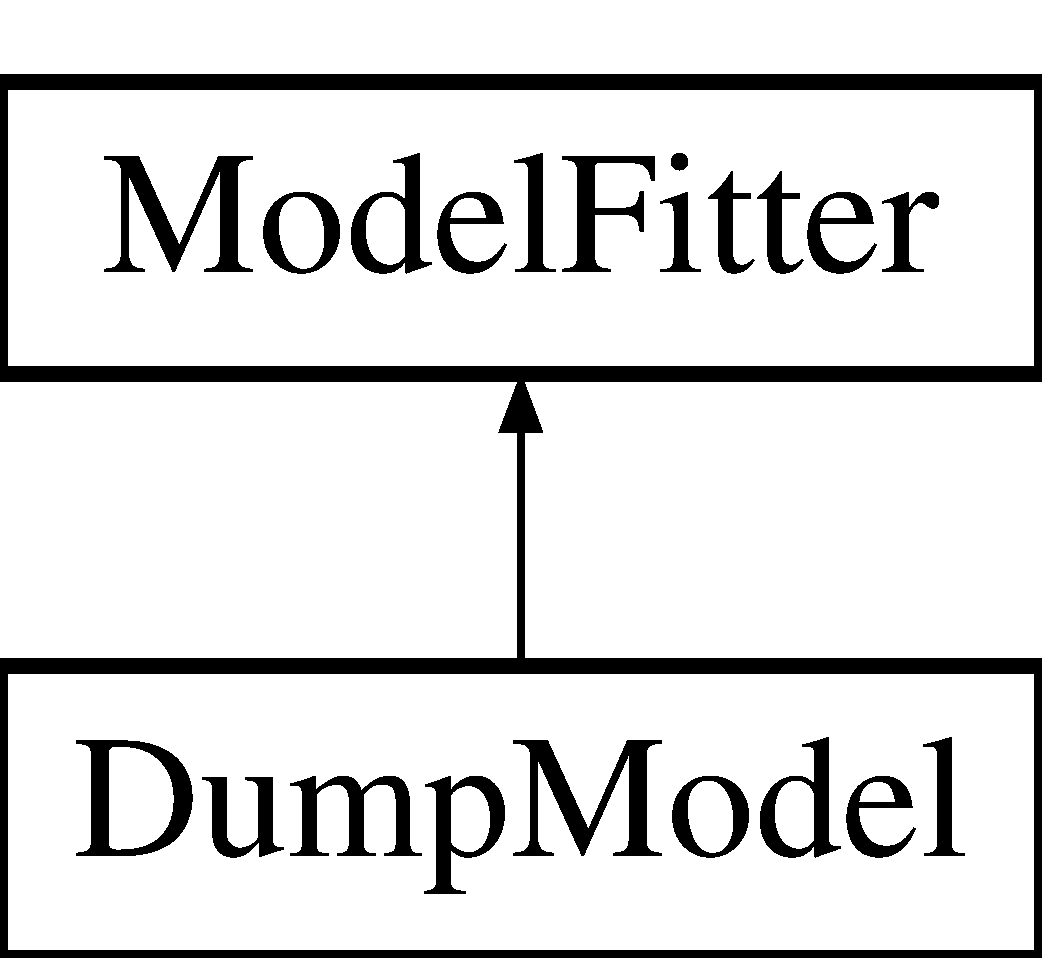
\includegraphics[height=2.000000cm]{classDumpModel}
\end{center}
\end{figure}
\subsection*{Public Member Functions}
\begin{DoxyCompactItemize}
\item 
\hypertarget{classDumpModel_adc586e8f306f77d6a7b461b034f1c26d}{{\bfseries Dump\-Model} (const char $\ast$prefix)}\label{classDumpModel_adc586e8f306f77d6a7b461b034f1c26d}

\item 
\hypertarget{classDumpModel_abdb9111db3a72c3ea52f99a7fd3cdaa3}{void {\bfseries write\-Header} (File\-Writer $\ast$fp, const \hyperlink{classResult}{Result} \&site\-Info)}\label{classDumpModel_abdb9111db3a72c3ea52f99a7fd3cdaa3}

\item 
\hypertarget{classDumpModel_a97c88e2942815e95bdb924f88c6083a4}{int {\bfseries fit} (\hyperlink{classDataConsolidator}{Data\-Consolidator} $\ast$dc)}\label{classDumpModel_a97c88e2942815e95bdb924f88c6083a4}

\item 
\hypertarget{classDumpModel_a3d0a2e4ff56b28e167d5c2d554640917}{void {\bfseries write\-Output} (File\-Writer $\ast$fp, const \hyperlink{classResult}{Result} \&site\-Info)}\label{classDumpModel_a3d0a2e4ff56b28e167d5c2d554640917}

\item 
\hypertarget{classDumpModel_adad74c4ddd06bb4d246bb9695b625ce7}{void {\bfseries reset} ()}\label{classDumpModel_adad74c4ddd06bb4d246bb9695b625ce7}

\end{DoxyCompactItemize}
\subsection*{Additional Inherited Members}


The documentation for this class was generated from the following file\-:\begin{DoxyCompactItemize}
\item 
Model\-Fitter.\-h\end{DoxyCompactItemize}

\hypertarget{classFamCMC}{\section{Fam\-C\-M\-C Class Reference}
\label{classFamCMC}\index{Fam\-C\-M\-C@{Fam\-C\-M\-C}}
}
Inheritance diagram for Fam\-C\-M\-C\-:\begin{figure}[H]
\begin{center}
\leavevmode
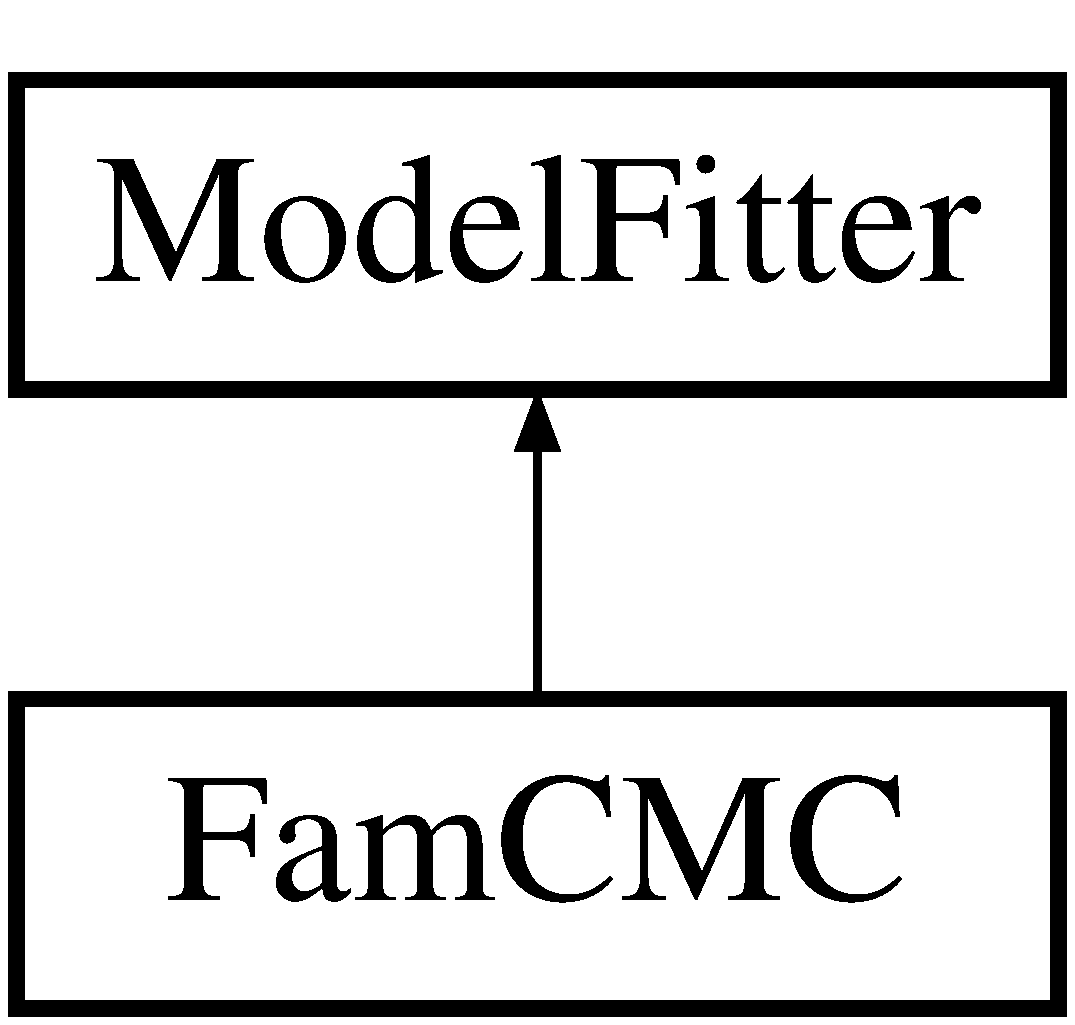
\includegraphics[height=2.000000cm]{classFamCMC}
\end{center}
\end{figure}
\subsection*{Public Member Functions}
\begin{DoxyCompactItemize}
\item 
\hypertarget{classFamCMC_af0998c134d876c1f64170b1fe7dea080}{int {\bfseries fit} (\hyperlink{classDataConsolidator}{Data\-Consolidator} $\ast$dc)}\label{classFamCMC_af0998c134d876c1f64170b1fe7dea080}

\item 
\hypertarget{classFamCMC_a017101c6c6a0bb525a392fb3b20399cf}{void {\bfseries write\-Header} (File\-Writer $\ast$fp, const \hyperlink{classResult}{Result} \&site\-Info)}\label{classFamCMC_a017101c6c6a0bb525a392fb3b20399cf}

\item 
\hypertarget{classFamCMC_a2faed912df51ba93547a99ee6e3b56d7}{void {\bfseries write\-Output} (File\-Writer $\ast$fp, const \hyperlink{classResult}{Result} \&site\-Info)}\label{classFamCMC_a2faed912df51ba93547a99ee6e3b56d7}

\item 
\hypertarget{classFamCMC_af373263e19607d74dde498b210651dbf}{void {\bfseries write\-Footnote} (File\-Writer $\ast$fp)}\label{classFamCMC_af373263e19607d74dde498b210651dbf}

\end{DoxyCompactItemize}
\subsection*{Additional Inherited Members}


The documentation for this class was generated from the following file\-:\begin{DoxyCompactItemize}
\item 
Model\-Fitter.\-h\end{DoxyCompactItemize}

\hypertarget{classFamSkatTest}{\section{Fam\-Skat\-Test Class Reference}
\label{classFamSkatTest}\index{Fam\-Skat\-Test@{Fam\-Skat\-Test}}
}
Inheritance diagram for Fam\-Skat\-Test\-:\begin{figure}[H]
\begin{center}
\leavevmode
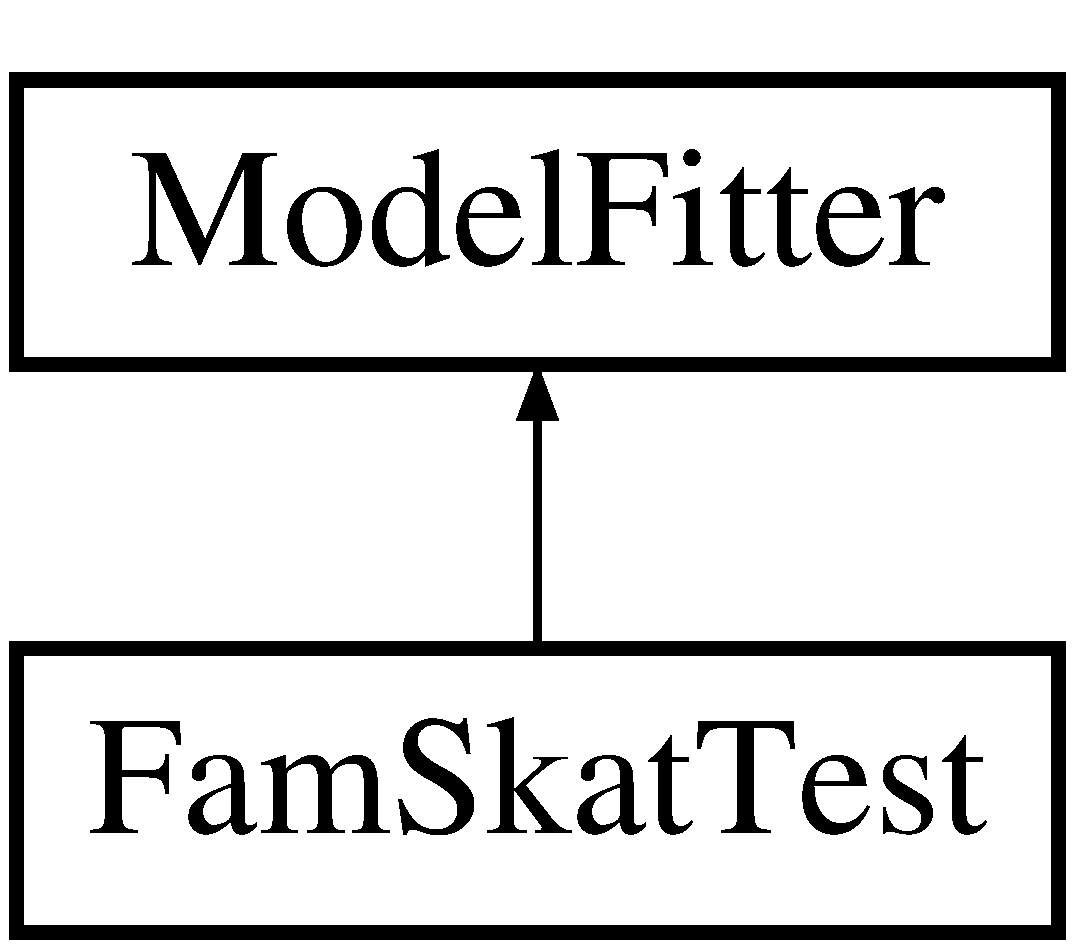
\includegraphics[height=2.000000cm]{classFamSkatTest}
\end{center}
\end{figure}
\subsection*{Public Member Functions}
\begin{DoxyCompactItemize}
\item 
\hypertarget{classFamSkatTest_a68834491a02d63ccfcaf93e842f0df51}{{\bfseries Fam\-Skat\-Test} (double beta1, double beta2)}\label{classFamSkatTest_a68834491a02d63ccfcaf93e842f0df51}

\item 
\hypertarget{classFamSkatTest_af01c84ca854dda403f83b90b5f331bc0}{int {\bfseries fit} (\hyperlink{classDataConsolidator}{Data\-Consolidator} $\ast$dc)}\label{classFamSkatTest_af01c84ca854dda403f83b90b5f331bc0}

\item 
\hypertarget{classFamSkatTest_af99548cd85658b926faab311a06fbf04}{void {\bfseries write\-Header} (File\-Writer $\ast$fp, const \hyperlink{classResult}{Result} \&site\-Info)}\label{classFamSkatTest_af99548cd85658b926faab311a06fbf04}

\item 
\hypertarget{classFamSkatTest_a067b0308aff8b331c8d2c8a08d0c6f5e}{void {\bfseries write\-Output} (File\-Writer $\ast$fp, const \hyperlink{classResult}{Result} \&site\-Info)}\label{classFamSkatTest_a067b0308aff8b331c8d2c8a08d0c6f5e}

\end{DoxyCompactItemize}
\subsection*{Additional Inherited Members}


The documentation for this class was generated from the following file\-:\begin{DoxyCompactItemize}
\item 
Model\-Fitter.\-h\end{DoxyCompactItemize}

\hypertarget{classFamZeggini}{\section{Fam\-Zeggini Class Reference}
\label{classFamZeggini}\index{Fam\-Zeggini@{Fam\-Zeggini}}
}
Inheritance diagram for Fam\-Zeggini\-:\begin{figure}[H]
\begin{center}
\leavevmode
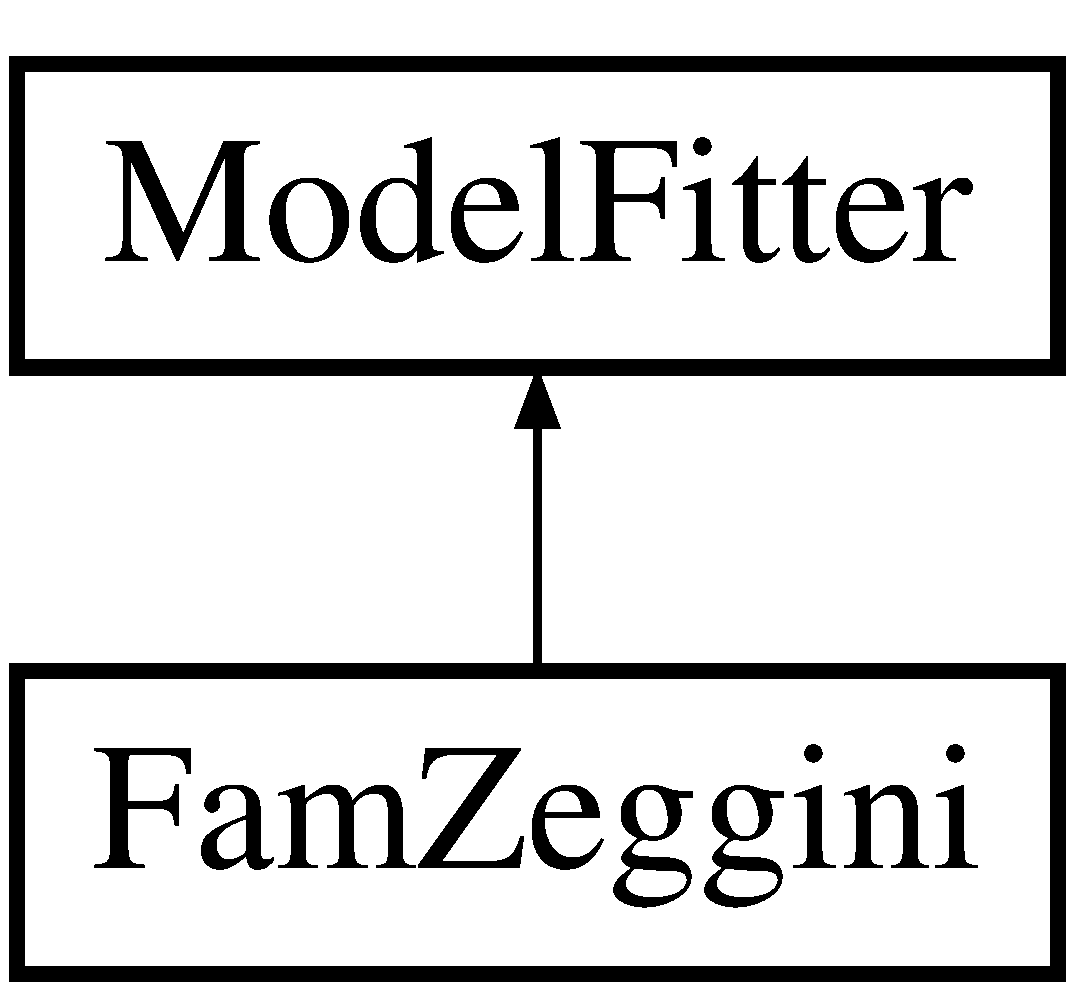
\includegraphics[height=2.000000cm]{classFamZeggini}
\end{center}
\end{figure}
\subsection*{Public Member Functions}
\begin{DoxyCompactItemize}
\item 
\hypertarget{classFamZeggini_a4f0fbfa487090e49b64a12eba230a6e9}{int {\bfseries fit} (\hyperlink{classDataConsolidator}{Data\-Consolidator} $\ast$dc)}\label{classFamZeggini_a4f0fbfa487090e49b64a12eba230a6e9}

\item 
\hypertarget{classFamZeggini_a7c8a30983804f47b57d5ffc56a9b3c83}{void {\bfseries write\-Header} (File\-Writer $\ast$fp, const \hyperlink{classResult}{Result} \&site\-Info)}\label{classFamZeggini_a7c8a30983804f47b57d5ffc56a9b3c83}

\item 
\hypertarget{classFamZeggini_a6b4ed053d08481446ad7f6a806320d88}{void {\bfseries write\-Output} (File\-Writer $\ast$fp, const \hyperlink{classResult}{Result} \&site\-Info)}\label{classFamZeggini_a6b4ed053d08481446ad7f6a806320d88}

\item 
\hypertarget{classFamZeggini_a9158d6830c268d5117ccec85e44c8118}{void {\bfseries write\-Footnote} (File\-Writer $\ast$fp)}\label{classFamZeggini_a9158d6830c268d5117ccec85e44c8118}

\end{DoxyCompactItemize}
\subsection*{Additional Inherited Members}


The documentation for this class was generated from the following file\-:\begin{DoxyCompactItemize}
\item 
Model\-Fitter.\-h\end{DoxyCompactItemize}

\hypertarget{classFpTest}{\section{Fp\-Test Class Reference}
\label{classFpTest}\index{Fp\-Test@{Fp\-Test}}
}
Inheritance diagram for Fp\-Test\-:\begin{figure}[H]
\begin{center}
\leavevmode
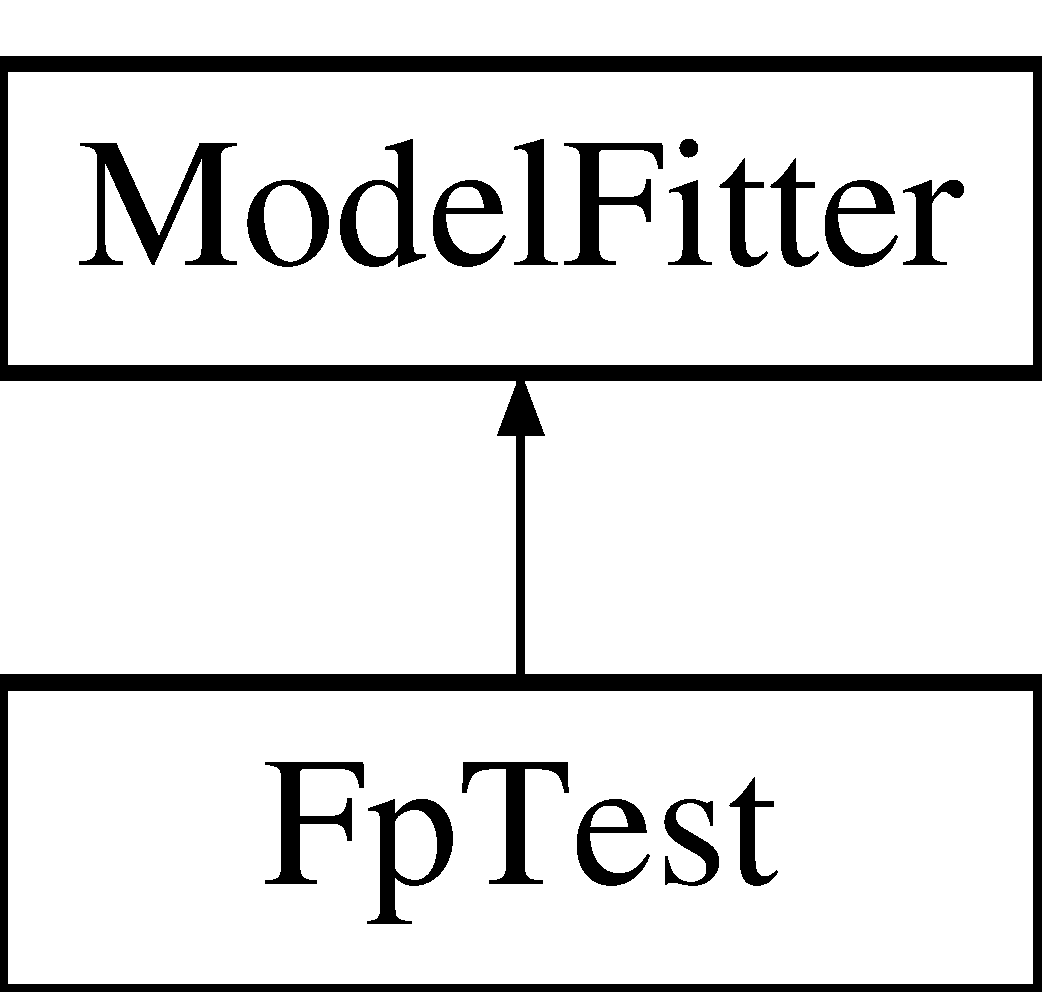
\includegraphics[height=2.000000cm]{classFpTest}
\end{center}
\end{figure}
\subsection*{Public Member Functions}
\begin{DoxyCompactItemize}
\item 
\hypertarget{classFpTest_ab655e9538e35ed22245a30f49ace14b4}{int {\bfseries fit} (\hyperlink{classDataConsolidator}{Data\-Consolidator} $\ast$dc)}\label{classFpTest_ab655e9538e35ed22245a30f49ace14b4}

\item 
\hypertarget{classFpTest_a6139c4ef019c267eda9a5fc8baabb3c6}{void {\bfseries write\-Header} (File\-Writer $\ast$fp, const \hyperlink{classResult}{Result} \&site\-Info)}\label{classFpTest_a6139c4ef019c267eda9a5fc8baabb3c6}

\item 
\hypertarget{classFpTest_a7bc54d5ccb09f8e8858717c8f57abfa4}{void {\bfseries write\-Output} (File\-Writer $\ast$fp, const \hyperlink{classResult}{Result} \&site\-Info)}\label{classFpTest_a7bc54d5ccb09f8e8858717c8f57abfa4}

\end{DoxyCompactItemize}
\subsection*{Additional Inherited Members}


The documentation for this class was generated from the following file\-:\begin{DoxyCompactItemize}
\item 
Model\-Fitter.\-h\end{DoxyCompactItemize}

\hypertarget{classGenotypeExtractor}{\section{Genotype\-Extractor Class Reference}
\label{classGenotypeExtractor}\index{Genotype\-Extractor@{Genotype\-Extractor}}
}
\subsection*{Public Member Functions}
\begin{DoxyCompactItemize}
\item 
\hypertarget{classGenotypeExtractor_a6ff59c48d46fed9aa928d90bf7500e39}{{\bfseries Genotype\-Extractor} (V\-C\-F\-Extractor $\ast$v)}\label{classGenotypeExtractor_a6ff59c48d46fed9aa928d90bf7500e39}

\item 
int \hyperlink{classGenotypeExtractor_a404348b817a6844d0a88983cb46c326c}{extract\-Multiple\-Genotype} (Matrix $\ast$g)
\item 
int \hyperlink{classGenotypeExtractor_a84d6e7394ece8f32ffcc08377a1db30e}{extract\-Single\-Genotype} (Matrix $\ast$g, \hyperlink{classResult}{Result} $\ast$b)
\item 
\hypertarget{classGenotypeExtractor_aef7a95ffb96b9ad7ce1f4cc4858fbc22}{bool {\bfseries set\-Site\-Freq\-Min} (const double f)}\label{classGenotypeExtractor_aef7a95ffb96b9ad7ce1f4cc4858fbc22}

\item 
\hypertarget{classGenotypeExtractor_a0777da1c25ac6388d0c110827bb92b8b}{bool {\bfseries set\-Site\-Freq\-Max} (const double f)}\label{classGenotypeExtractor_a0777da1c25ac6388d0c110827bb92b8b}

\item 
\hypertarget{classGenotypeExtractor_aa4708bbdd89f464b67eb4be1dd8bfad3}{bool {\bfseries check\-G\-D} (V\-C\-F\-Individual $\ast$indv, int gd\-Idx)}\label{classGenotypeExtractor_aa4708bbdd89f464b67eb4be1dd8bfad3}

\item 
\hypertarget{classGenotypeExtractor_ae93e2c35f08df71764cae8921dd5019d}{bool {\bfseries check\-G\-Q} (V\-C\-F\-Individual $\ast$indv, int gq\-Idx)}\label{classGenotypeExtractor_ae93e2c35f08df71764cae8921dd5019d}

\item 
\hypertarget{classGenotypeExtractor_a2f98e3e13638f430362d0b8099c379d2}{void {\bfseries set\-G\-Dmin} (int m)}\label{classGenotypeExtractor_a2f98e3e13638f430362d0b8099c379d2}

\item 
\hypertarget{classGenotypeExtractor_aebb1afb9de7eee2cd62da0bfbf3bba7c}{void {\bfseries set\-G\-Dmax} (int m)}\label{classGenotypeExtractor_aebb1afb9de7eee2cd62da0bfbf3bba7c}

\item 
\hypertarget{classGenotypeExtractor_a27ff068f92acf500eb07f3b4ad9e7aea}{void {\bfseries set\-G\-Qmin} (int m)}\label{classGenotypeExtractor_a27ff068f92acf500eb07f3b4ad9e7aea}

\item 
\hypertarget{classGenotypeExtractor_ade3ad5e5dfc254ef22e3692f7ac00c67}{void {\bfseries set\-G\-Qmax} (int m)}\label{classGenotypeExtractor_ade3ad5e5dfc254ef22e3692f7ac00c67}

\item 
Vector \& \hyperlink{classGenotypeExtractor_ab924228dcf705f329804acebca1df812}{get\-Weight} ()
\item 
\hypertarget{classGenotypeExtractor_ab488139105b763cb4ee6c29c95ea8893}{void {\bfseries set\-Dosage\-Tag} (const std\-::string \&tag)}\label{classGenotypeExtractor_ab488139105b763cb4ee6c29c95ea8893}

\item 
\hypertarget{classGenotypeExtractor_ab9962575d690cff556bc62d350079321}{void {\bfseries unset\-Dosage\-Tag} ()}\label{classGenotypeExtractor_ab9962575d690cff556bc62d350079321}

\item 
\hypertarget{classGenotypeExtractor_aeb13746f85a90205c694095bb39d3270}{void {\bfseries set\-Par\-Region} (Par\-Region $\ast$p)}\label{classGenotypeExtractor_aeb13746f85a90205c694095bb39d3270}

\item 
\hypertarget{classGenotypeExtractor_aca852e602aedb79687feb339db55f741}{void {\bfseries set\-Sex} (const std\-::vector$<$ int $>$ $\ast$sex)}\label{classGenotypeExtractor_aca852e602aedb79687feb339db55f741}

\item 
\hypertarget{classGenotypeExtractor_a869c1288481f87a22d150f7dcb660ab3}{void {\bfseries enable\-Clayton\-Coding} ()}\label{classGenotypeExtractor_a869c1288481f87a22d150f7dcb660ab3}

\item 
\hypertarget{classGenotypeExtractor_ac8490f1cee6ace4d9a32e99d8a06b935}{void {\bfseries disable\-Clayton\-Coding} ()}\label{classGenotypeExtractor_ac8490f1cee6ace4d9a32e99d8a06b935}

\end{DoxyCompactItemize}
\subsection*{Static Public Attributes}
\begin{DoxyCompactItemize}
\item 
\hypertarget{classGenotypeExtractor_a235fd507d4129618852329645c6fa4d7}{static const int {\bfseries S\-U\-C\-C\-E\-E\-D} = 0}\label{classGenotypeExtractor_a235fd507d4129618852329645c6fa4d7}

\item 
\hypertarget{classGenotypeExtractor_aa40d806a23dfadfb81cc2dcb247aef73}{static const int {\bfseries E\-R\-R\-O\-R} = -\/1}\label{classGenotypeExtractor_aa40d806a23dfadfb81cc2dcb247aef73}

\item 
\hypertarget{classGenotypeExtractor_a7a0e5852bc6da31847be2bbcecab56c0}{static const int {\bfseries F\-I\-L\-E\-\_\-\-E\-N\-D} = -\/2}\label{classGenotypeExtractor_a7a0e5852bc6da31847be2bbcecab56c0}

\item 
\hypertarget{classGenotypeExtractor_ae1ed6e49b539071e6d13e1745d0cc1b0}{static const int {\bfseries F\-A\-I\-L\-\_\-\-F\-I\-L\-T\-E\-R} = -\/3}\label{classGenotypeExtractor_ae1ed6e49b539071e6d13e1745d0cc1b0}

\end{DoxyCompactItemize}


\subsection{Member Function Documentation}
\hypertarget{classGenotypeExtractor_a404348b817a6844d0a88983cb46c326c}{\index{Genotype\-Extractor@{Genotype\-Extractor}!extract\-Multiple\-Genotype@{extract\-Multiple\-Genotype}}
\index{extract\-Multiple\-Genotype@{extract\-Multiple\-Genotype}!GenotypeExtractor@{Genotype\-Extractor}}
\subsubsection[{extract\-Multiple\-Genotype}]{\setlength{\rightskip}{0pt plus 5cm}int Genotype\-Extractor\-::extract\-Multiple\-Genotype (
\begin{DoxyParamCaption}
\item[{Matrix $\ast$}]{g}
\end{DoxyParamCaption}
)\hspace{0.3cm}{\ttfamily [inline]}}}\label{classGenotypeExtractor_a404348b817a6844d0a88983cb46c326c}

\begin{DoxyParams}{Parameters}
{\em g,store} & people by marker matrix \\
\hline
\end{DoxyParams}
\begin{DoxyReturn}{Returns}
0 for success 
\end{DoxyReturn}
\hypertarget{classGenotypeExtractor_a84d6e7394ece8f32ffcc08377a1db30e}{\index{Genotype\-Extractor@{Genotype\-Extractor}!extract\-Single\-Genotype@{extract\-Single\-Genotype}}
\index{extract\-Single\-Genotype@{extract\-Single\-Genotype}!GenotypeExtractor@{Genotype\-Extractor}}
\subsubsection[{extract\-Single\-Genotype}]{\setlength{\rightskip}{0pt plus 5cm}int Genotype\-Extractor\-::extract\-Single\-Genotype (
\begin{DoxyParamCaption}
\item[{Matrix $\ast$}]{g, }
\item[{{\bf Result} $\ast$}]{b}
\end{DoxyParamCaption}
)\hspace{0.3cm}{\ttfamily [inline]}}}\label{classGenotypeExtractor_a84d6e7394ece8f32ffcc08377a1db30e}
\begin{DoxyReturn}{Returns}
0 for success 

-\/2 for reach end. 
\end{DoxyReturn}

\begin{DoxyParams}{Parameters}
{\em g,\-:} & people by 1 matrix, where column name is like \char`\"{}chr\-:pos\char`\"{} \\
\hline
{\em b,\-:} & extract information, e.\-g. \char`\"{}1\textbackslash{}t100\textbackslash{}t\-A\textbackslash{}t\-C\char`\"{} \\
\hline
\end{DoxyParams}
\hypertarget{classGenotypeExtractor_ab924228dcf705f329804acebca1df812}{\index{Genotype\-Extractor@{Genotype\-Extractor}!get\-Weight@{get\-Weight}}
\index{get\-Weight@{get\-Weight}!GenotypeExtractor@{Genotype\-Extractor}}
\subsubsection[{get\-Weight}]{\setlength{\rightskip}{0pt plus 5cm}Vector\& Genotype\-Extractor\-::get\-Weight (
\begin{DoxyParamCaption}
{}
\end{DoxyParamCaption}
)\hspace{0.3cm}{\ttfamily [inline]}}}\label{classGenotypeExtractor_ab924228dcf705f329804acebca1df812}
\begin{DoxyReturn}{Returns}
weigth, its length equals to \# of markers 
\end{DoxyReturn}


The documentation for this class was generated from the following file\-:\begin{DoxyCompactItemize}
\item 
Main.\-cpp\end{DoxyCompactItemize}

\hypertarget{classKBACTest}{\section{K\-B\-A\-C\-Test Class Reference}
\label{classKBACTest}\index{K\-B\-A\-C\-Test@{K\-B\-A\-C\-Test}}
}
Inheritance diagram for K\-B\-A\-C\-Test\-:\begin{figure}[H]
\begin{center}
\leavevmode
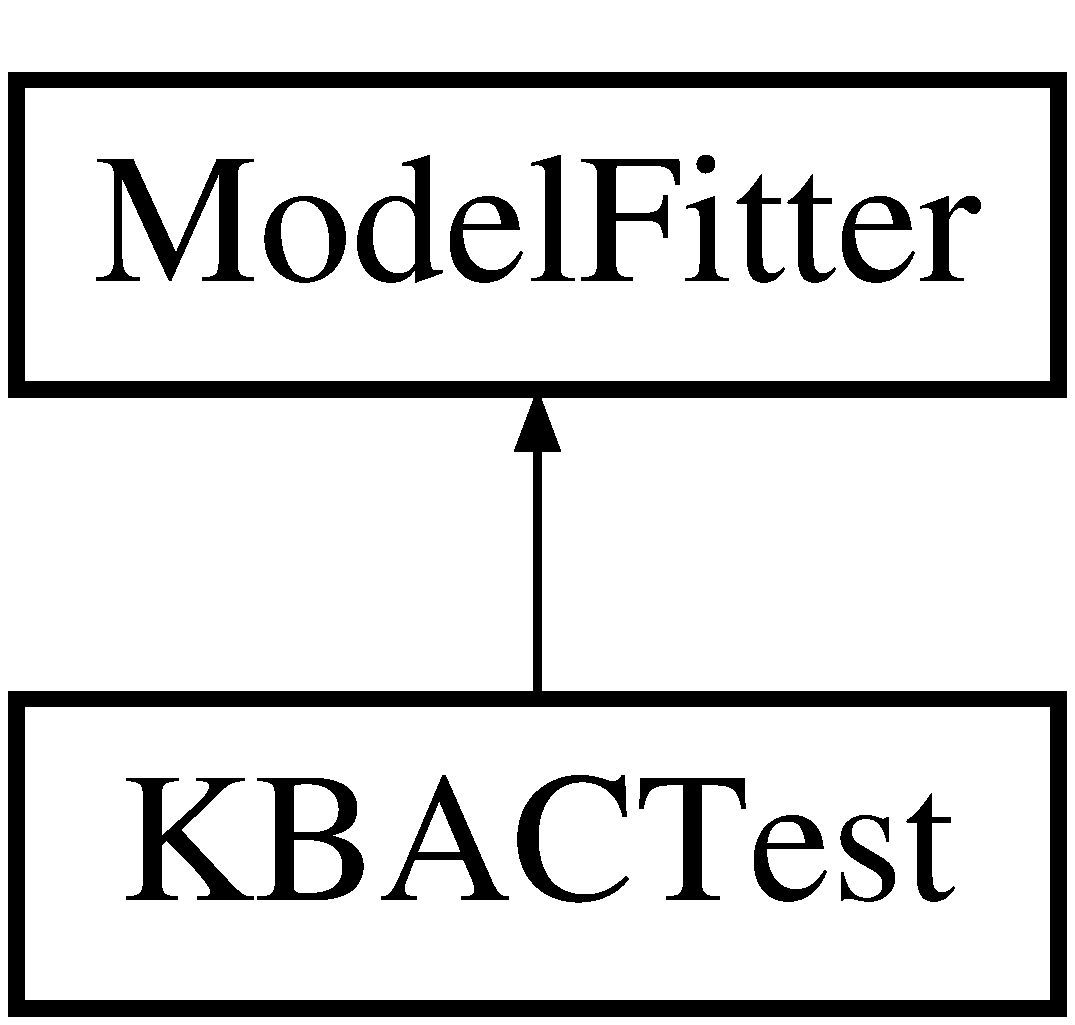
\includegraphics[height=2.000000cm]{classKBACTest}
\end{center}
\end{figure}
\subsection*{Public Member Functions}
\begin{DoxyCompactItemize}
\item 
\hypertarget{classKBACTest_a04db2b0a7c782d8c4a4e94f868fc2217}{{\bfseries K\-B\-A\-C\-Test} (int n\-Perm, double alpha)}\label{classKBACTest_a04db2b0a7c782d8c4a4e94f868fc2217}

\item 
\hypertarget{classKBACTest_a54a09e6a6bb1779ce7f1fcb49e7a2f2a}{void {\bfseries write\-Header} (File\-Writer $\ast$fp, const \hyperlink{classResult}{Result} \&site\-Info)}\label{classKBACTest_a54a09e6a6bb1779ce7f1fcb49e7a2f2a}

\item 
\hypertarget{classKBACTest_a975e1bf8ac13212efe9387e88bd19c63}{void {\bfseries reset} ()}\label{classKBACTest_a975e1bf8ac13212efe9387e88bd19c63}

\item 
int \hyperlink{classKBACTest_a4ebdf07477d26041b92ef5a63f4e1237}{fit} (\hyperlink{classDataConsolidator}{Data\-Consolidator} $\ast$dc)
\item 
\hypertarget{classKBACTest_a3836fbb6d6793ccb46a8e2037708b842}{void {\bfseries write\-Output} (File\-Writer $\ast$fp, const \hyperlink{classResult}{Result} \&site\-Info)}\label{classKBACTest_a3836fbb6d6793ccb46a8e2037708b842}

\item 
\hypertarget{classKBACTest_acf816107e17310c26f8e2720368292f5}{void {\bfseries resize} (int num\-People, int num\-Marker)}\label{classKBACTest_acf816107e17310c26f8e2720368292f5}

\end{DoxyCompactItemize}
\subsection*{Additional Inherited Members}


\subsection{Member Function Documentation}
\hypertarget{classKBACTest_a4ebdf07477d26041b92ef5a63f4e1237}{\index{K\-B\-A\-C\-Test@{K\-B\-A\-C\-Test}!fit@{fit}}
\index{fit@{fit}!KBACTest@{K\-B\-A\-C\-Test}}
\subsubsection[{fit}]{\setlength{\rightskip}{0pt plus 5cm}int K\-B\-A\-C\-Test\-::fit (
\begin{DoxyParamCaption}
\item[{{\bf Data\-Consolidator} $\ast$}]{dc}
\end{DoxyParamCaption}
)\hspace{0.3cm}{\ttfamily [inline]}, {\ttfamily [virtual]}}}\label{classKBACTest_a4ebdf07477d26041b92ef5a63f4e1237}
nn\-: number of permutation qq\-: quiet aa\-: alpha level maf\-Upper\-: M\-A\-F upper threshold xdat\-In\-: genotype matrix ydat\-In\-: phenotype matrix maf\-In\-: allele frequency for each marker of x xcol\-: number of column of genotype ylen\-: length of y

pvalue\-: results are here twosided\-: two sided tests or one sided test

Implements \hyperlink{classModelFitter}{Model\-Fitter}.



The documentation for this class was generated from the following file\-:\begin{DoxyCompactItemize}
\item 
Model\-Fitter.\-h\end{DoxyCompactItemize}

\hypertarget{classMadsonBrowningTest}{\section{Madson\-Browning\-Test Class Reference}
\label{classMadsonBrowningTest}\index{Madson\-Browning\-Test@{Madson\-Browning\-Test}}
}
Inheritance diagram for Madson\-Browning\-Test\-:\begin{figure}[H]
\begin{center}
\leavevmode
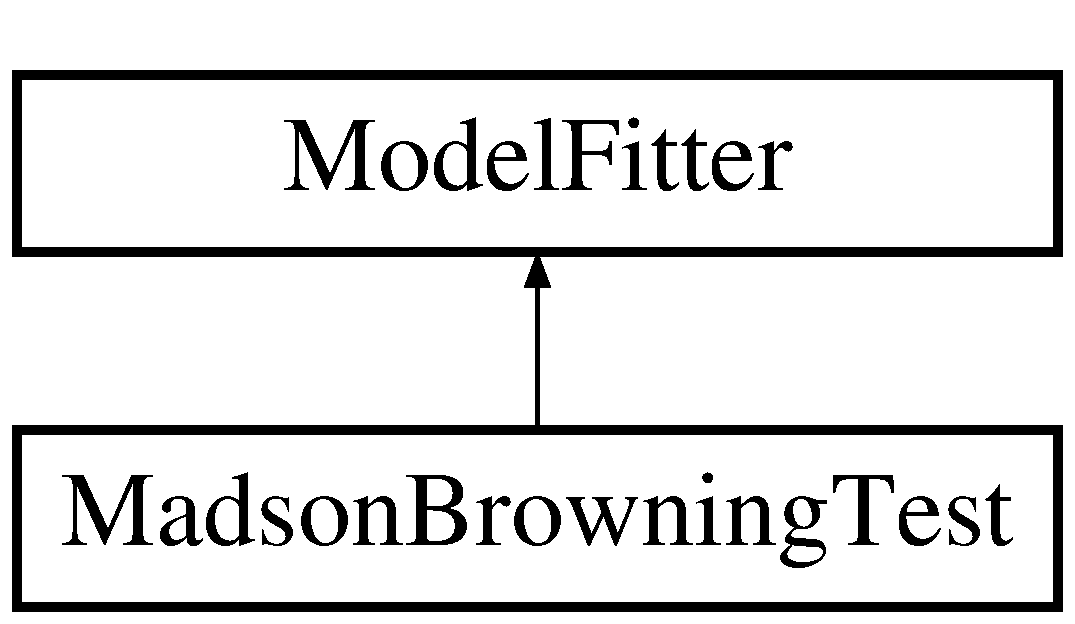
\includegraphics[height=2.000000cm]{classMadsonBrowningTest}
\end{center}
\end{figure}
\subsection*{Public Member Functions}
\begin{DoxyCompactItemize}
\item 
\hypertarget{classMadsonBrowningTest_a2f6a68960936fff6200a1b1eaf5791dd}{{\bfseries Madson\-Browning\-Test} (int n\-Perm, double alpha)}\label{classMadsonBrowningTest_a2f6a68960936fff6200a1b1eaf5791dd}

\item 
\hypertarget{classMadsonBrowningTest_a273b861db2af1cd83d8e1daf6084380b}{int {\bfseries fit} (\hyperlink{classDataConsolidator}{Data\-Consolidator} $\ast$dc)}\label{classMadsonBrowningTest_a273b861db2af1cd83d8e1daf6084380b}

\item 
\hypertarget{classMadsonBrowningTest_aab14718f5c6936b1e9887e871c914644}{void {\bfseries reset} ()}\label{classMadsonBrowningTest_aab14718f5c6936b1e9887e871c914644}

\item 
\hypertarget{classMadsonBrowningTest_a146e7e7454d9637c2102228da68903fa}{void {\bfseries write\-Header} (File\-Writer $\ast$fp, const \hyperlink{classResult}{Result} \&site\-Info)}\label{classMadsonBrowningTest_a146e7e7454d9637c2102228da68903fa}

\item 
\hypertarget{classMadsonBrowningTest_ac4d19c457d198fd30178c71af5a801f0}{void {\bfseries write\-Output} (File\-Writer $\ast$fp, const \hyperlink{classResult}{Result} \&site\-Info)}\label{classMadsonBrowningTest_ac4d19c457d198fd30178c71af5a801f0}

\end{DoxyCompactItemize}
\subsection*{Additional Inherited Members}


The documentation for this class was generated from the following file\-:\begin{DoxyCompactItemize}
\item 
Model\-Fitter.\-h\end{DoxyCompactItemize}

\hypertarget{classMetaCovTest}{\section{Meta\-Cov\-Test Class Reference}
\label{classMetaCovTest}\index{Meta\-Cov\-Test@{Meta\-Cov\-Test}}
}
Inheritance diagram for Meta\-Cov\-Test\-:\begin{figure}[H]
\begin{center}
\leavevmode
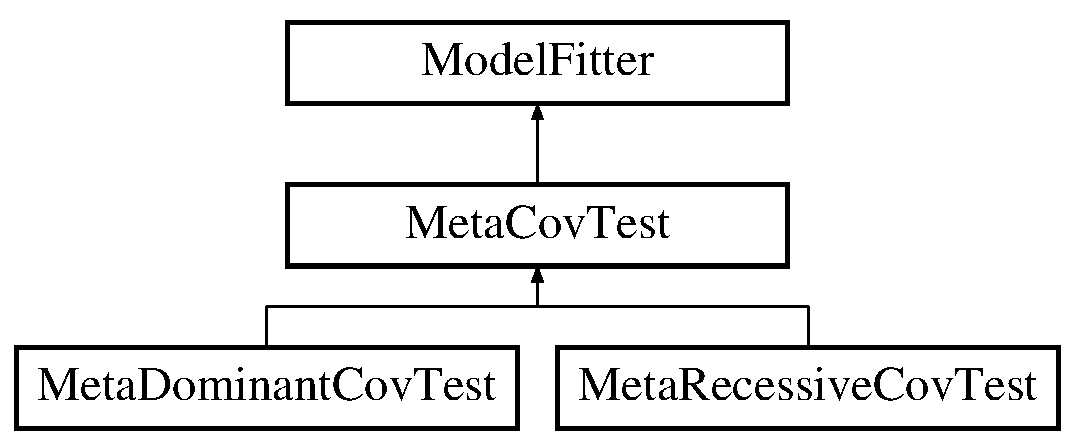
\includegraphics[height=3.000000cm]{classMetaCovTest}
\end{center}
\end{figure}
\subsection*{Classes}
\begin{DoxyCompactItemize}
\item 
struct {\bfseries Loci}
\item 
struct {\bfseries Pos}
\end{DoxyCompactItemize}
\subsection*{Public Member Functions}
\begin{DoxyCompactItemize}
\item 
\hypertarget{classMetaCovTest_a589b87655c0d10c98c4136268943794d}{{\bfseries Meta\-Cov\-Test} (int window\-Size)}\label{classMetaCovTest_a589b87655c0d10c98c4136268943794d}

\item 
\hypertarget{classMetaCovTest_a5a90d2fffcc1b8fde287fab7621aa91a}{virtual int {\bfseries fit} (\hyperlink{classDataConsolidator}{Data\-Consolidator} $\ast$dc)}\label{classMetaCovTest_a5a90d2fffcc1b8fde287fab7621aa91a}

\item 
int \hyperlink{classMetaCovTest_a23270f699cbcd9a3d4e6091da9cdd229}{fit\-With\-Given\-Genotype} (Matrix \&genotype, \hyperlink{classDataConsolidator}{Data\-Consolidator} $\ast$dc)
\item 
\hypertarget{classMetaCovTest_a05039515e319256c1f330bf7dc3d72af}{void {\bfseries write\-Header} (File\-Writer $\ast$fp, const \hyperlink{classResult}{Result} \&site\-Info)}\label{classMetaCovTest_a05039515e319256c1f330bf7dc3d72af}

\item 
\hypertarget{classMetaCovTest_aa6557da8838f8e59005796beda41be58}{void {\bfseries write\-Output} (File\-Writer $\ast$fp, const \hyperlink{classResult}{Result} \&site\-Info)}\label{classMetaCovTest_aa6557da8838f8e59005796beda41be58}

\end{DoxyCompactItemize}
\subsection*{Additional Inherited Members}


\subsection{Member Function Documentation}
\hypertarget{classMetaCovTest_a23270f699cbcd9a3d4e6091da9cdd229}{\index{Meta\-Cov\-Test@{Meta\-Cov\-Test}!fit\-With\-Given\-Genotype@{fit\-With\-Given\-Genotype}}
\index{fit\-With\-Given\-Genotype@{fit\-With\-Given\-Genotype}!MetaCovTest@{Meta\-Cov\-Test}}
\subsubsection[{fit\-With\-Given\-Genotype}]{\setlength{\rightskip}{0pt plus 5cm}int Meta\-Cov\-Test\-::fit\-With\-Given\-Genotype (
\begin{DoxyParamCaption}
\item[{Matrix \&}]{genotype, }
\item[{{\bf Data\-Consolidator} $\ast$}]{dc}
\end{DoxyParamCaption}
)\hspace{0.3cm}{\ttfamily [inline]}}}\label{classMetaCovTest_a23270f699cbcd9a3d4e6091da9cdd229}
for binary, no need to center. and not support family. 

The documentation for this class was generated from the following file\-:\begin{DoxyCompactItemize}
\item 
Model\-Fitter.\-h\end{DoxyCompactItemize}

\hypertarget{classMetaDominantCovTest}{\section{Meta\-Dominant\-Cov\-Test Class Reference}
\label{classMetaDominantCovTest}\index{Meta\-Dominant\-Cov\-Test@{Meta\-Dominant\-Cov\-Test}}
}
Inheritance diagram for Meta\-Dominant\-Cov\-Test\-:\begin{figure}[H]
\begin{center}
\leavevmode
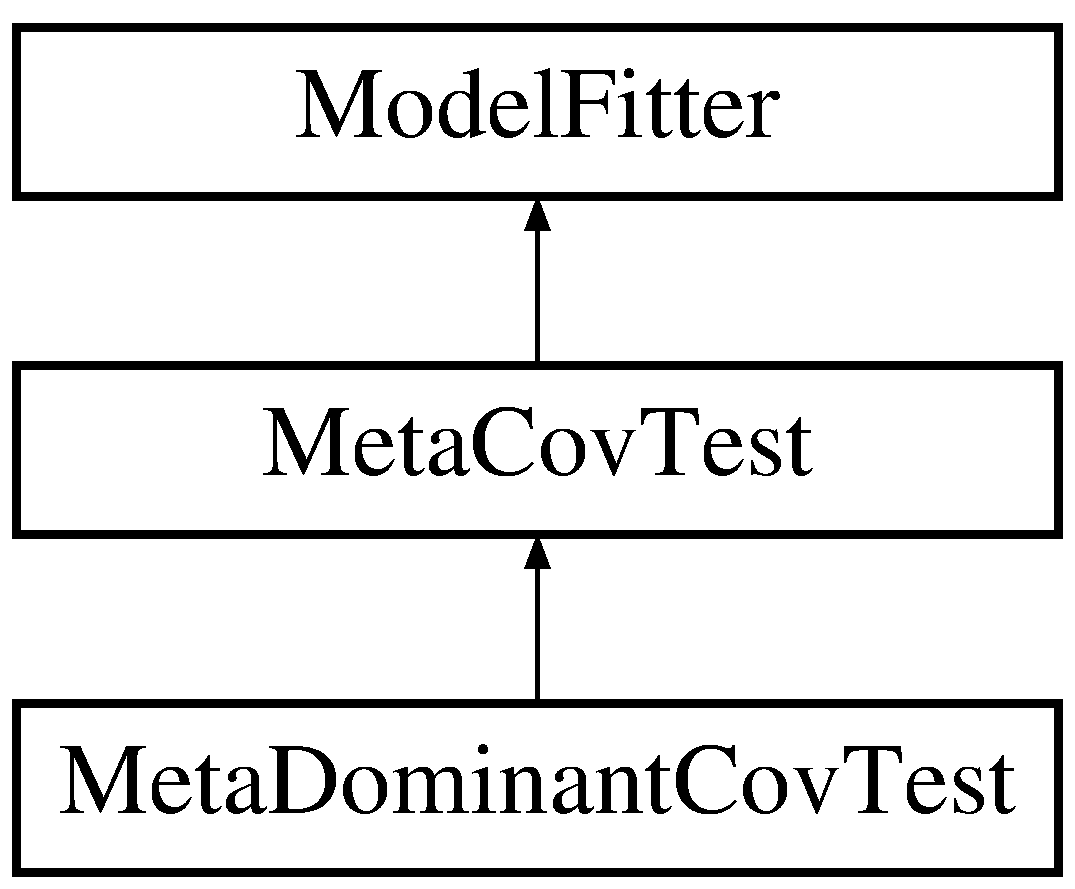
\includegraphics[height=3.000000cm]{classMetaDominantCovTest}
\end{center}
\end{figure}
\subsection*{Public Member Functions}
\begin{DoxyCompactItemize}
\item 
\hypertarget{classMetaDominantCovTest_a1aa23cc690a8c8d4afac3eedf96feab7}{{\bfseries Meta\-Dominant\-Cov\-Test} (int window\-Size)}\label{classMetaDominantCovTest_a1aa23cc690a8c8d4afac3eedf96feab7}

\item 
\hypertarget{classMetaDominantCovTest_aaf8b4091a56092f5721f4cdc5f62332f}{virtual int {\bfseries fit} (\hyperlink{classDataConsolidator}{Data\-Consolidator} $\ast$dc)}\label{classMetaDominantCovTest_aaf8b4091a56092f5721f4cdc5f62332f}

\end{DoxyCompactItemize}
\subsection*{Additional Inherited Members}


The documentation for this class was generated from the following file\-:\begin{DoxyCompactItemize}
\item 
Model\-Fitter.\-h\end{DoxyCompactItemize}

\hypertarget{classMetaDominantTest}{\section{Meta\-Dominant\-Test Class Reference}
\label{classMetaDominantTest}\index{Meta\-Dominant\-Test@{Meta\-Dominant\-Test}}
}
Inheritance diagram for Meta\-Dominant\-Test\-:\begin{figure}[H]
\begin{center}
\leavevmode
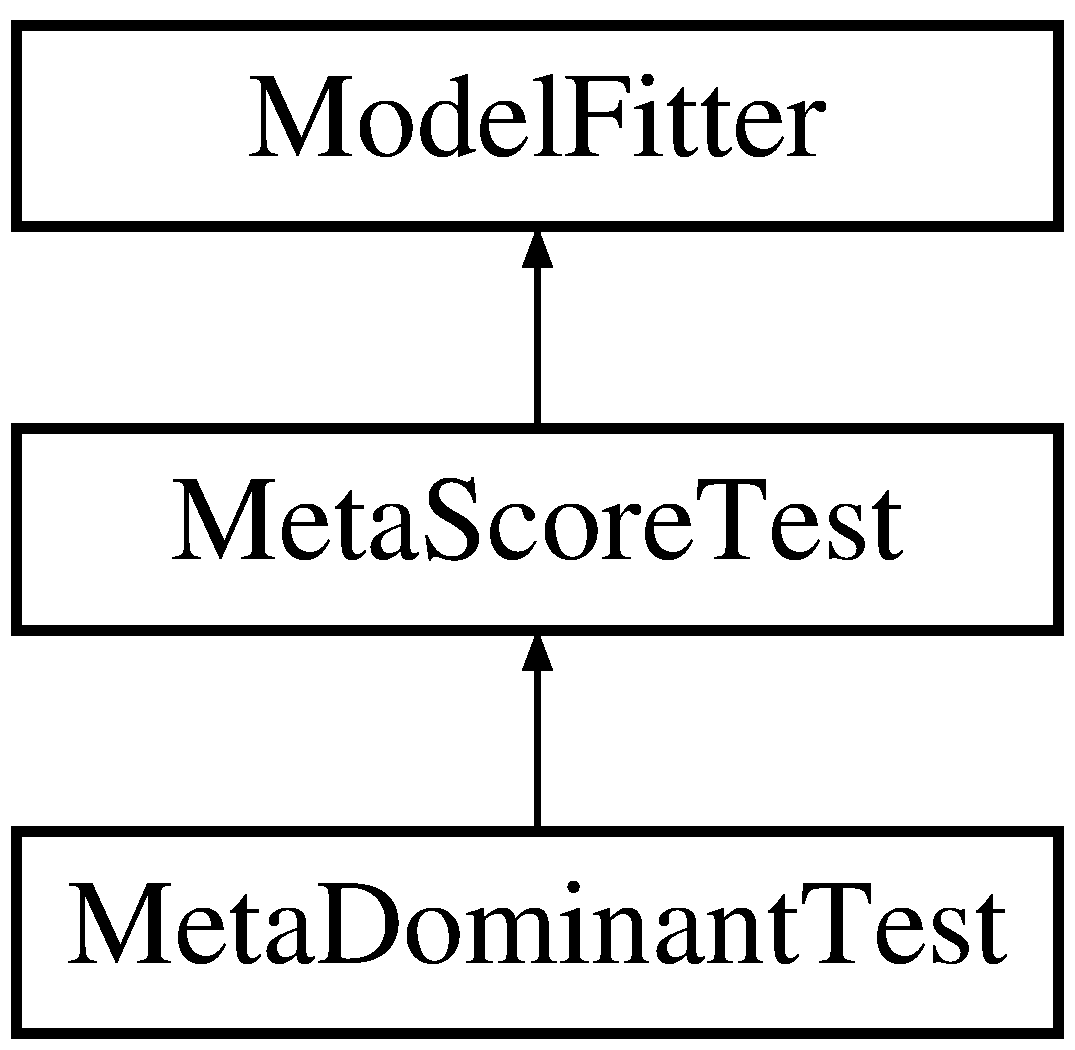
\includegraphics[height=3.000000cm]{classMetaDominantTest}
\end{center}
\end{figure}
\subsection*{Public Member Functions}
\begin{DoxyCompactItemize}
\item 
\hypertarget{classMetaDominantTest_a12c7e00e7734172c746ddce233bb3835}{virtual int {\bfseries fit} (\hyperlink{classDataConsolidator}{Data\-Consolidator} $\ast$dc)}\label{classMetaDominantTest_a12c7e00e7734172c746ddce233bb3835}

\end{DoxyCompactItemize}
\subsection*{Additional Inherited Members}


The documentation for this class was generated from the following file\-:\begin{DoxyCompactItemize}
\item 
Model\-Fitter.\-h\end{DoxyCompactItemize}

\hypertarget{classMetaRecessiveCovTest}{\section{Meta\-Recessive\-Cov\-Test Class Reference}
\label{classMetaRecessiveCovTest}\index{Meta\-Recessive\-Cov\-Test@{Meta\-Recessive\-Cov\-Test}}
}
Inheritance diagram for Meta\-Recessive\-Cov\-Test\-:\begin{figure}[H]
\begin{center}
\leavevmode
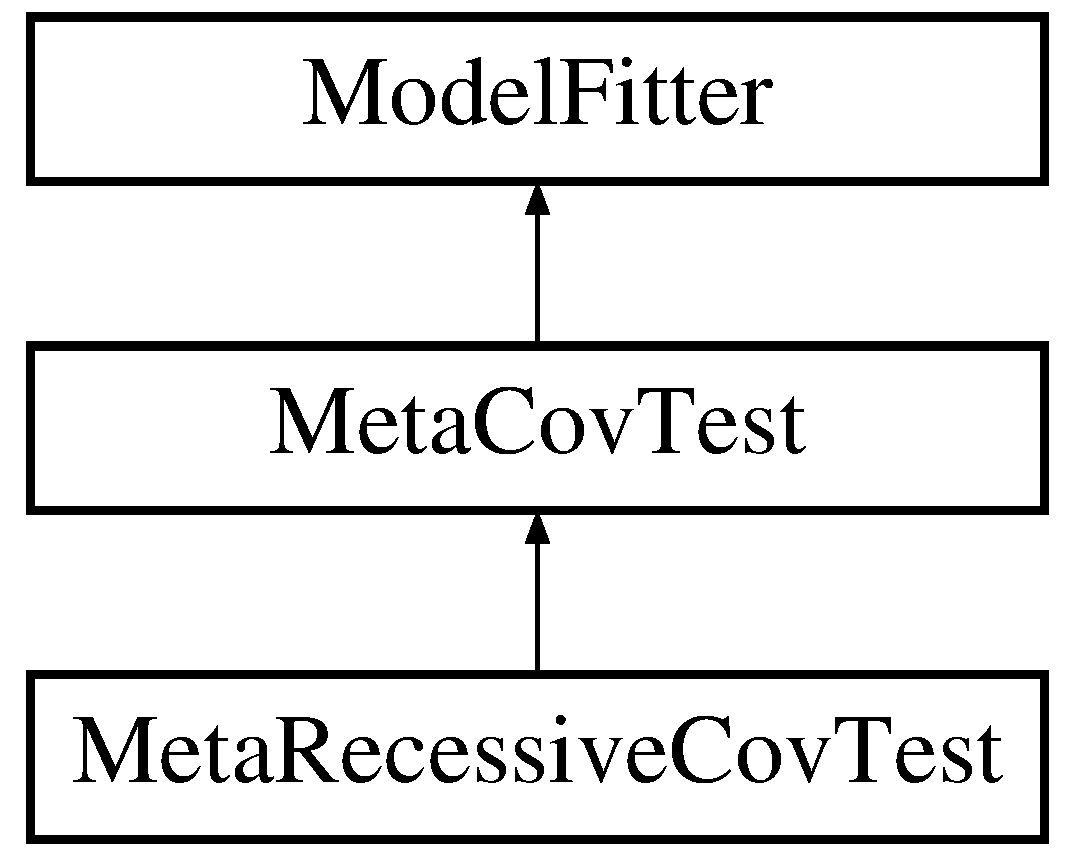
\includegraphics[height=3.000000cm]{classMetaRecessiveCovTest}
\end{center}
\end{figure}
\subsection*{Public Member Functions}
\begin{DoxyCompactItemize}
\item 
\hypertarget{classMetaRecessiveCovTest_aa10e966ebff6541531e03def7f8706aa}{{\bfseries Meta\-Recessive\-Cov\-Test} (int window\-Size)}\label{classMetaRecessiveCovTest_aa10e966ebff6541531e03def7f8706aa}

\item 
\hypertarget{classMetaRecessiveCovTest_a7378e98f9f7305ea75778c0f4d7c618d}{virtual int {\bfseries fit} (\hyperlink{classDataConsolidator}{Data\-Consolidator} $\ast$dc)}\label{classMetaRecessiveCovTest_a7378e98f9f7305ea75778c0f4d7c618d}

\end{DoxyCompactItemize}
\subsection*{Additional Inherited Members}


The documentation for this class was generated from the following file\-:\begin{DoxyCompactItemize}
\item 
Model\-Fitter.\-h\end{DoxyCompactItemize}

\hypertarget{classMetaRecessiveTest}{\section{Meta\-Recessive\-Test Class Reference}
\label{classMetaRecessiveTest}\index{Meta\-Recessive\-Test@{Meta\-Recessive\-Test}}
}
Inheritance diagram for Meta\-Recessive\-Test\-:\begin{figure}[H]
\begin{center}
\leavevmode
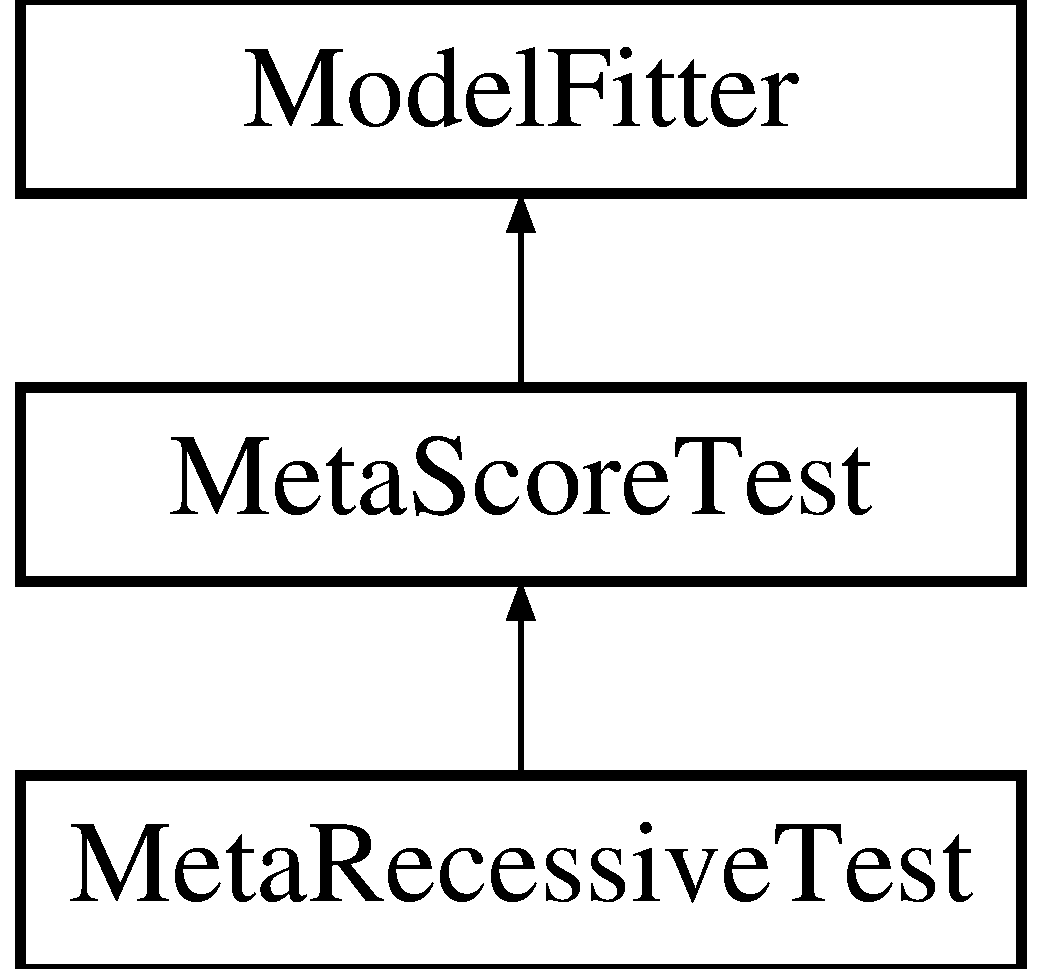
\includegraphics[height=3.000000cm]{classMetaRecessiveTest}
\end{center}
\end{figure}
\subsection*{Public Member Functions}
\begin{DoxyCompactItemize}
\item 
\hypertarget{classMetaRecessiveTest_a6327391bd4f2e2a0a3bf6367a6cbde78}{virtual int {\bfseries fit} (\hyperlink{classDataConsolidator}{Data\-Consolidator} $\ast$dc)}\label{classMetaRecessiveTest_a6327391bd4f2e2a0a3bf6367a6cbde78}

\end{DoxyCompactItemize}
\subsection*{Additional Inherited Members}


The documentation for this class was generated from the following file\-:\begin{DoxyCompactItemize}
\item 
Model\-Fitter.\-h\end{DoxyCompactItemize}

\hypertarget{classMetaScoreTest}{\section{Meta\-Score\-Test Class Reference}
\label{classMetaScoreTest}\index{Meta\-Score\-Test@{Meta\-Score\-Test}}
}
Inheritance diagram for Meta\-Score\-Test\-:\begin{figure}[H]
\begin{center}
\leavevmode
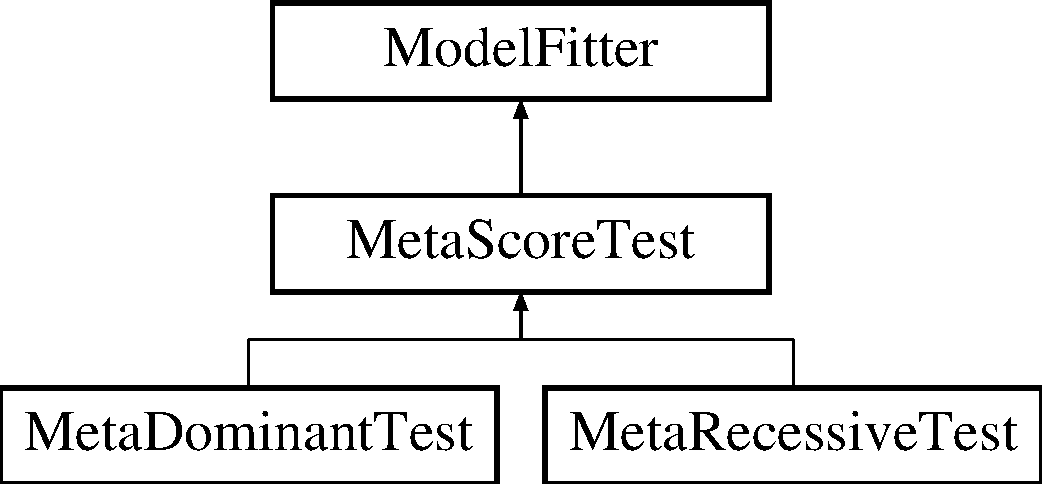
\includegraphics[height=3.000000cm]{classMetaScoreTest}
\end{center}
\end{figure}
\subsection*{Public Member Functions}
\begin{DoxyCompactItemize}
\item 
\hypertarget{classMetaScoreTest_a3342caf82dc635e98b676e6e43254fee}{virtual int {\bfseries fit} (\hyperlink{classDataConsolidator}{Data\-Consolidator} $\ast$dc)}\label{classMetaScoreTest_a3342caf82dc635e98b676e6e43254fee}

\item 
\hypertarget{classMetaScoreTest_a48b8ec26ac543a624308211daf486d1a}{int {\bfseries fit\-With\-Given\-Genotype} (Matrix \&genotype, \hyperlink{classDataConsolidator}{Data\-Consolidator} $\ast$dc)}\label{classMetaScoreTest_a48b8ec26ac543a624308211daf486d1a}

\item 
\hypertarget{classMetaScoreTest_ab6611f67774d393a0f8dc1af3c9ea702}{void {\bfseries write\-Header} (File\-Writer $\ast$fp, const \hyperlink{classResult}{Result} \&site\-Info)}\label{classMetaScoreTest_ab6611f67774d393a0f8dc1af3c9ea702}

\item 
\hypertarget{classMetaScoreTest_a31b12746201ee0ab0934e378a5e9abc9}{void {\bfseries write\-Output} (File\-Writer $\ast$fp, const \hyperlink{classResult}{Result} \&site\-Info)}\label{classMetaScoreTest_a31b12746201ee0ab0934e378a5e9abc9}

\item 
\hypertarget{classMetaScoreTest_ad69f7aba1bdb77dec7148c8568477131}{void {\bfseries write\-Footnote} (File\-Writer $\ast$fp)}\label{classMetaScoreTest_ad69f7aba1bdb77dec7148c8568477131}

\end{DoxyCompactItemize}
\subsection*{Additional Inherited Members}


The documentation for this class was generated from the following file\-:\begin{DoxyCompactItemize}
\item 
Model\-Fitter.\-h\end{DoxyCompactItemize}

\hypertarget{classModelFitter}{\section{Model\-Fitter Class Reference}
\label{classModelFitter}\index{Model\-Fitter@{Model\-Fitter}}
}
Inheritance diagram for Model\-Fitter\-:\begin{figure}[H]
\begin{center}
\leavevmode
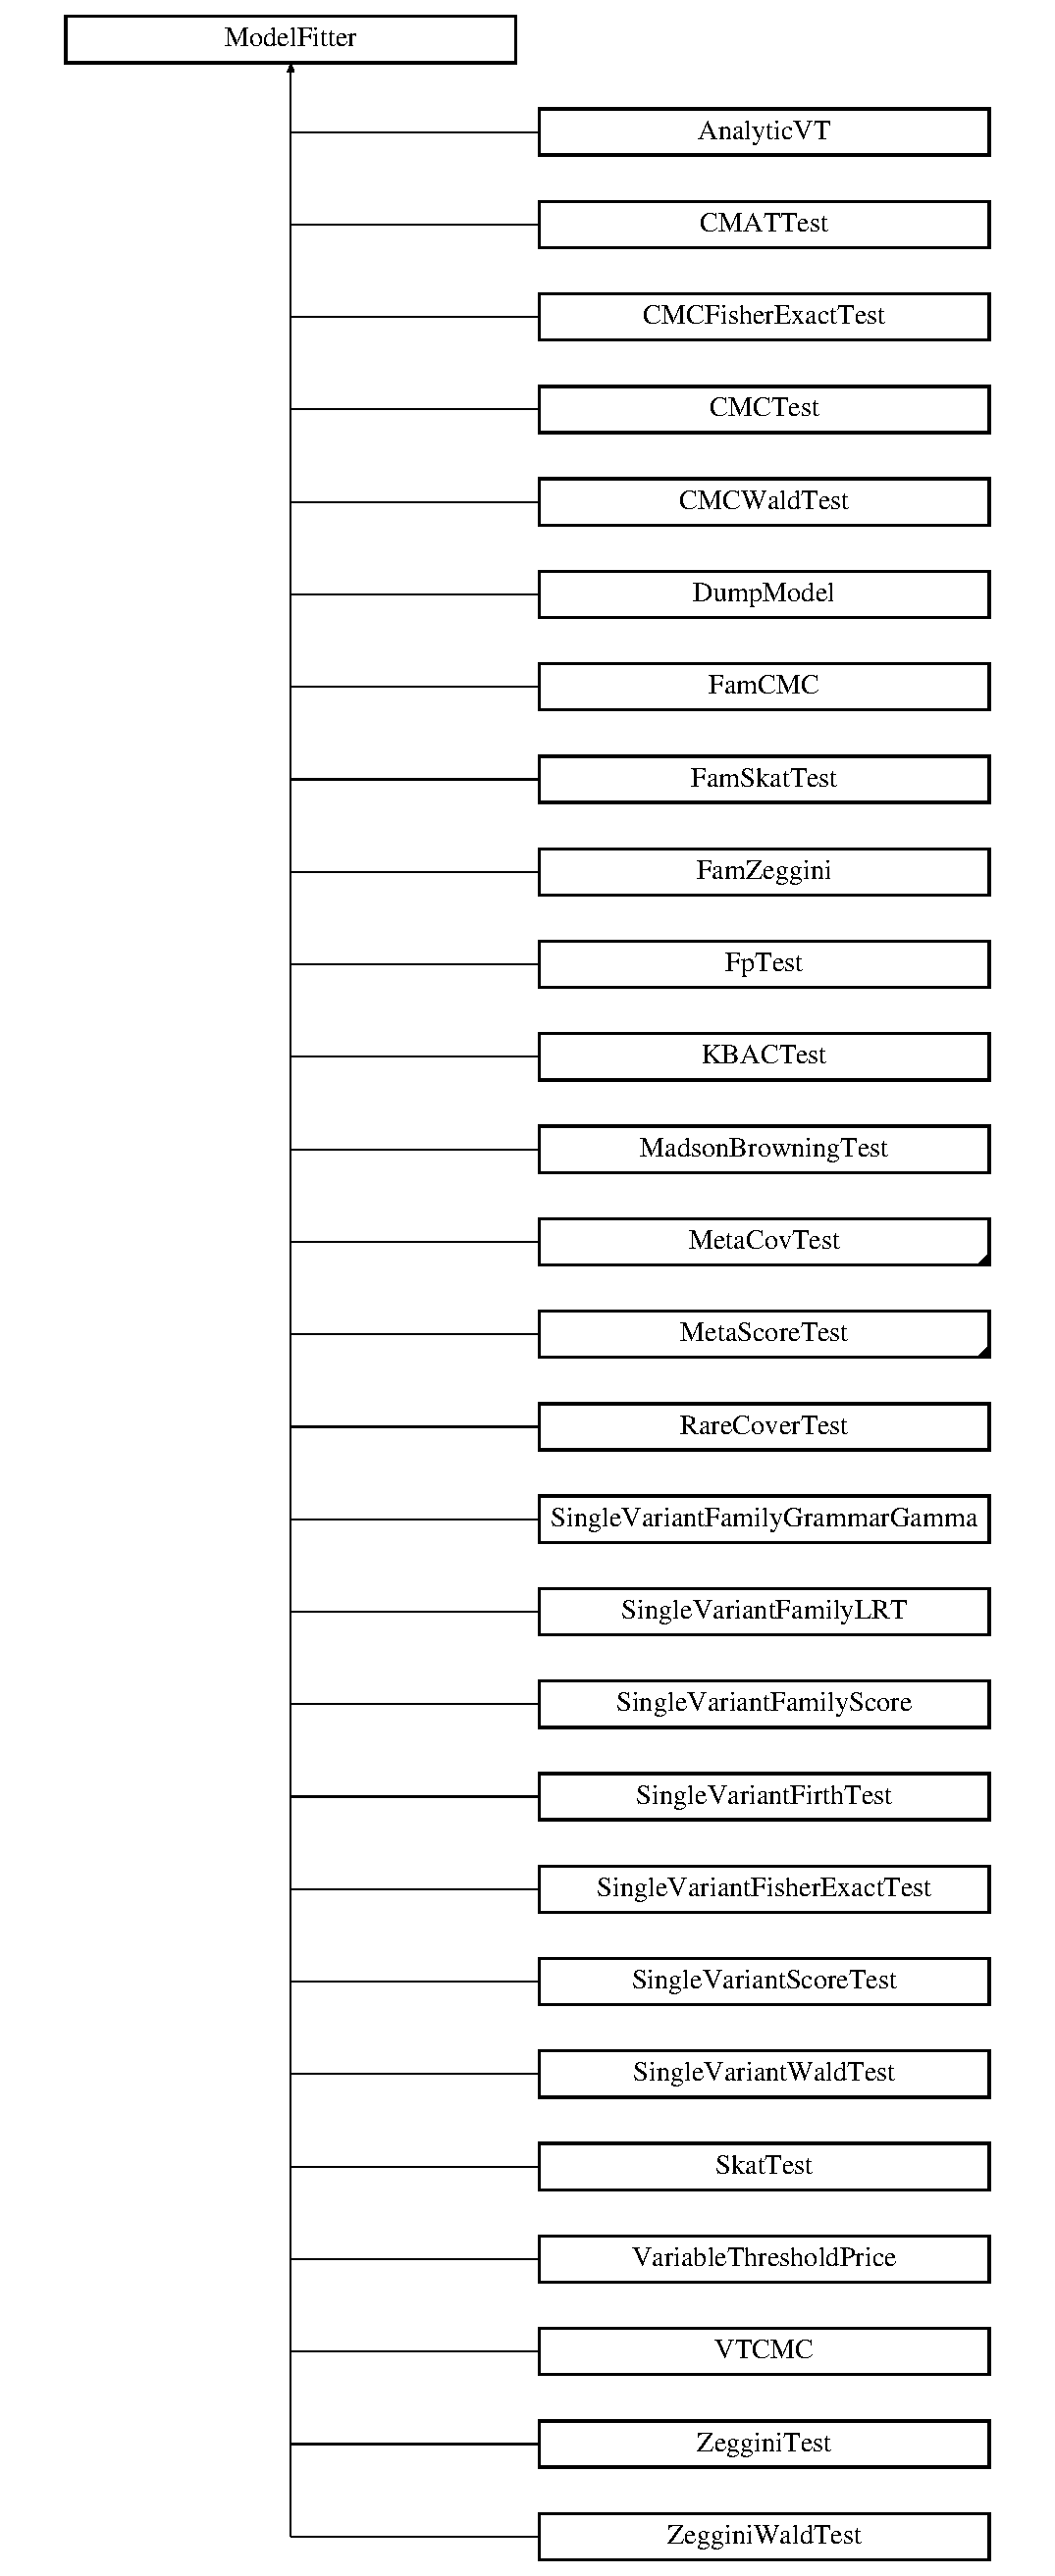
\includegraphics[height=12.000000cm]{classModelFitter}
\end{center}
\end{figure}
\subsection*{Public Member Functions}
\begin{DoxyCompactItemize}
\item 
\hypertarget{classModelFitter_afc83ca5c7ac8a67c8a9d29ec3c57b5e7}{virtual int {\bfseries fit} (\hyperlink{classDataConsolidator}{Data\-Consolidator} $\ast$dc)=0}\label{classModelFitter_afc83ca5c7ac8a67c8a9d29ec3c57b5e7}

\item 
\hypertarget{classModelFitter_a278e57cc5d181a7b35c107322ae527a0}{virtual void {\bfseries write\-Header} (File\-Writer $\ast$fp, const \hyperlink{classResult}{Result} \&site\-Info)=0}\label{classModelFitter_a278e57cc5d181a7b35c107322ae527a0}

\item 
\hypertarget{classModelFitter_a3943a0d27e67b6223c0ae35de19bcf16}{virtual void {\bfseries write\-Output} (File\-Writer $\ast$fp, const \hyperlink{classResult}{Result} \&site\-Info)=0}\label{classModelFitter_a3943a0d27e67b6223c0ae35de19bcf16}

\item 
\hypertarget{classModelFitter_ad71117c9dec501a879e35c47dbd06096}{virtual void {\bfseries write\-Footnote} (File\-Writer $\ast$fp)}\label{classModelFitter_ad71117c9dec501a879e35c47dbd06096}

\item 
\hypertarget{classModelFitter_ade717703169cd941319520567f4d0e71}{const std\-::string \& {\bfseries get\-Model\-Name} () const }\label{classModelFitter_ade717703169cd941319520567f4d0e71}

\item 
\hypertarget{classModelFitter_a533cc2f91ad6a55a1dab1f4f28833da9}{virtual void {\bfseries reset} ()}\label{classModelFitter_a533cc2f91ad6a55a1dab1f4f28833da9}

\item 
\hypertarget{classModelFitter_a1f1037669ff3a4b564e7787516bc75fc}{bool {\bfseries is\-Binary\-Outcome} () const }\label{classModelFitter_a1f1037669ff3a4b564e7787516bc75fc}

\item 
\hypertarget{classModelFitter_ad81b3fa897788405095cd405604b223a}{void {\bfseries set\-Binary\-Outcome} ()}\label{classModelFitter_ad81b3fa897788405095cd405604b223a}

\item 
\hypertarget{classModelFitter_a93c9f18c48b73e6f4cdd66b4d0a83e5c}{void {\bfseries set\-Continuous\-Outcome} ()}\label{classModelFitter_a93c9f18c48b73e6f4cdd66b4d0a83e5c}

\item 
\hypertarget{classModelFitter_a357f8d42cd176127a8ebf578e28e4c22}{const \hyperlink{classResult}{Result} \& {\bfseries get\-Result} () const }\label{classModelFitter_a357f8d42cd176127a8ebf578e28e4c22}

\end{DoxyCompactItemize}
\subsection*{Protected Attributes}
\begin{DoxyCompactItemize}
\item 
\hypertarget{classModelFitter_acf837c9a65e7c0626a3f0f1b4d3c2dac}{std\-::string {\bfseries model\-Name}}\label{classModelFitter_acf837c9a65e7c0626a3f0f1b4d3c2dac}

\item 
\hypertarget{classModelFitter_a82e7d062d0e12c7fdf31263361c39e47}{bool {\bfseries binary\-Outcome}}\label{classModelFitter_a82e7d062d0e12c7fdf31263361c39e47}

\item 
\hypertarget{classModelFitter_a0189c3de8ff8cf73d885fc2af170a754}{\hyperlink{classResult}{Result} {\bfseries result}}\label{classModelFitter_a0189c3de8ff8cf73d885fc2af170a754}

\end{DoxyCompactItemize}


The documentation for this class was generated from the following file\-:\begin{DoxyCompactItemize}
\item 
Model\-Fitter.\-h\end{DoxyCompactItemize}

\hypertarget{classModelParser}{\section{Model\-Parser Class Reference}
\label{classModelParser}\index{Model\-Parser@{Model\-Parser}}
}


{\ttfamily \#include $<$Model\-Parser.\-h$>$}

\subsection*{Public Member Functions}
\begin{DoxyCompactItemize}
\item 
int \hyperlink{classModelParser_a83a5484f3fa5e80242216cb0d08180a4}{parse} (const std\-::string \&s)
\item 
\hypertarget{classModelParser_aab017724228e05e104c48b65e6591965}{const std\-::string \& {\bfseries get\-Name} () const }\label{classModelParser_aab017724228e05e104c48b65e6591965}

\item 
\hypertarget{classModelParser_a48674af5a50b124b86194864385af517}{bool {\bfseries has\-Tag} (const std\-::string \&tag) const }\label{classModelParser_a48674af5a50b124b86194864385af517}

\item 
\hypertarget{classModelParser_aaed7ae55cc66c1c4fcd38672be12d712}{const char $\ast$ {\bfseries value} (const std\-::string \&tag) const }\label{classModelParser_aaed7ae55cc66c1c4fcd38672be12d712}

\item 
\hyperlink{classModelParser}{Model\-Parser} \& \hyperlink{classModelParser_a29363d37f73bcc655c995d30d662cc08}{assign} (const std\-::string \&tag, bool $\ast$value)
\item 
\hypertarget{classModelParser_af62115ed375db3e8909932f3636d09d4}{\hyperlink{classModelParser}{Model\-Parser} \& {\bfseries assign} (const std\-::string \&tag, double $\ast$value)}\label{classModelParser_af62115ed375db3e8909932f3636d09d4}

\item 
\hypertarget{classModelParser_abd272e8dc6db873c3b6d3e2f85179124}{\hyperlink{classModelParser}{Model\-Parser} \& {\bfseries assign} (const std\-::string \&tag, int $\ast$value)}\label{classModelParser_abd272e8dc6db873c3b6d3e2f85179124}

\item 
\hypertarget{classModelParser_a26bb6bf4aee749a358ffe77ea616bd60}{\hyperlink{classModelParser}{Model\-Parser} \& {\bfseries assign} (const std\-::string \&tag, std\-::string $\ast$value)}\label{classModelParser_a26bb6bf4aee749a358ffe77ea616bd60}

\item 
\hyperlink{classModelParser}{Model\-Parser} \& \hyperlink{classModelParser_ac3c7dc0f7484ebd31cf54cc8b9a0c577}{assign} (const std\-::string \&tag, bool $\ast$value, const bool def)
\item 
\hypertarget{classModelParser_a03a38e94224700ff73332930d9d43e4a}{\hyperlink{classModelParser}{Model\-Parser} \& {\bfseries assign} (const std\-::string \&tag, double $\ast$value, const double def)}\label{classModelParser_a03a38e94224700ff73332930d9d43e4a}

\item 
\hypertarget{classModelParser_aeed128d82ced7586870cd293fee36264}{\hyperlink{classModelParser}{Model\-Parser} \& {\bfseries assign} (const std\-::string \&tag, int $\ast$value, const int def)}\label{classModelParser_aeed128d82ced7586870cd293fee36264}

\item 
\hypertarget{classModelParser_aefce479b7f56bfbe74d79110edf01e49}{\hyperlink{classModelParser}{Model\-Parser} \& {\bfseries assign} (const std\-::string \&tag, std\-::string $\ast$value, const std\-::string \&def)}\label{classModelParser_aefce479b7f56bfbe74d79110edf01e49}

\item 
\hypertarget{classModelParser_a7c0cdad1d8b8a7c0aee6c0ae07664363}{const size\-\_\-t {\bfseries size} () const }\label{classModelParser_a7c0cdad1d8b8a7c0aee6c0ae07664363}

\end{DoxyCompactItemize}
\subsection*{Static Public Attributes}
\begin{DoxyCompactItemize}
\item 
\hypertarget{classModelParser_aac2c439ee878395e385046a1f5aafc48}{static const char {\bfseries L\-E\-F\-T\-\_\-\-D\-E\-L\-I\-M} = '\mbox{[}'}\label{classModelParser_aac2c439ee878395e385046a1f5aafc48}

\item 
\hypertarget{classModelParser_a185a34c33b9648946627a5b06ae1a741}{static const char {\bfseries R\-I\-G\-H\-T\-\_\-\-D\-E\-L\-I\-M} = '\mbox{]}'}\label{classModelParser_a185a34c33b9648946627a5b06ae1a741}

\item 
\hypertarget{classModelParser_a1811dec15667074357233d6df7f44939}{static const char {\bfseries P\-A\-R\-A\-M\-\_\-\-D\-E\-L\-I\-M} = '\-:'}\label{classModelParser_a1811dec15667074357233d6df7f44939}

\end{DoxyCompactItemize}


\subsection{Detailed Description}
Parse \char`\"{}mb\char`\"{} to \{\char`\"{}mb\char`\"{}\} Parse \char`\"{}mb(nperm=10000, alpha=0.\-1)\char`\"{} then later use assign(\char`\"{}nperm\char`\"{}, \&p) to set value for p 

\subsection{Member Function Documentation}
\hypertarget{classModelParser_a29363d37f73bcc655c995d30d662cc08}{\index{Model\-Parser@{Model\-Parser}!assign@{assign}}
\index{assign@{assign}!ModelParser@{Model\-Parser}}
\subsubsection[{assign}]{\setlength{\rightskip}{0pt plus 5cm}{\bf Model\-Parser}\& Model\-Parser\-::assign (
\begin{DoxyParamCaption}
\item[{const std\-::string \&}]{tag, }
\item[{bool $\ast$}]{value}
\end{DoxyParamCaption}
)\hspace{0.3cm}{\ttfamily [inline]}}}\label{classModelParser_a29363d37f73bcc655c995d30d662cc08}
assign 
\begin{DoxyParams}{Parameters}
{\em tag} & to \\
\hline
{\em value} & \\
\hline
\end{DoxyParams}
\hypertarget{classModelParser_ac3c7dc0f7484ebd31cf54cc8b9a0c577}{\index{Model\-Parser@{Model\-Parser}!assign@{assign}}
\index{assign@{assign}!ModelParser@{Model\-Parser}}
\subsubsection[{assign}]{\setlength{\rightskip}{0pt plus 5cm}{\bf Model\-Parser}\& Model\-Parser\-::assign (
\begin{DoxyParamCaption}
\item[{const std\-::string \&}]{tag, }
\item[{bool $\ast$}]{value, }
\item[{const bool}]{def}
\end{DoxyParamCaption}
)\hspace{0.3cm}{\ttfamily [inline]}}}\label{classModelParser_ac3c7dc0f7484ebd31cf54cc8b9a0c577}
if 
\begin{DoxyParams}{Parameters}
{\em tag} & is provided, assign \\
\hline
{\em tag} & to \\
\hline
{\em value} & otherwise, set \\
\hline
{\em value} & to \\
\hline
{\em def} & \\
\hline
\end{DoxyParams}
\hypertarget{classModelParser_a83a5484f3fa5e80242216cb0d08180a4}{\index{Model\-Parser@{Model\-Parser}!parse@{parse}}
\index{parse@{parse}!ModelParser@{Model\-Parser}}
\subsubsection[{parse}]{\setlength{\rightskip}{0pt plus 5cm}int Model\-Parser\-::parse (
\begin{DoxyParamCaption}
\item[{const std\-::string \&}]{s}
\end{DoxyParamCaption}
)\hspace{0.3cm}{\ttfamily [inline]}}}\label{classModelParser_a83a5484f3fa5e80242216cb0d08180a4}
\begin{DoxyReturn}{Returns}
0\-: if parse succeed. N\-O\-T\-E\-: will convert all letters to lower case 
\end{DoxyReturn}


The documentation for this class was generated from the following file\-:\begin{DoxyCompactItemize}
\item 
Model\-Parser.\-h\end{DoxyCompactItemize}

\hypertarget{classPermutation}{\section{Permutation Class Reference}
\label{classPermutation}\index{Permutation@{Permutation}}
}
\subsection*{Public Member Functions}
\begin{DoxyCompactItemize}
\item 
\hypertarget{classPermutation_a265c2e656ff622e587108bf78fd6eaee}{{\bfseries Permutation} (int n\-Perm, double alpha)}\label{classPermutation_a265c2e656ff622e587108bf78fd6eaee}

\item 
void \hyperlink{classPermutation_a6253565860ce50c687a01ab6bfe4af2d}{init} (double observation)
\item 
bool \hyperlink{classPermutation_afe33da36f035988a7edf0d131119d26c}{next} ()
\item 
\hypertarget{classPermutation_aead055d6fa313f827a852d53018cf8b2}{void {\bfseries add} (double s)}\label{classPermutation_aead055d6fa313f827a852d53018cf8b2}

\item 
\hypertarget{classPermutation_aa9559076625fb951293dab295d426e32}{double {\bfseries get\-Pvalue} () const }\label{classPermutation_aa9559076625fb951293dab295d426e32}

\item 
\hypertarget{classPermutation_a03558b5588a16e736ce47210dd2d7160}{void {\bfseries reset} ()}\label{classPermutation_a03558b5588a16e736ce47210dd2d7160}

\item 
\hypertarget{classPermutation_a8d8f3cc96c140f968074a33f13108153}{void {\bfseries write\-Header} (File\-Writer $\ast$fp)}\label{classPermutation_a8d8f3cc96c140f968074a33f13108153}

\item 
\hypertarget{classPermutation_a23de2ef8bd0153734ae6052d2106d7ac}{void {\bfseries write\-Header\-Tab} (File\-Writer $\ast$fp)}\label{classPermutation_a23de2ef8bd0153734ae6052d2106d7ac}

\item 
\hypertarget{classPermutation_aa2cf974a868c979a928bc356be1882df}{void {\bfseries write\-Header\-Line} (File\-Writer $\ast$fp)}\label{classPermutation_aa2cf974a868c979a928bc356be1882df}

\item 
\hypertarget{classPermutation_a04dc6d3e994ffa2169f904adf83eeac0}{void {\bfseries update\-Value} ()}\label{classPermutation_a04dc6d3e994ffa2169f904adf83eeac0}

\item 
\hypertarget{classPermutation_a08c1d3fda90124a1a059342fddb6c4fd}{void {\bfseries write\-Output} (File\-Writer $\ast$fp)}\label{classPermutation_a08c1d3fda90124a1a059342fddb6c4fd}

\item 
\hypertarget{classPermutation_a069c04fae4b0ad1cb60f6a9f36de6c60}{void {\bfseries write\-Output\-Line} (File\-Writer $\ast$fp)}\label{classPermutation_a069c04fae4b0ad1cb60f6a9f36de6c60}

\end{DoxyCompactItemize}


\subsection{Member Function Documentation}
\hypertarget{classPermutation_a6253565860ce50c687a01ab6bfe4af2d}{\index{Permutation@{Permutation}!init@{init}}
\index{init@{init}!Permutation@{Permutation}}
\subsubsection[{init}]{\setlength{\rightskip}{0pt plus 5cm}void Permutation\-::init (
\begin{DoxyParamCaption}
\item[{double}]{observation}
\end{DoxyParamCaption}
)\hspace{0.3cm}{\ttfamily [inline]}}}\label{classPermutation_a6253565860ce50c687a01ab6bfe4af2d}

\begin{DoxyParams}{Parameters}
{\em observation,\-:} & observed statistics \\
\hline
\end{DoxyParams}
\hypertarget{classPermutation_afe33da36f035988a7edf0d131119d26c}{\index{Permutation@{Permutation}!next@{next}}
\index{next@{next}!Permutation@{Permutation}}
\subsubsection[{next}]{\setlength{\rightskip}{0pt plus 5cm}bool Permutation\-::next (
\begin{DoxyParamCaption}
{}
\end{DoxyParamCaption}
)\hspace{0.3cm}{\ttfamily [inline]}}}\label{classPermutation_afe33da36f035988a7edf0d131119d26c}
\begin{DoxyReturn}{Returns}
true if need more permutations 
\end{DoxyReturn}


The documentation for this class was generated from the following file\-:\begin{DoxyCompactItemize}
\item 
Permutation.\-h\end{DoxyCompactItemize}

\hypertarget{classRareCoverTest}{\section{Rare\-Cover\-Test Class Reference}
\label{classRareCoverTest}\index{Rare\-Cover\-Test@{Rare\-Cover\-Test}}
}
Inheritance diagram for Rare\-Cover\-Test\-:\begin{figure}[H]
\begin{center}
\leavevmode
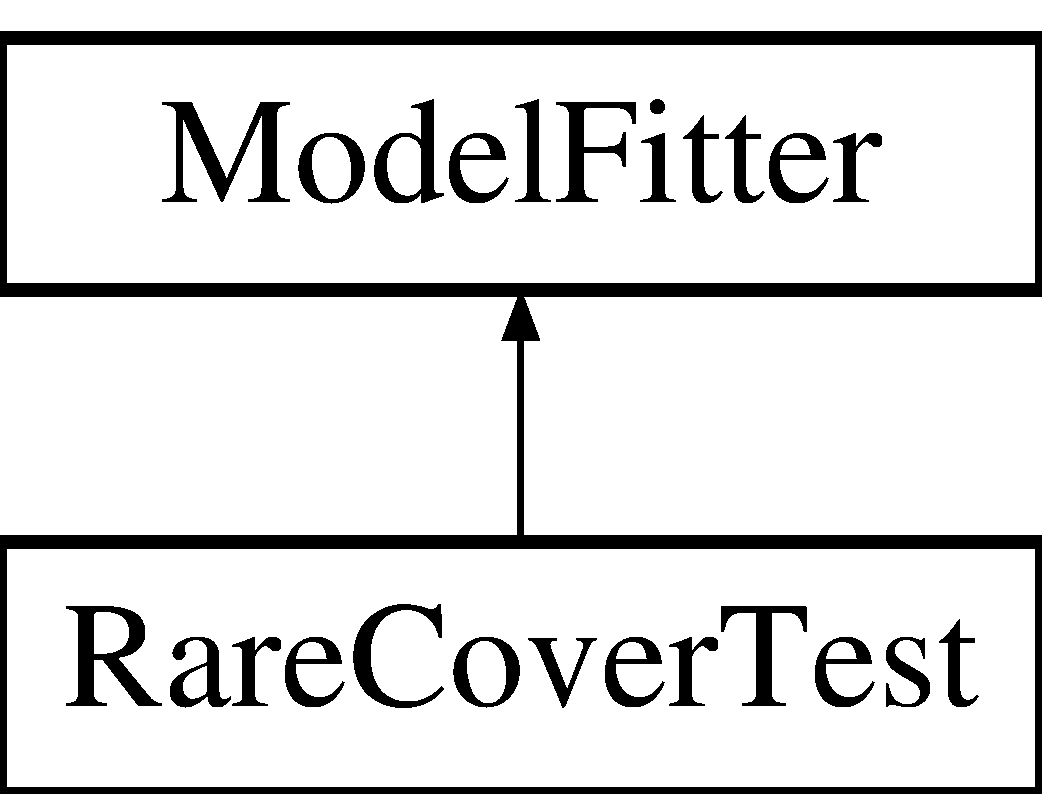
\includegraphics[height=2.000000cm]{classRareCoverTest}
\end{center}
\end{figure}
\subsection*{Public Member Functions}
\begin{DoxyCompactItemize}
\item 
\hypertarget{classRareCoverTest_a65a7be8d4f72226c2e378251a1110642}{{\bfseries Rare\-Cover\-Test} (int n\-Perm, double alpha)}\label{classRareCoverTest_a65a7be8d4f72226c2e378251a1110642}

\item 
\hypertarget{classRareCoverTest_a0c3dd9692b804f5c9ba712fb195161f9}{int {\bfseries fit} (\hyperlink{classDataConsolidator}{Data\-Consolidator} $\ast$dc)}\label{classRareCoverTest_a0c3dd9692b804f5c9ba712fb195161f9}

\item 
\hypertarget{classRareCoverTest_a78626327132047575b9c36f6f0dc5e5f}{void {\bfseries reset} ()}\label{classRareCoverTest_a78626327132047575b9c36f6f0dc5e5f}

\item 
\hypertarget{classRareCoverTest_a2d8d5fd3d311e773b6f974dc6e796b63}{void {\bfseries write\-Header} (File\-Writer $\ast$fp, const \hyperlink{classResult}{Result} \&site\-Info)}\label{classRareCoverTest_a2d8d5fd3d311e773b6f974dc6e796b63}

\item 
\hypertarget{classRareCoverTest_a1af6aae137c2a322f6e7a309bcf67b20}{void {\bfseries write\-Output} (File\-Writer $\ast$fp, const \hyperlink{classResult}{Result} \&site\-Info)}\label{classRareCoverTest_a1af6aae137c2a322f6e7a309bcf67b20}

\item 
double \hyperlink{classRareCoverTest_a425080e90820f33773da8111b641f053}{calculate\-Stat} (Matrix \&genotype, Vector \&phenotype, std\-::set$<$ int $>$ $\ast$selected\-Index)
\item 
double \hyperlink{classRareCoverTest_acbebef2b77dba2dc49eb75ead9425668}{calculate\-Correlation} (Vector \&g, Vector \&collapsed, Vector \&pheno)
\item 
\hypertarget{classRareCoverTest_aa8aeb38d2968517510407a103d7cbaf0}{void {\bfseries combine} (Vector $\ast$c, Vector \&v)}\label{classRareCoverTest_aa8aeb38d2968517510407a103d7cbaf0}

\end{DoxyCompactItemize}
\subsection*{Additional Inherited Members}


\subsection{Member Function Documentation}
\hypertarget{classRareCoverTest_acbebef2b77dba2dc49eb75ead9425668}{\index{Rare\-Cover\-Test@{Rare\-Cover\-Test}!calculate\-Correlation@{calculate\-Correlation}}
\index{calculate\-Correlation@{calculate\-Correlation}!RareCoverTest@{Rare\-Cover\-Test}}
\subsubsection[{calculate\-Correlation}]{\setlength{\rightskip}{0pt plus 5cm}double Rare\-Cover\-Test\-::calculate\-Correlation (
\begin{DoxyParamCaption}
\item[{Vector \&}]{g, }
\item[{Vector \&}]{collapsed, }
\item[{Vector \&}]{pheno}
\end{DoxyParamCaption}
)\hspace{0.3cm}{\ttfamily [inline]}}}\label{classRareCoverTest_acbebef2b77dba2dc49eb75ead9425668}
Calculate correlatio of (g + collapsed, pheno) \hypertarget{classRareCoverTest_a425080e90820f33773da8111b641f053}{\index{Rare\-Cover\-Test@{Rare\-Cover\-Test}!calculate\-Stat@{calculate\-Stat}}
\index{calculate\-Stat@{calculate\-Stat}!RareCoverTest@{Rare\-Cover\-Test}}
\subsubsection[{calculate\-Stat}]{\setlength{\rightskip}{0pt plus 5cm}double Rare\-Cover\-Test\-::calculate\-Stat (
\begin{DoxyParamCaption}
\item[{Matrix \&}]{genotype, }
\item[{Vector \&}]{phenotype, }
\item[{std\-::set$<$ int $>$ $\ast$}]{selected\-Index}
\end{DoxyParamCaption}
)\hspace{0.3cm}{\ttfamily [inline]}}}\label{classRareCoverTest_a425080e90820f33773da8111b641f053}
For a given genotype and phenotype, calculate Rare\-Cover stats, which markers are selected Here the genotype is\-: marker by people 

The documentation for this class was generated from the following file\-:\begin{DoxyCompactItemize}
\item 
Model\-Fitter.\-h\end{DoxyCompactItemize}

\hypertarget{classResult}{\section{Result Class Reference}
\label{classResult}\index{Result@{Result}}
}


{\ttfamily \#include $<$Result.\-h$>$}

\subsection*{Public Member Functions}
\begin{DoxyCompactItemize}
\item 
\hypertarget{classResult_a0f63b072d7567f84134ffcec3a924f2a}{void {\bfseries add\-Header} (const char $\ast$key)}\label{classResult_a0f63b072d7567f84134ffcec3a924f2a}

\item 
\hypertarget{classResult_a87c00e9ed537c49dcef0685dae7ec9dc}{void {\bfseries add\-Header} (const std\-::string \&key)}\label{classResult_a87c00e9ed537c49dcef0685dae7ec9dc}

\item 
\hypertarget{classResult_a50cb5f518e5ca57b014b9d0573adb4d5}{bool {\bfseries exist\-Header} (const char $\ast$key)}\label{classResult_a50cb5f518e5ca57b014b9d0573adb4d5}

\item 
\hypertarget{classResult_a1ff6471da8b9a1b0130590c3e590db6d}{bool {\bfseries exist\-Header} (const std\-::string \&key)}\label{classResult_a1ff6471da8b9a1b0130590c3e590db6d}

\item 
\hypertarget{classResult_a10a69516ab8591397f866cad16c7a61d}{void {\bfseries update\-Value} (const char $\ast$key, const char $\ast$val)}\label{classResult_a10a69516ab8591397f866cad16c7a61d}

\item 
\hypertarget{classResult_a78a0b995f32f4d24baea05cf6a9af4f4}{void {\bfseries update\-Value} (const char $\ast$key, const std\-::string \&val)}\label{classResult_a78a0b995f32f4d24baea05cf6a9af4f4}

\item 
\hypertarget{classResult_afb4a534e62e3d40a8361fe2ecd4d920a}{void {\bfseries update\-Value} (const std\-::string \&key, const std\-::string \&val)}\label{classResult_afb4a534e62e3d40a8361fe2ecd4d920a}

\item 
\hypertarget{classResult_aa89d84fbcf87eae1d61a5b1b039aa007}{void {\bfseries update\-Value} (const char $\ast$key, const int val)}\label{classResult_aa89d84fbcf87eae1d61a5b1b039aa007}

\item 
\hypertarget{classResult_a2206ecba5c14edaf1d63a4074cd2e8f5}{void {\bfseries update\-Value} (const char $\ast$key, const double val)}\label{classResult_a2206ecba5c14edaf1d63a4074cd2e8f5}

\item 
\hypertarget{classResult_a153c42696b148e9ad7ebd201925946b3}{void {\bfseries clear\-Value} ()}\label{classResult_a153c42696b148e9ad7ebd201925946b3}

\item 
void \hyperlink{classResult_a92602a917ef47a87fdc16762d0017f3c}{write\-Header} (F\-I\-L\-E $\ast$fp) const 
\item 
\hypertarget{classResult_a212d4d6000439de7a1cec04e9b110f01}{void {\bfseries write\-Header\-Tab} (F\-I\-L\-E $\ast$fp) const }\label{classResult_a212d4d6000439de7a1cec04e9b110f01}

\item 
\hypertarget{classResult_ada699a3e8df0b0f64893ae1c25d3396c}{void {\bfseries write\-Header\-Line} (F\-I\-L\-E $\ast$fp) const }\label{classResult_ada699a3e8df0b0f64893ae1c25d3396c}

\item 
void \hyperlink{classResult_a6d61b480bc41160b47965e60c15252d4}{write\-Value} (F\-I\-L\-E $\ast$fp) const 
\item 
\hypertarget{classResult_a87a2a874ad657ed3dd539ac7e2b03cf7}{void {\bfseries write\-Value\-Tab} (F\-I\-L\-E $\ast$fp) const }\label{classResult_a87a2a874ad657ed3dd539ac7e2b03cf7}

\item 
\hypertarget{classResult_a69d2a73528e2c8f7c00f99ac6de63eb1}{void {\bfseries write\-Value\-Line} (F\-I\-L\-E $\ast$fp) const }\label{classResult_a69d2a73528e2c8f7c00f99ac6de63eb1}

\item 
void \hyperlink{classResult_ab8bf57bfefe1d12a45dbee6fc6d93401}{write\-Header} (File\-Writer $\ast$fp) const 
\item 
\hypertarget{classResult_ab6269f3e81b219782a17bb14e1873dd2}{void {\bfseries write\-Header\-Tab} (File\-Writer $\ast$fp) const }\label{classResult_ab6269f3e81b219782a17bb14e1873dd2}

\item 
\hypertarget{classResult_aa58493ead62143258d7ee80472dd8454}{void {\bfseries write\-Header\-Line} (File\-Writer $\ast$fp) const }\label{classResult_aa58493ead62143258d7ee80472dd8454}

\item 
void \hyperlink{classResult_a4edcccab48b157e081ac1a63090848ce}{write\-Value} (File\-Writer $\ast$fp) const 
\item 
\hypertarget{classResult_a19f1cfee0a96b6379c5d055f577563f2}{void {\bfseries write\-Value\-Tab} (File\-Writer $\ast$fp) const }\label{classResult_a19f1cfee0a96b6379c5d055f577563f2}

\item 
\hypertarget{classResult_a7dde3225ef12295468dcd94e536fd3d5}{void {\bfseries write\-Value\-Line} (File\-Writer $\ast$fp) const }\label{classResult_a7dde3225ef12295468dcd94e536fd3d5}

\item 
std\-::string \hyperlink{classResult_a3fb648ffdefe96e7ffc00a2a294d89f3}{join\-Header} () const 
\item 
\hypertarget{classResult_ad4e01fb1cbc1b2251037f3616e3202bc}{std\-::string {\bfseries join\-Value} (const char c= '\textbackslash{}t') const }\label{classResult_ad4e01fb1cbc1b2251037f3616e3202bc}

\item 
\hypertarget{classResult_a455408961e4ec9b7c7a162f2695842a2}{const std\-::string \& {\bfseries operator\mbox{[}$\,$\mbox{]}} (const std\-::string \&key) const }\label{classResult_a455408961e4ec9b7c7a162f2695842a2}

\item 
\hypertarget{classResult_a2302fdfaabc24530943795ae7c488ae4}{const std\-::string \& {\bfseries operator\mbox{[}$\,$\mbox{]}} (const char $\ast$key) const }\label{classResult_a2302fdfaabc24530943795ae7c488ae4}

\end{DoxyCompactItemize}


\subsection{Detailed Description}
Store key-\/value pair for minimal typing Internally, all keys and values are strings Memory layout\-: key1 -\/$>$ val, val, val.... key2 -\/$>$ val, val, val.... $^\wedge$ $^\wedge$ $^\wedge$ $|$ $|$ $|$ L1 L2 L3 We assume updating data are performed layer by layer If cross layout updating value happened, we will generate an error. 

\subsection{Member Function Documentation}
\hypertarget{classResult_a3fb648ffdefe96e7ffc00a2a294d89f3}{\index{Result@{Result}!join\-Header@{join\-Header}}
\index{join\-Header@{join\-Header}!Result@{Result}}
\subsubsection[{join\-Header}]{\setlength{\rightskip}{0pt plus 5cm}std\-::string Result\-::join\-Header (
\begin{DoxyParamCaption}
{}
\end{DoxyParamCaption}
) const\hspace{0.3cm}{\ttfamily [inline]}}}\label{classResult_a3fb648ffdefe96e7ffc00a2a294d89f3}
Use '' to join headers \hypertarget{classResult_a92602a917ef47a87fdc16762d0017f3c}{\index{Result@{Result}!write\-Header@{write\-Header}}
\index{write\-Header@{write\-Header}!Result@{Result}}
\subsubsection[{write\-Header}]{\setlength{\rightskip}{0pt plus 5cm}void Result\-::write\-Header (
\begin{DoxyParamCaption}
\item[{F\-I\-L\-E $\ast$}]{fp}
\end{DoxyParamCaption}
) const\hspace{0.3cm}{\ttfamily [inline]}}}\label{classResult_a92602a917ef47a87fdc16762d0017f3c}
Write the keys separated by '' \hypertarget{classResult_ab8bf57bfefe1d12a45dbee6fc6d93401}{\index{Result@{Result}!write\-Header@{write\-Header}}
\index{write\-Header@{write\-Header}!Result@{Result}}
\subsubsection[{write\-Header}]{\setlength{\rightskip}{0pt plus 5cm}void Result\-::write\-Header (
\begin{DoxyParamCaption}
\item[{File\-Writer $\ast$}]{fp}
\end{DoxyParamCaption}
) const\hspace{0.3cm}{\ttfamily [inline]}}}\label{classResult_ab8bf57bfefe1d12a45dbee6fc6d93401}
Write the keys separated by '' \hypertarget{classResult_a6d61b480bc41160b47965e60c15252d4}{\index{Result@{Result}!write\-Value@{write\-Value}}
\index{write\-Value@{write\-Value}!Result@{Result}}
\subsubsection[{write\-Value}]{\setlength{\rightskip}{0pt plus 5cm}void Result\-::write\-Value (
\begin{DoxyParamCaption}
\item[{F\-I\-L\-E $\ast$}]{fp}
\end{DoxyParamCaption}
) const\hspace{0.3cm}{\ttfamily [inline]}}}\label{classResult_a6d61b480bc41160b47965e60c15252d4}
Write the values separated by '' \hypertarget{classResult_a4edcccab48b157e081ac1a63090848ce}{\index{Result@{Result}!write\-Value@{write\-Value}}
\index{write\-Value@{write\-Value}!Result@{Result}}
\subsubsection[{write\-Value}]{\setlength{\rightskip}{0pt plus 5cm}void Result\-::write\-Value (
\begin{DoxyParamCaption}
\item[{File\-Writer $\ast$}]{fp}
\end{DoxyParamCaption}
) const\hspace{0.3cm}{\ttfamily [inline]}}}\label{classResult_a4edcccab48b157e081ac1a63090848ce}
Write the values separated by '' 

The documentation for this class was generated from the following file\-:\begin{DoxyCompactItemize}
\item 
Result.\-h\end{DoxyCompactItemize}

\hypertarget{classSingleVariantFamilyGrammarGamma}{\section{Single\-Variant\-Family\-Grammar\-Gamma Class Reference}
\label{classSingleVariantFamilyGrammarGamma}\index{Single\-Variant\-Family\-Grammar\-Gamma@{Single\-Variant\-Family\-Grammar\-Gamma}}
}
Inheritance diagram for Single\-Variant\-Family\-Grammar\-Gamma\-:\begin{figure}[H]
\begin{center}
\leavevmode
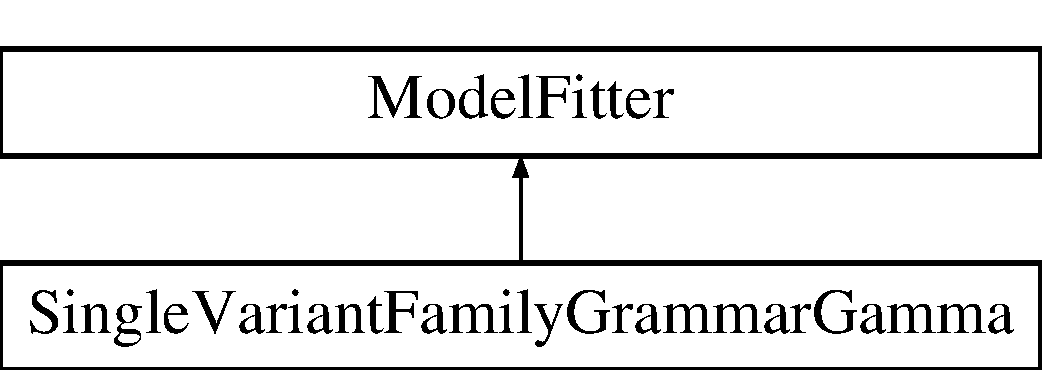
\includegraphics[height=2.000000cm]{classSingleVariantFamilyGrammarGamma}
\end{center}
\end{figure}
\subsection*{Public Member Functions}
\begin{DoxyCompactItemize}
\item 
\hypertarget{classSingleVariantFamilyGrammarGamma_a3868ad08b97521ee952022bd31fef164}{int {\bfseries fit} (\hyperlink{classDataConsolidator}{Data\-Consolidator} $\ast$dc)}\label{classSingleVariantFamilyGrammarGamma_a3868ad08b97521ee952022bd31fef164}

\item 
\hypertarget{classSingleVariantFamilyGrammarGamma_ac5a1e16454019e83fe65382c695c4b4d}{void {\bfseries write\-Header} (File\-Writer $\ast$fp, const \hyperlink{classResult}{Result} \&site\-Info)}\label{classSingleVariantFamilyGrammarGamma_ac5a1e16454019e83fe65382c695c4b4d}

\item 
\hypertarget{classSingleVariantFamilyGrammarGamma_a5d3d41d262a4d627b7b87f0f7d0d4a1c}{void {\bfseries write\-Output} (File\-Writer $\ast$fp, const \hyperlink{classResult}{Result} \&site\-Info)}\label{classSingleVariantFamilyGrammarGamma_a5d3d41d262a4d627b7b87f0f7d0d4a1c}

\item 
\hypertarget{classSingleVariantFamilyGrammarGamma_aefda5b739ddb46c46db64d604c01202b}{void {\bfseries write\-Footnote} (File\-Writer $\ast$fp)}\label{classSingleVariantFamilyGrammarGamma_aefda5b739ddb46c46db64d604c01202b}

\end{DoxyCompactItemize}
\subsection*{Additional Inherited Members}


The documentation for this class was generated from the following file\-:\begin{DoxyCompactItemize}
\item 
Model\-Fitter.\-h\end{DoxyCompactItemize}

\hypertarget{classSingleVariantFamilyLRT}{\section{Single\-Variant\-Family\-L\-R\-T Class Reference}
\label{classSingleVariantFamilyLRT}\index{Single\-Variant\-Family\-L\-R\-T@{Single\-Variant\-Family\-L\-R\-T}}
}
Inheritance diagram for Single\-Variant\-Family\-L\-R\-T\-:\begin{figure}[H]
\begin{center}
\leavevmode
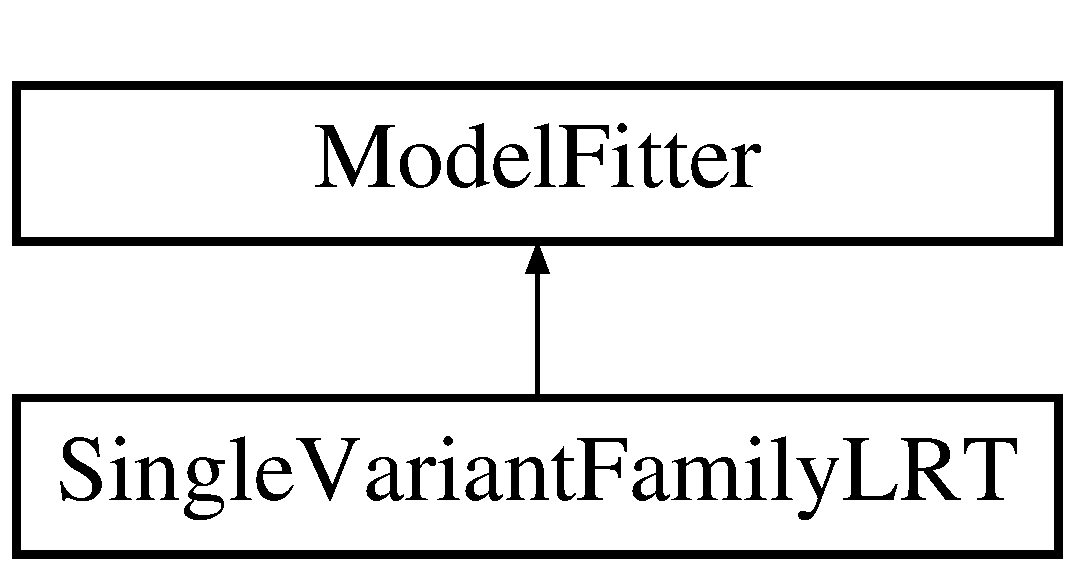
\includegraphics[height=2.000000cm]{classSingleVariantFamilyLRT}
\end{center}
\end{figure}
\subsection*{Public Member Functions}
\begin{DoxyCompactItemize}
\item 
\hypertarget{classSingleVariantFamilyLRT_a978f11d55a6efa641b8f6569510724bb}{int {\bfseries fit} (\hyperlink{classDataConsolidator}{Data\-Consolidator} $\ast$dc)}\label{classSingleVariantFamilyLRT_a978f11d55a6efa641b8f6569510724bb}

\item 
\hypertarget{classSingleVariantFamilyLRT_a388c6c566115b7f062d0d0d316a212b3}{void {\bfseries write\-Header} (File\-Writer $\ast$fp, const \hyperlink{classResult}{Result} \&site\-Info)}\label{classSingleVariantFamilyLRT_a388c6c566115b7f062d0d0d316a212b3}

\item 
\hypertarget{classSingleVariantFamilyLRT_a455598e22c24fe167ac332b689de6b3a}{void {\bfseries write\-Output} (File\-Writer $\ast$fp, const \hyperlink{classResult}{Result} \&site\-Info)}\label{classSingleVariantFamilyLRT_a455598e22c24fe167ac332b689de6b3a}

\item 
\hypertarget{classSingleVariantFamilyLRT_a7af5487044ce3a446cc8ce6b2b29171a}{void {\bfseries write\-Footnote} (File\-Writer $\ast$fp)}\label{classSingleVariantFamilyLRT_a7af5487044ce3a446cc8ce6b2b29171a}

\end{DoxyCompactItemize}
\subsection*{Additional Inherited Members}


The documentation for this class was generated from the following file\-:\begin{DoxyCompactItemize}
\item 
Model\-Fitter.\-h\end{DoxyCompactItemize}

\hypertarget{classSingleVariantFamilyScore}{\section{Single\-Variant\-Family\-Score Class Reference}
\label{classSingleVariantFamilyScore}\index{Single\-Variant\-Family\-Score@{Single\-Variant\-Family\-Score}}
}
Inheritance diagram for Single\-Variant\-Family\-Score\-:\begin{figure}[H]
\begin{center}
\leavevmode
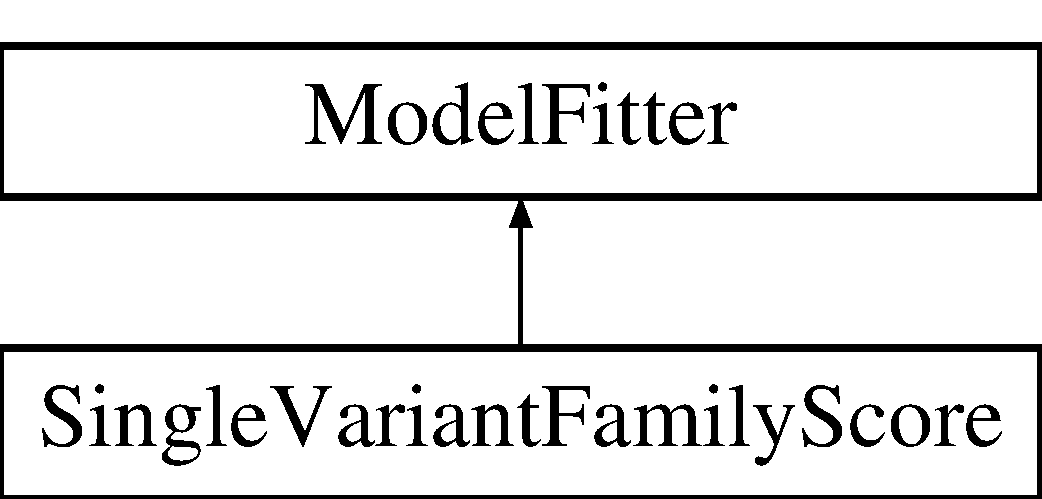
\includegraphics[height=2.000000cm]{classSingleVariantFamilyScore}
\end{center}
\end{figure}
\subsection*{Public Member Functions}
\begin{DoxyCompactItemize}
\item 
\hypertarget{classSingleVariantFamilyScore_ae63cc2219132c16d37e84a22696c8bb9}{int {\bfseries fit} (\hyperlink{classDataConsolidator}{Data\-Consolidator} $\ast$dc)}\label{classSingleVariantFamilyScore_ae63cc2219132c16d37e84a22696c8bb9}

\item 
\hypertarget{classSingleVariantFamilyScore_adb1cf278e977ceafac034827a313aa5d}{void {\bfseries write\-Header} (File\-Writer $\ast$fp, const \hyperlink{classResult}{Result} \&site\-Info)}\label{classSingleVariantFamilyScore_adb1cf278e977ceafac034827a313aa5d}

\item 
\hypertarget{classSingleVariantFamilyScore_a8f38cf774a4f6c5d9f671f05f4ce2514}{void {\bfseries write\-Output} (File\-Writer $\ast$fp, const \hyperlink{classResult}{Result} \&site\-Info)}\label{classSingleVariantFamilyScore_a8f38cf774a4f6c5d9f671f05f4ce2514}

\item 
\hypertarget{classSingleVariantFamilyScore_abac2194d76b94db451c987f5d6736e81}{void {\bfseries write\-Footnote} (File\-Writer $\ast$fp)}\label{classSingleVariantFamilyScore_abac2194d76b94db451c987f5d6736e81}

\end{DoxyCompactItemize}
\subsection*{Additional Inherited Members}


The documentation for this class was generated from the following file\-:\begin{DoxyCompactItemize}
\item 
Model\-Fitter.\-h\end{DoxyCompactItemize}

\hypertarget{classSingleVariantFirthTest}{\section{Single\-Variant\-Firth\-Test Class Reference}
\label{classSingleVariantFirthTest}\index{Single\-Variant\-Firth\-Test@{Single\-Variant\-Firth\-Test}}
}
Inheritance diagram for Single\-Variant\-Firth\-Test\-:\begin{figure}[H]
\begin{center}
\leavevmode
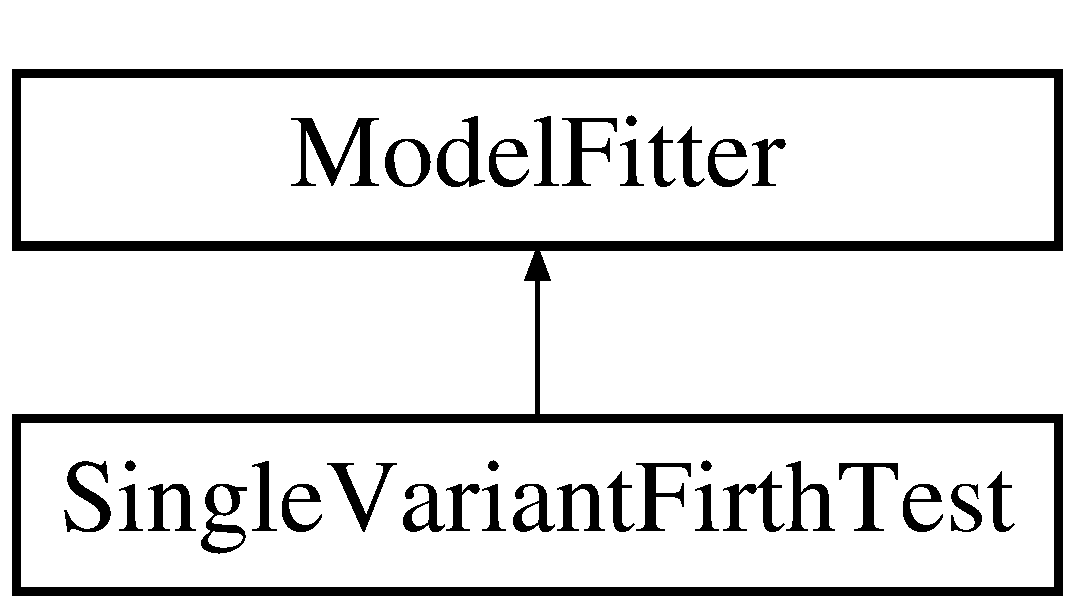
\includegraphics[height=2.000000cm]{classSingleVariantFirthTest}
\end{center}
\end{figure}
\subsection*{Public Member Functions}
\begin{DoxyCompactItemize}
\item 
\hypertarget{classSingleVariantFirthTest_a43fb9b330b4634ebb1051ec5fac81a56}{int {\bfseries fit} (\hyperlink{classDataConsolidator}{Data\-Consolidator} $\ast$dc)}\label{classSingleVariantFirthTest_a43fb9b330b4634ebb1051ec5fac81a56}

\item 
\hypertarget{classSingleVariantFirthTest_ad74ecdd1516432bacb7ac7d617cc007e}{void {\bfseries write\-Header} (File\-Writer $\ast$fp, const \hyperlink{classResult}{Result} \&site\-Info)}\label{classSingleVariantFirthTest_ad74ecdd1516432bacb7ac7d617cc007e}

\item 
\hypertarget{classSingleVariantFirthTest_adfcd926da6a84ae788f1165177bfc455}{void {\bfseries write\-Output} (File\-Writer $\ast$fp, const \hyperlink{classResult}{Result} \&site\-Info)}\label{classSingleVariantFirthTest_adfcd926da6a84ae788f1165177bfc455}

\end{DoxyCompactItemize}
\subsection*{Additional Inherited Members}


The documentation for this class was generated from the following file\-:\begin{DoxyCompactItemize}
\item 
Model\-Fitter.\-h\end{DoxyCompactItemize}

\hypertarget{classSingleVariantFisherExactTest}{\section{Single\-Variant\-Fisher\-Exact\-Test Class Reference}
\label{classSingleVariantFisherExactTest}\index{Single\-Variant\-Fisher\-Exact\-Test@{Single\-Variant\-Fisher\-Exact\-Test}}
}
Inheritance diagram for Single\-Variant\-Fisher\-Exact\-Test\-:\begin{figure}[H]
\begin{center}
\leavevmode
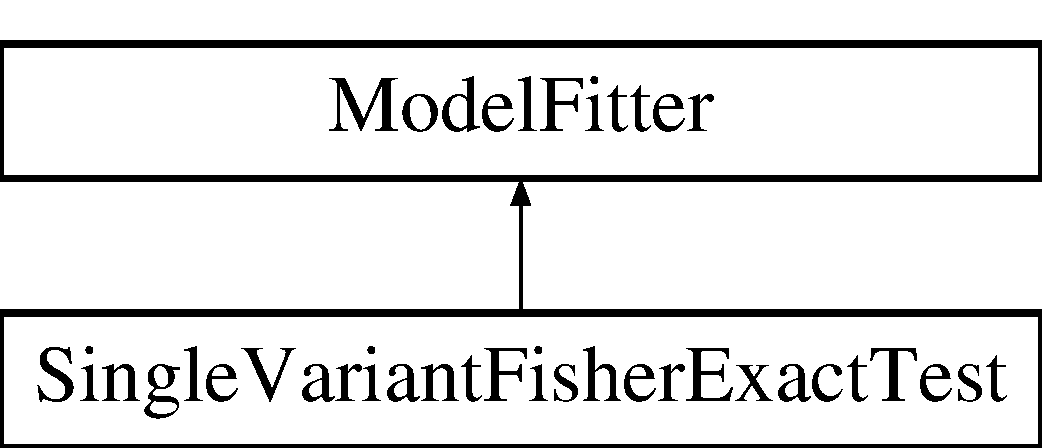
\includegraphics[height=2.000000cm]{classSingleVariantFisherExactTest}
\end{center}
\end{figure}
\subsection*{Public Member Functions}
\begin{DoxyCompactItemize}
\item 
\hypertarget{classSingleVariantFisherExactTest_ac67f9a9f1d0ce580c1885af46f77e67e}{void {\bfseries write\-Header} (File\-Writer $\ast$fp, const \hyperlink{classResult}{Result} \&site\-Info)}\label{classSingleVariantFisherExactTest_ac67f9a9f1d0ce580c1885af46f77e67e}

\item 
\hypertarget{classSingleVariantFisherExactTest_ab746bc0d0464efab94f2369aa424027c}{int {\bfseries fit} (\hyperlink{classDataConsolidator}{Data\-Consolidator} $\ast$dc)}\label{classSingleVariantFisherExactTest_ab746bc0d0464efab94f2369aa424027c}

\item 
\hypertarget{classSingleVariantFisherExactTest_ac6515494462e8508a746bd1b28b65554}{void {\bfseries write\-Output} (File\-Writer $\ast$fp, const \hyperlink{classResult}{Result} \&site\-Info)}\label{classSingleVariantFisherExactTest_ac6515494462e8508a746bd1b28b65554}

\item 
\hypertarget{classSingleVariantFisherExactTest_a2380094c14667313baf3fcbf28a48ac9}{void {\bfseries reset} ()}\label{classSingleVariantFisherExactTest_a2380094c14667313baf3fcbf28a48ac9}

\end{DoxyCompactItemize}
\subsection*{Additional Inherited Members}


The documentation for this class was generated from the following file\-:\begin{DoxyCompactItemize}
\item 
Model\-Fitter.\-h\end{DoxyCompactItemize}

\hypertarget{classSingleVariantScoreTest}{\section{Single\-Variant\-Score\-Test Class Reference}
\label{classSingleVariantScoreTest}\index{Single\-Variant\-Score\-Test@{Single\-Variant\-Score\-Test}}
}
Inheritance diagram for Single\-Variant\-Score\-Test\-:\begin{figure}[H]
\begin{center}
\leavevmode
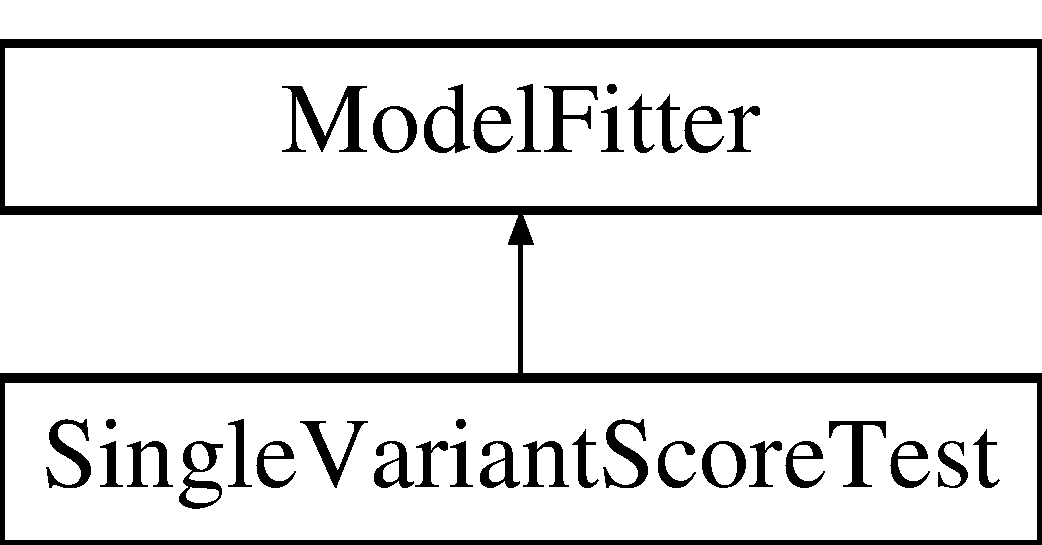
\includegraphics[height=2.000000cm]{classSingleVariantScoreTest}
\end{center}
\end{figure}
\subsection*{Public Member Functions}
\begin{DoxyCompactItemize}
\item 
\hypertarget{classSingleVariantScoreTest_aba86a76f5311030a97493a6ebcb83697}{int {\bfseries fit} (\hyperlink{classDataConsolidator}{Data\-Consolidator} $\ast$dc)}\label{classSingleVariantScoreTest_aba86a76f5311030a97493a6ebcb83697}

\item 
\hypertarget{classSingleVariantScoreTest_a11c16becc464c6796b3b898004bd8d5f}{void {\bfseries write\-Header} (File\-Writer $\ast$fp, const \hyperlink{classResult}{Result} \&site\-Info)}\label{classSingleVariantScoreTest_a11c16becc464c6796b3b898004bd8d5f}

\item 
\hypertarget{classSingleVariantScoreTest_a628b4a6c5c00841df6658bc0e48f87ee}{void {\bfseries write\-Output} (File\-Writer $\ast$fp, const \hyperlink{classResult}{Result} \&site\-Info)}\label{classSingleVariantScoreTest_a628b4a6c5c00841df6658bc0e48f87ee}

\end{DoxyCompactItemize}
\subsection*{Additional Inherited Members}


The documentation for this class was generated from the following file\-:\begin{DoxyCompactItemize}
\item 
Model\-Fitter.\-h\end{DoxyCompactItemize}

\hypertarget{classSingleVariantWaldTest}{\section{Single\-Variant\-Wald\-Test Class Reference}
\label{classSingleVariantWaldTest}\index{Single\-Variant\-Wald\-Test@{Single\-Variant\-Wald\-Test}}
}
Inheritance diagram for Single\-Variant\-Wald\-Test\-:\begin{figure}[H]
\begin{center}
\leavevmode
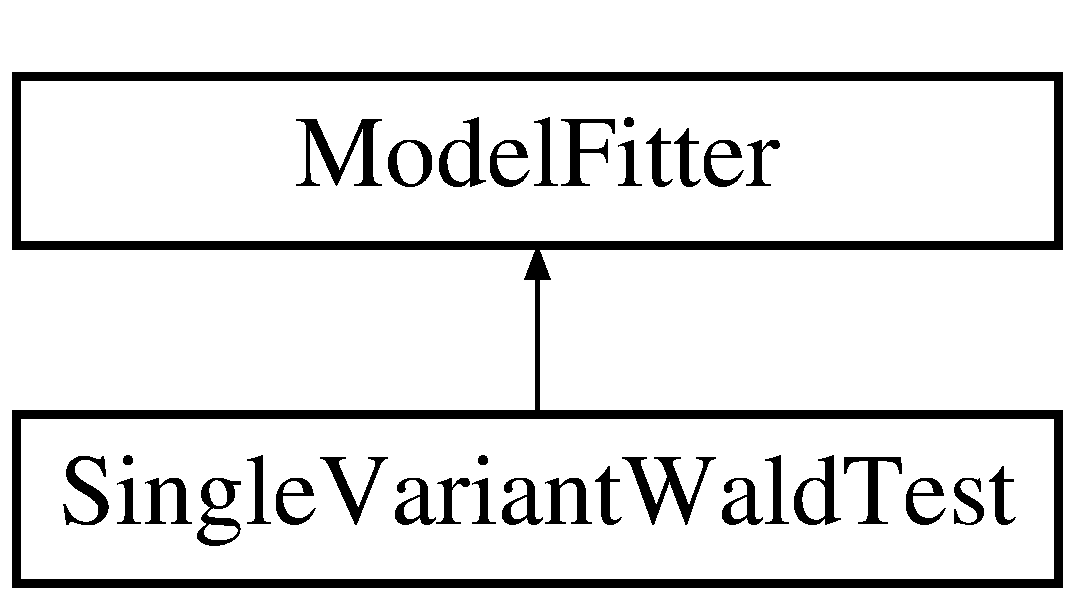
\includegraphics[height=2.000000cm]{classSingleVariantWaldTest}
\end{center}
\end{figure}
\subsection*{Public Member Functions}
\begin{DoxyCompactItemize}
\item 
\hypertarget{classSingleVariantWaldTest_a5ebe41360afa081a20d2daf4ec6d5eee}{int {\bfseries fit} (\hyperlink{classDataConsolidator}{Data\-Consolidator} $\ast$dc)}\label{classSingleVariantWaldTest_a5ebe41360afa081a20d2daf4ec6d5eee}

\item 
\hypertarget{classSingleVariantWaldTest_a25129546a6d70790213cf925a675691a}{void {\bfseries write\-Header} (File\-Writer $\ast$fp, const \hyperlink{classResult}{Result} \&site\-Info)}\label{classSingleVariantWaldTest_a25129546a6d70790213cf925a675691a}

\item 
\hypertarget{classSingleVariantWaldTest_afad368d8a7ab642e64260c4fe9daaf9a}{void {\bfseries write\-Output} (File\-Writer $\ast$fp, const \hyperlink{classResult}{Result} \&site\-Info)}\label{classSingleVariantWaldTest_afad368d8a7ab642e64260c4fe9daaf9a}

\end{DoxyCompactItemize}
\subsection*{Additional Inherited Members}


The documentation for this class was generated from the following file\-:\begin{DoxyCompactItemize}
\item 
Model\-Fitter.\-h\end{DoxyCompactItemize}

\hypertarget{classSkatTest}{\section{Skat\-Test Class Reference}
\label{classSkatTest}\index{Skat\-Test@{Skat\-Test}}
}
Inheritance diagram for Skat\-Test\-:\begin{figure}[H]
\begin{center}
\leavevmode
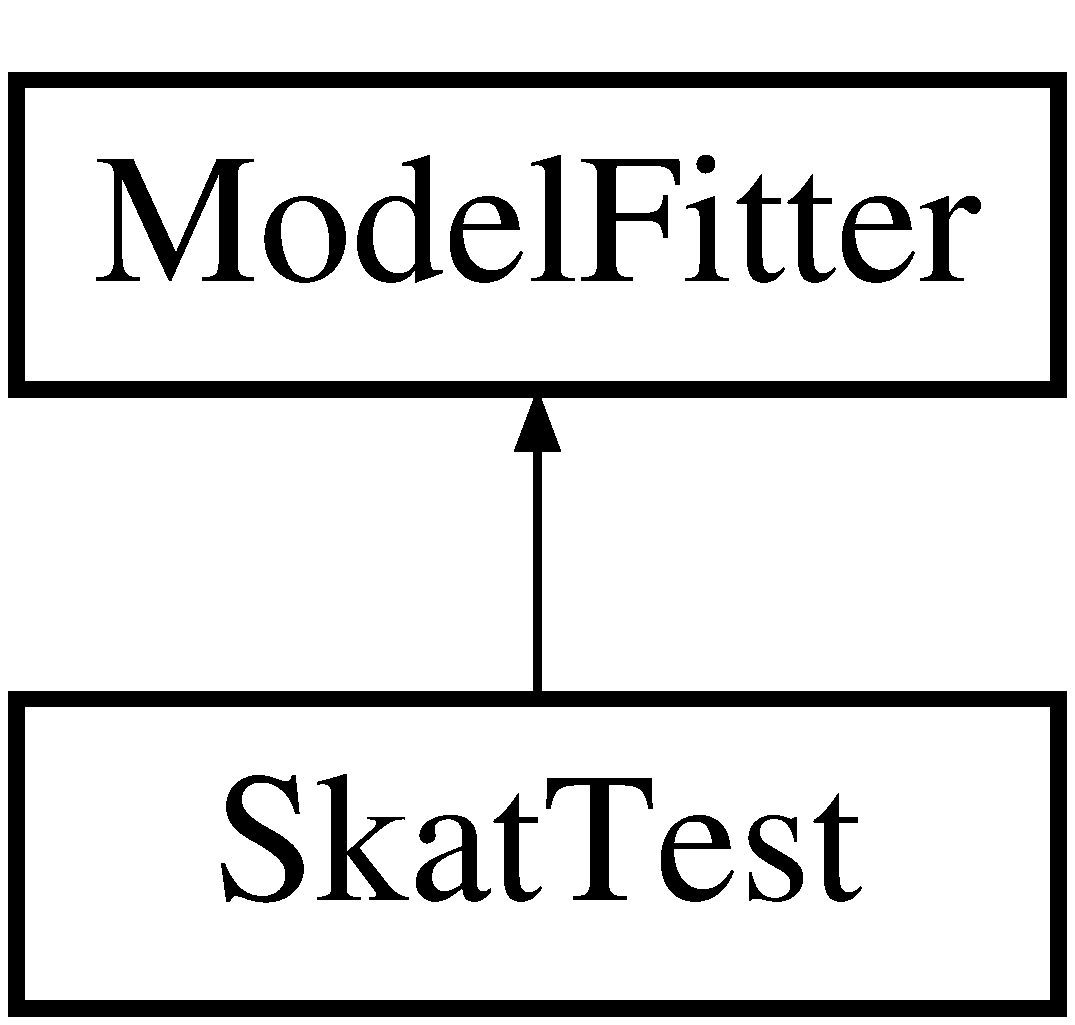
\includegraphics[height=2.000000cm]{classSkatTest}
\end{center}
\end{figure}
\subsection*{Public Member Functions}
\begin{DoxyCompactItemize}
\item 
\hypertarget{classSkatTest_af780a3f263eb12f976ec8d1528e09eba}{{\bfseries Skat\-Test} (int n\-Perm, double alpha, double beta1, double beta2)}\label{classSkatTest_af780a3f263eb12f976ec8d1528e09eba}

\item 
\hypertarget{classSkatTest_a6ce75617c1e0e4d63e6bd95415dbe431}{void {\bfseries reset} ()}\label{classSkatTest_a6ce75617c1e0e4d63e6bd95415dbe431}

\item 
int \hyperlink{classSkatTest_a7cf069d7bf19a2d6f238f14518f69ebe}{fit} (\hyperlink{classDataConsolidator}{Data\-Consolidator} $\ast$dc)
\item 
\hypertarget{classSkatTest_aaf1c103dac2289666011fd64c3b2de25}{void {\bfseries write\-Header} (File\-Writer $\ast$fp, const \hyperlink{classResult}{Result} \&site\-Info)}\label{classSkatTest_aaf1c103dac2289666011fd64c3b2de25}

\item 
\hypertarget{classSkatTest_a780ba3fded4d1bf77d00bd8f33ddf5be}{void {\bfseries write\-Output} (File\-Writer $\ast$fp, const \hyperlink{classResult}{Result} \&site\-Info)}\label{classSkatTest_a780ba3fded4d1bf77d00bd8f33ddf5be}

\end{DoxyCompactItemize}
\subsection*{Additional Inherited Members}


\subsection{Member Function Documentation}
\hypertarget{classSkatTest_a7cf069d7bf19a2d6f238f14518f69ebe}{\index{Skat\-Test@{Skat\-Test}!fit@{fit}}
\index{fit@{fit}!SkatTest@{Skat\-Test}}
\subsubsection[{fit}]{\setlength{\rightskip}{0pt plus 5cm}int Skat\-Test\-::fit (
\begin{DoxyParamCaption}
\item[{{\bf Data\-Consolidator} $\ast$}]{dc}
\end{DoxyParamCaption}
)\hspace{0.3cm}{\ttfamily [inline]}, {\ttfamily [virtual]}}}\label{classSkatTest_a7cf069d7bf19a2d6f238f14518f69ebe}
default S\-K\-A\-T use beta(\-M\-A\-F, 1, 25) 

Implements \hyperlink{classModelFitter}{Model\-Fitter}.



The documentation for this class was generated from the following file\-:\begin{DoxyCompactItemize}
\item 
Model\-Fitter.\-h\end{DoxyCompactItemize}

\hypertarget{classSummary}{\section{Summary Class Reference}
\label{classSummary}\index{Summary@{Summary}}
}
\subsection*{Public Member Functions}
\begin{DoxyCompactItemize}
\item 
\hypertarget{classSummary_ae28f345fbe1ad93d827b794b794b9cdc}{void {\bfseries add} (const std\-::vector$<$ double $>$ \&v)}\label{classSummary_ae28f345fbe1ad93d827b794b794b9cdc}

\end{DoxyCompactItemize}
\subsection*{Public Attributes}
\begin{DoxyCompactItemize}
\item 
\hypertarget{classSummary_a1dddaed512bba6bb9ee05d5524957a83}{double {\bfseries min}}\label{classSummary_a1dddaed512bba6bb9ee05d5524957a83}

\item 
\hypertarget{classSummary_a9cd53f493ab67ebf72a415bfb54b1b6e}{double {\bfseries q1}}\label{classSummary_a9cd53f493ab67ebf72a415bfb54b1b6e}

\item 
\hypertarget{classSummary_ae571634b59f79bf4d542e348c9af5162}{double {\bfseries median}}\label{classSummary_ae571634b59f79bf4d542e348c9af5162}

\item 
\hypertarget{classSummary_acf4deb21b9e231bd0e06a058c7c27133}{double {\bfseries q3}}\label{classSummary_acf4deb21b9e231bd0e06a058c7c27133}

\item 
\hypertarget{classSummary_a9009a80ad03d3e04f52012a736331caa}{double {\bfseries max}}\label{classSummary_a9009a80ad03d3e04f52012a736331caa}

\item 
\hypertarget{classSummary_aa04053684b9e18daaadbad2230982216}{double {\bfseries mean}}\label{classSummary_aa04053684b9e18daaadbad2230982216}

\item 
\hypertarget{classSummary_aeca0cb835e436a26ae1fbee6dea2ebed}{double {\bfseries sd}}\label{classSummary_aeca0cb835e436a26ae1fbee6dea2ebed}

\item 
\hypertarget{classSummary_af4b5493fad630e07d86565574a5bb839}{int {\bfseries n}}\label{classSummary_af4b5493fad630e07d86565574a5bb839}

\end{DoxyCompactItemize}


The documentation for this class was generated from the following file\-:\begin{DoxyCompactItemize}
\item 
Summary.\-h\end{DoxyCompactItemize}

\hypertarget{classSummaryHeader}{\section{Summary\-Header Class Reference}
\label{classSummaryHeader}\index{Summary\-Header@{Summary\-Header}}
}


{\ttfamily \#include $<$Summary.\-h$>$}

\subsection*{Public Member Functions}
\begin{DoxyCompactItemize}
\item 
\hypertarget{classSummaryHeader_a57c66924a410e9795ca6cf10958bb289}{void {\bfseries record\-Phenotype} (const char $\ast$label, const std\-::vector$<$ double $>$ \&pheno)}\label{classSummaryHeader_a57c66924a410e9795ca6cf10958bb289}

\item 
\hypertarget{classSummaryHeader_a22a58cc4a69af535073ea29bf8296eb0}{void {\bfseries set\-Inverse\-Normalize} (bool b)}\label{classSummaryHeader_a22a58cc4a69af535073ea29bf8296eb0}

\item 
\hypertarget{classSummaryHeader_a60a5f6ff66092b8379dad2837f3bf7f1}{void {\bfseries record\-Covariate\-Column} (Matrix \&m, int col)}\label{classSummaryHeader_a60a5f6ff66092b8379dad2837f3bf7f1}

\item 
\hypertarget{classSummaryHeader_a18e781a07579955e0e7eea1b103280be}{void {\bfseries record\-Covariate} (Matrix \&m)}\label{classSummaryHeader_a18e781a07579955e0e7eea1b103280be}

\item 
\hypertarget{classSummaryHeader_a7f82d2263d52c75c5e808dc9bb317ed2}{void {\bfseries fit\-Model} (const std\-::vector$<$ double $>$ \&pheno, bool binary\-Phenotype, Matrix \&cov)}\label{classSummaryHeader_a7f82d2263d52c75c5e808dc9bb317ed2}

\item 
\hypertarget{classSummaryHeader_a3f6a9365fd0e30bb076ae61dc45dfeaf}{void {\bfseries output\-Header} (File\-Writer $\ast$fp)}\label{classSummaryHeader_a3f6a9365fd0e30bb076ae61dc45dfeaf}

\item 
\hypertarget{classSummaryHeader_a837a8fe3ca1ea37df06c35261ac19bcf}{void {\bfseries print\-Null\-Model\-Estimate} (File\-Writer $\ast$fp, const Vector \&beta, const Matrix \&beta\-Sd, const double sigma)}\label{classSummaryHeader_a837a8fe3ca1ea37df06c35261ac19bcf}

\end{DoxyCompactItemize}


\subsection{Detailed Description}
A class to summarize phenotype and genotypes 

The documentation for this class was generated from the following file\-:\begin{DoxyCompactItemize}
\item 
Summary.\-h\end{DoxyCompactItemize}

\hypertarget{classVariableThresholdPrice}{\section{Variable\-Threshold\-Price Class Reference}
\label{classVariableThresholdPrice}\index{Variable\-Threshold\-Price@{Variable\-Threshold\-Price}}
}


{\ttfamily \#include $<$Model\-Fitter.\-h$>$}

Inheritance diagram for Variable\-Threshold\-Price\-:\begin{figure}[H]
\begin{center}
\leavevmode
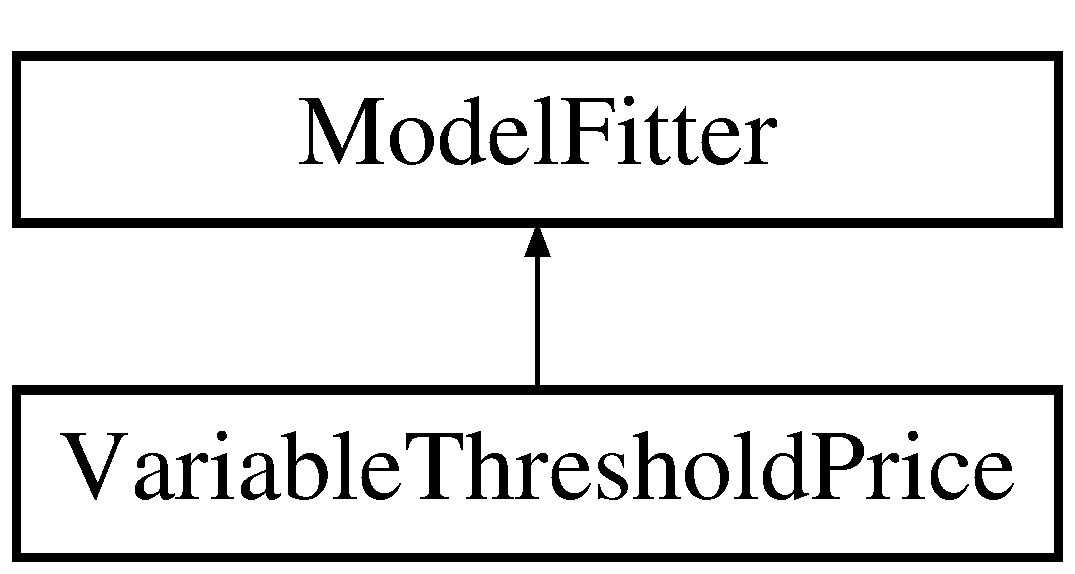
\includegraphics[height=2.000000cm]{classVariableThresholdPrice}
\end{center}
\end{figure}
\subsection*{Public Member Functions}
\begin{DoxyCompactItemize}
\item 
\hypertarget{classVariableThresholdPrice_a9fe39d3156a406c0bf1df62d0418b673}{{\bfseries Variable\-Threshold\-Price} (int n\-Perm, double alpha)}\label{classVariableThresholdPrice_a9fe39d3156a406c0bf1df62d0418b673}

\item 
\hypertarget{classVariableThresholdPrice_a6b78a3ba3b3b33f924d95f7a4631fd7b}{int {\bfseries fit} (\hyperlink{classDataConsolidator}{Data\-Consolidator} $\ast$dc)}\label{classVariableThresholdPrice_a6b78a3ba3b3b33f924d95f7a4631fd7b}

\item 
\hypertarget{classVariableThresholdPrice_ae2dd45c3b0d387bee374192ec4b54e66}{void {\bfseries write\-Header} (File\-Writer $\ast$fp, const \hyperlink{classResult}{Result} \&site\-Info)}\label{classVariableThresholdPrice_ae2dd45c3b0d387bee374192ec4b54e66}

\item 
\hypertarget{classVariableThresholdPrice_abebd5bb0e6a1f8a71849c9302f1f7c39}{void {\bfseries write\-Output} (File\-Writer $\ast$fp, const \hyperlink{classResult}{Result} \&site\-Info)}\label{classVariableThresholdPrice_abebd5bb0e6a1f8a71849c9302f1f7c39}

\item 
\hypertarget{classVariableThresholdPrice_abc9db0a117d7cc255db900a1da8cfc97}{void {\bfseries reset} ()}\label{classVariableThresholdPrice_abc9db0a117d7cc255db900a1da8cfc97}

\end{DoxyCompactItemize}
\subsection*{Additional Inherited Members}


\subsection{Detailed Description}
Implementation of Alkes Price's V\-T 

The documentation for this class was generated from the following file\-:\begin{DoxyCompactItemize}
\item 
Model\-Fitter.\-h\end{DoxyCompactItemize}

\hypertarget{classVCFData}{\section{V\-C\-F\-Data Class Reference}
\label{classVCFData}\index{V\-C\-F\-Data@{V\-C\-F\-Data}}
}


{\ttfamily \#include $<$V\-C\-F\-Data.\-h$>$}

\subsection*{Public Member Functions}
\begin{DoxyCompactItemize}
\item 
void \hyperlink{classVCFData_aa237fc9ab7baada2b1621bd098319c7e}{adjust\-People\-Order} (std\-::vector$<$ std\-::string $>$ \&p, std\-::vector$<$ std\-::string $>$ $\ast$dropped\-Id)
\item 
\hypertarget{classVCFData_a4a54a9919215f4d3ce8e7cafdc8593f4}{void {\bfseries add\-V\-C\-F\-Header} (V\-C\-F\-Header $\ast$h, std\-::vector$<$ std\-::string $>$ $\ast$dropped\-Id)}\label{classVCFData_a4a54a9919215f4d3ce8e7cafdc8593f4}

\item 
void \hyperlink{classVCFData_a5d4d267764c8fd3533242af5e11b32a2}{add\-V\-C\-F\-Record} (V\-C\-F\-Record \&r)
\item 
\hypertarget{classVCFData_a314b2f45dce69ca78a92d22e117a4680}{void {\bfseries load\-Plink} (const char $\ast$prefix)}\label{classVCFData_a314b2f45dce69ca78a92d22e117a4680}

\item 
\hypertarget{classVCFData_ac954c619485c7dde44b1d3b07df4da37}{int {\bfseries load\-Plink\-Phenotype} (const char $\ast$fn)}\label{classVCFData_ac954c619485c7dde44b1d3b07df4da37}

\item 
\hypertarget{classVCFData_afd60d597f9ea5addef895e81122c67e5}{int {\bfseries load\-Phenotype\-By\-Col} (const char $\ast$fn, int col)}\label{classVCFData_afd60d597f9ea5addef895e81122c67e5}

\item 
int \hyperlink{classVCFData_a919196e09bb6f13bcd30a313386747cd}{read\-Plink\-Phenotype\-Skip\-Missing} (const char $\ast$fn, const char $\ast$selected\-Col, Matrix $\ast$data, Ordered\-Map$<$ std\-::string, int $>$ $\ast$row\-Name, Ordered\-Map$<$ std\-::string, int $>$ $\ast$col\-Name)
\item 
\hypertarget{classVCFData_a5f33cfc1d575be6e92b9a3bd888a8057}{void {\bfseries dichotomized\-Phenotype} (double threshold)}\label{classVCFData_a5f33cfc1d575be6e92b9a3bd888a8057}

\item 
\hypertarget{classVCFData_a371f90cce2469e56d147486893fdb97e}{Vector $\ast$ {\bfseries extract\-Phenotype} ()}\label{classVCFData_a371f90cce2469e56d147486893fdb97e}

\item 
\hypertarget{classVCFData_ad2c2f810ee6ff936b62f27363921f779}{int {\bfseries load\-Covariate} (const char $\ast$fn)}\label{classVCFData_ad2c2f810ee6ff936b62f27363921f779}

\item 
\hypertarget{classVCFData_aa0fb190cf49d8699602b0165fc234f32}{void {\bfseries match\-Data} (Matrix $\ast$m1, Ordered\-Map$<$ std\-::string, int $>$ \&row\-Label1, int $\ast$skip1, Matrix $\ast$m2, Ordered\-Map$<$ std\-::string, int $>$ \&row\-Label2, int $\ast$skip2)}\label{classVCFData_aa0fb190cf49d8699602b0165fc234f32}

\item 
int \hyperlink{classVCFData_abad5d2e38d231e53fb2d4131740f9e8c}{read\-Table} (const char $\ast$fn, Matrix $\ast$data, Ordered\-Map$<$ std\-::string, int $>$ $\ast$row\-Name, Ordered\-Map$<$ std\-::string, int $>$ $\ast$col\-Name, std\-::string $\ast$upper\-Left\-Name, double default\-Value)
\item 
int \hyperlink{classVCFData_a833405588404513e5404a6a79594f3fe}{read\-Plink\-Table} (const char $\ast$fn, Matrix $\ast$data, Ordered\-Map$<$ std\-::string, int $>$ $\ast$row\-Name, Ordered\-Map$<$ std\-::string, int $>$ $\ast$col\-Name, double default\-Value)
\item 
\hypertarget{classVCFData_a7d1f8f57af22b098cf3b0eeb96e72819}{void {\bfseries read\-Genotype\-From\-R} (const char $\ast$fn)}\label{classVCFData_a7d1f8f57af22b098cf3b0eeb96e72819}

\item 
\hypertarget{classVCFData_ad72d49dcbca45f6a000c8b36183737b3}{void {\bfseries write\-Raw\-Data} (const char $\ast$prefix)}\label{classVCFData_ad72d49dcbca45f6a000c8b36183737b3}

\item 
\hypertarget{classVCFData_ab1687e350234379a42e607b5aa9006a8}{void {\bfseries write\-Genotype} (const char $\ast$fn)}\label{classVCFData_ab1687e350234379a42e607b5aa9006a8}

\item 
void \hyperlink{classVCFData_a7f38fd776722b474270ebd21f9088131}{write\-Covariate} (const char $\ast$fn)
\item 
\hypertarget{classVCFData_a6915ffdb20757ed622a79f3496ebecc0}{void {\bfseries write\-Phenotype} (const char $\ast$fn)}\label{classVCFData_a6915ffdb20757ed622a79f3496ebecc0}

\item 
void \hyperlink{classVCFData_a1440087740630d905f1d93bbcf041726}{write\-Table} (const char $\ast$fn, Matrix $\ast$data, Ordered\-Map$<$ std\-::string, int $>$ \&row\-Name, Ordered\-Map$<$ std\-::string, int $>$ \&col\-Name, const char $\ast$upper\-Left\-Name)
\item 
\hypertarget{classVCFData_a645ad7d81cdf4896d98689ae46c4bd09}{void {\bfseries calculate\-Frequency} (const int type)}\label{classVCFData_a645ad7d81cdf4896d98689ae46c4bd09}

\item 
\hypertarget{classVCFData_a7f27883257e2a548c59c2da734bfcbc7}{bool {\bfseries is\-Case\-Control\-Phenotype} ()}\label{classVCFData_a7f27883257e2a548c59c2da734bfcbc7}

\item 
\hypertarget{classVCFData_aa48f49b02d0ba948a40aef0106a6d47d}{void {\bfseries dump\-Size} ()}\label{classVCFData_aa48f49b02d0ba948a40aef0106a6d47d}

\end{DoxyCompactItemize}
\subsection*{Public Attributes}
\begin{DoxyCompactItemize}
\item 
\hypertarget{classVCFData_af1661b9760e51b83634333b9f38c04aa}{Matrix $\ast$ {\bfseries genotype}}\label{classVCFData_af1661b9760e51b83634333b9f38c04aa}

\item 
\hypertarget{classVCFData_aff88260e91790e537e0792410fc91e93}{Matrix $\ast$ {\bfseries collapsed\-Genotype}}\label{classVCFData_aff88260e91790e537e0792410fc91e93}

\item 
\hypertarget{classVCFData_af5a6977f9f27d35395046a864d6abfc1}{Matrix $\ast$ {\bfseries covariate}}\label{classVCFData_af5a6977f9f27d35395046a864d6abfc1}

\item 
\hypertarget{classVCFData_a7502133d0c5d8dc43cf0ed75dc7f7671}{Matrix $\ast$ {\bfseries phenotype}}\label{classVCFData_a7502133d0c5d8dc43cf0ed75dc7f7671}

\item 
\hypertarget{classVCFData_a03f2924ec3a783a34fe41dc9c8eb4d2c}{Vector $\ast$ {\bfseries phenotype\-Vec}}\label{classVCFData_a03f2924ec3a783a34fe41dc9c8eb4d2c}

\item 
\hypertarget{classVCFData_a07c48779ea36732ce3b220fffed59998}{std\-::vector$<$ double $>$ {\bfseries marker\-Freq}}\label{classVCFData_a07c48779ea36732ce3b220fffed59998}

\item 
\hypertarget{classVCFData_aac73a75814ee6c2708e581f0f0b896e7}{std\-::vector$<$ int $>$ {\bfseries marker\-M\-A\-C}}\label{classVCFData_aac73a75814ee6c2708e581f0f0b896e7}

\item 
\hypertarget{classVCFData_ab4be4eca5558b91daff6ecd46517f619}{std\-::vector$<$ int $>$ {\bfseries marker\-Total\-Allele}}\label{classVCFData_ab4be4eca5558b91daff6ecd46517f619}

\item 
\hypertarget{classVCFData_a4968754b31f2e496260f391ea9b170f2}{std\-::vector$<$ double $>$ {\bfseries collapsed\-Marker\-Freq}}\label{classVCFData_a4968754b31f2e496260f391ea9b170f2}

\item 
\hypertarget{classVCFData_a56a6cb3d71011276ef5aebf1b797765f}{std\-::vector$<$ int $>$ {\bfseries collapsed\-Marker\-M\-A\-C}}\label{classVCFData_a56a6cb3d71011276ef5aebf1b797765f}

\item 
\hypertarget{classVCFData_a525cb51f73a69999d6915caab6a0dd53}{std\-::vector$<$ int $>$ {\bfseries collapsed\-Marker\-Total\-Allele}}\label{classVCFData_a525cb51f73a69999d6915caab6a0dd53}

\item 
\hypertarget{classVCFData_ad1f61f7d437419416515290c7c473d94}{Ordered\-Map$<$ std\-::string, int $>$ {\bfseries people2\-Idx}}\label{classVCFData_ad1f61f7d437419416515290c7c473d94}

\item 
\hypertarget{classVCFData_ab8e7f7256fc5d6ae6b86e3b665e5a70a}{Ordered\-Map$<$ std\-::string, int $>$ {\bfseries marker2\-Idx}}\label{classVCFData_ab8e7f7256fc5d6ae6b86e3b665e5a70a}

\item 
\hypertarget{classVCFData_a4911ab48ac18b974d50dd80a5ee5acc3}{Ordered\-Map$<$ std\-::string, int $>$ {\bfseries covariate2\-Idx}}\label{classVCFData_a4911ab48ac18b974d50dd80a5ee5acc3}

\item 
\hypertarget{classVCFData_aef9b99ac39bb6a9fb4550a2665110e12}{Ordered\-Map$<$ std\-::string, int $>$ {\bfseries phenotype2\-Idx}}\label{classVCFData_aef9b99ac39bb6a9fb4550a2665110e12}

\end{DoxyCompactItemize}


\subsection{Detailed Description}
Hold genotype, phenotype, covariate data marker\-Name (id), marker\-Chrom, marker\-Pos, marker\-Ref, marker\-Alt, marker\-Freq people\-Name marker2\-Idx, people2\-Idx Read from V\-C\-F file Read from P\-L\-I\-N\-K format Read external phenotype, covariate file 

\subsection{Member Function Documentation}
\hypertarget{classVCFData_a5d4d267764c8fd3533242af5e11b32a2}{\index{V\-C\-F\-Data@{V\-C\-F\-Data}!add\-V\-C\-F\-Record@{add\-V\-C\-F\-Record}}
\index{add\-V\-C\-F\-Record@{add\-V\-C\-F\-Record}!VCFData@{V\-C\-F\-Data}}
\subsubsection[{add\-V\-C\-F\-Record}]{\setlength{\rightskip}{0pt plus 5cm}void V\-C\-F\-Data\-::add\-V\-C\-F\-Record (
\begin{DoxyParamCaption}
\item[{V\-C\-F\-Record \&}]{r}
\end{DoxyParamCaption}
)\hspace{0.3cm}{\ttfamily [inline]}}}\label{classVCFData_a5d4d267764c8fd3533242af5e11b32a2}
N\-O\-T\-E\-: call add\-V\-C\-F\-Header() first \hypertarget{classVCFData_aa237fc9ab7baada2b1621bd098319c7e}{\index{V\-C\-F\-Data@{V\-C\-F\-Data}!adjust\-People\-Order@{adjust\-People\-Order}}
\index{adjust\-People\-Order@{adjust\-People\-Order}!VCFData@{V\-C\-F\-Data}}
\subsubsection[{adjust\-People\-Order}]{\setlength{\rightskip}{0pt plus 5cm}void V\-C\-F\-Data\-::adjust\-People\-Order (
\begin{DoxyParamCaption}
\item[{std\-::vector$<$ std\-::string $>$ \&}]{p, }
\item[{std\-::vector$<$ std\-::string $>$ $\ast$}]{dropped\-Id}
\end{DoxyParamCaption}
)\hspace{0.3cm}{\ttfamily [inline]}}}\label{classVCFData_aa237fc9ab7baada2b1621bd098319c7e}
will adjust people2idx and phenotype and covariate order 
\begin{DoxyParams}{Parameters}
{\em p,\-:} & new order \\
\hline
{\em dropped\-Id,\-:} & dropped people's id \\
\hline
\end{DoxyParams}
\hypertarget{classVCFData_a919196e09bb6f13bcd30a313386747cd}{\index{V\-C\-F\-Data@{V\-C\-F\-Data}!read\-Plink\-Phenotype\-Skip\-Missing@{read\-Plink\-Phenotype\-Skip\-Missing}}
\index{read\-Plink\-Phenotype\-Skip\-Missing@{read\-Plink\-Phenotype\-Skip\-Missing}!VCFData@{V\-C\-F\-Data}}
\subsubsection[{read\-Plink\-Phenotype\-Skip\-Missing}]{\setlength{\rightskip}{0pt plus 5cm}int V\-C\-F\-Data\-::read\-Plink\-Phenotype\-Skip\-Missing (
\begin{DoxyParamCaption}
\item[{const char $\ast$}]{fn, }
\item[{const char $\ast$}]{selected\-Col, }
\item[{Matrix $\ast$}]{data, }
\item[{Ordered\-Map$<$ std\-::string, int $>$ $\ast$}]{row\-Name, }
\item[{Ordered\-Map$<$ std\-::string, int $>$ $\ast$}]{col\-Name}
\end{DoxyParamCaption}
)}}\label{classVCFData_a919196e09bb6f13bcd30a313386747cd}
\begin{DoxyReturn}{Returns}
-\/1\-: error $>$=0 \-: num of individuals skipped 
\end{DoxyReturn}
\hypertarget{classVCFData_a833405588404513e5404a6a79594f3fe}{\index{V\-C\-F\-Data@{V\-C\-F\-Data}!read\-Plink\-Table@{read\-Plink\-Table}}
\index{read\-Plink\-Table@{read\-Plink\-Table}!VCFData@{V\-C\-F\-Data}}
\subsubsection[{read\-Plink\-Table}]{\setlength{\rightskip}{0pt plus 5cm}int V\-C\-F\-Data\-::read\-Plink\-Table (
\begin{DoxyParamCaption}
\item[{const char $\ast$}]{fn, }
\item[{Matrix $\ast$}]{data, }
\item[{Ordered\-Map$<$ std\-::string, int $>$ $\ast$}]{row\-Name, }
\item[{Ordered\-Map$<$ std\-::string, int $>$ $\ast$}]{col\-Name, }
\item[{double}]{default\-Value}
\end{DoxyParamCaption}
)}}\label{classVCFData_a833405588404513e5404a6a79594f3fe}
similar to read\-Table, but skip the first column and require header file have the same number of fields as other lines. \hypertarget{classVCFData_abad5d2e38d231e53fb2d4131740f9e8c}{\index{V\-C\-F\-Data@{V\-C\-F\-Data}!read\-Table@{read\-Table}}
\index{read\-Table@{read\-Table}!VCFData@{V\-C\-F\-Data}}
\subsubsection[{read\-Table}]{\setlength{\rightskip}{0pt plus 5cm}int V\-C\-F\-Data\-::read\-Table (
\begin{DoxyParamCaption}
\item[{const char $\ast$}]{fn, }
\item[{Matrix $\ast$}]{data, }
\item[{Ordered\-Map$<$ std\-::string, int $>$ $\ast$}]{row\-Name, }
\item[{Ordered\-Map$<$ std\-::string, int $>$ $\ast$}]{col\-Name, }
\item[{std\-::string $\ast$}]{upper\-Left\-Name, }
\item[{double}]{default\-Value}
\end{DoxyParamCaption}
)}}\label{classVCFData_abad5d2e38d231e53fb2d4131740f9e8c}
read 
\begin{DoxyParams}{Parameters}
{\em fn} & into \\
\hline
{\em data} & from R-\/readable format R\-E\-Q\-U\-R\-I\-E\-: \\
\hline
{\em row\-Name} & and \\
\hline
{\em col\-Name} & are both treated like string \\
\hline
{\em data} & should be integer/float number \\
\hline
{\em default\-Value,when} & data cannot be converted to double, use this value instead. \\
\hline
\end{DoxyParams}
\hypertarget{classVCFData_a7f38fd776722b474270ebd21f9088131}{\index{V\-C\-F\-Data@{V\-C\-F\-Data}!write\-Covariate@{write\-Covariate}}
\index{write\-Covariate@{write\-Covariate}!VCFData@{V\-C\-F\-Data}}
\subsubsection[{write\-Covariate}]{\setlength{\rightskip}{0pt plus 5cm}void V\-C\-F\-Data\-::write\-Covariate (
\begin{DoxyParamCaption}
\item[{const char $\ast$}]{fn}
\end{DoxyParamCaption}
)}}\label{classVCFData_a7f38fd776722b474270ebd21f9088131}
write covariate to file, format is as following\-: header line\-: People\-Name Cov\-Name1 Cov\-Name2 ... content line\-: P1 1.\-0 2.\-0 ... \hypertarget{classVCFData_a1440087740630d905f1d93bbcf041726}{\index{V\-C\-F\-Data@{V\-C\-F\-Data}!write\-Table@{write\-Table}}
\index{write\-Table@{write\-Table}!VCFData@{V\-C\-F\-Data}}
\subsubsection[{write\-Table}]{\setlength{\rightskip}{0pt plus 5cm}void V\-C\-F\-Data\-::write\-Table (
\begin{DoxyParamCaption}
\item[{const char $\ast$}]{fn, }
\item[{Matrix $\ast$}]{data, }
\item[{Ordered\-Map$<$ std\-::string, int $>$ \&}]{row\-Name, }
\item[{Ordered\-Map$<$ std\-::string, int $>$ \&}]{col\-Name, }
\item[{const char $\ast$}]{upper\-Left\-Name}
\end{DoxyParamCaption}
)}}\label{classVCFData_a1440087740630d905f1d93bbcf041726}
write 
\begin{DoxyParams}{Parameters}
{\em data} & in to a R-\/readable format \\
\hline
\end{DoxyParams}


The documentation for this class was generated from the following files\-:\begin{DoxyCompactItemize}
\item 
V\-C\-F\-Data.\-h\item 
V\-C\-F\-Data.\-cpp\end{DoxyCompactItemize}

\hypertarget{classVTCMC}{\section{V\-T\-C\-M\-C Class Reference}
\label{classVTCMC}\index{V\-T\-C\-M\-C@{V\-T\-C\-M\-C}}
}
Inheritance diagram for V\-T\-C\-M\-C\-:\begin{figure}[H]
\begin{center}
\leavevmode
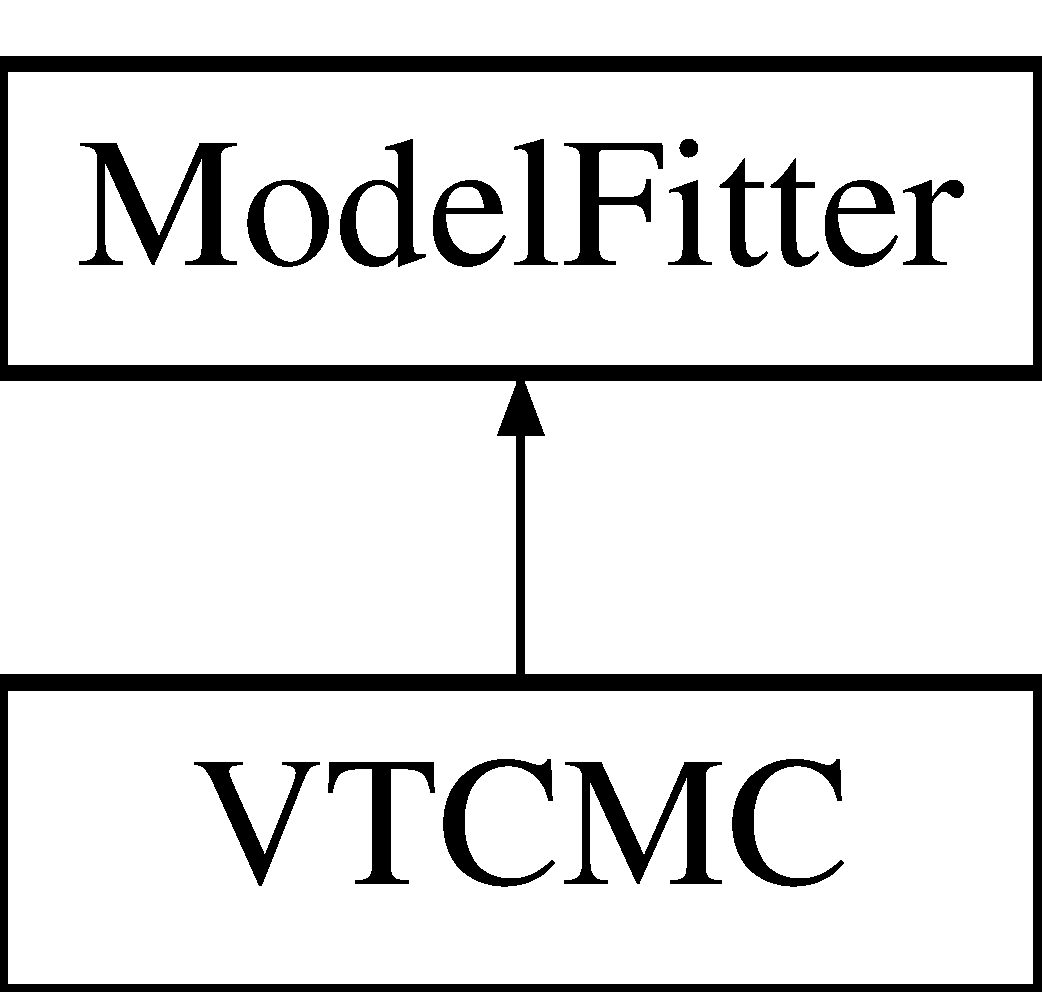
\includegraphics[height=2.000000cm]{classVTCMC}
\end{center}
\end{figure}
\subsection*{Public Member Functions}
\begin{DoxyCompactItemize}
\item 
\hypertarget{classVTCMC_a7cdc21d7325fa2fd95d6f59bcaa9377a}{int {\bfseries fit} (\hyperlink{classDataConsolidator}{Data\-Consolidator} $\ast$dc)}\label{classVTCMC_a7cdc21d7325fa2fd95d6f59bcaa9377a}

\item 
\hypertarget{classVTCMC_a151cc09b8883efd4d08bef2e5588d1fe}{void {\bfseries write\-Header} (File\-Writer $\ast$fp, const \hyperlink{classResult}{Result} \&site\-Info)}\label{classVTCMC_a151cc09b8883efd4d08bef2e5588d1fe}

\item 
\hypertarget{classVTCMC_aa8f82bde6bc4ac931cdb6964bb1b25ff}{void {\bfseries write\-Output} (File\-Writer $\ast$fp, const \hyperlink{classResult}{Result} \&site\-Info)}\label{classVTCMC_aa8f82bde6bc4ac931cdb6964bb1b25ff}

\item 
\hypertarget{classVTCMC_ac2f5aaabdd65cc4b22c254846f4a7a65}{void {\bfseries reset} ()}\label{classVTCMC_ac2f5aaabdd65cc4b22c254846f4a7a65}

\end{DoxyCompactItemize}
\subsection*{Additional Inherited Members}


The documentation for this class was generated from the following file\-:\begin{DoxyCompactItemize}
\item 
Model\-Fitter.\-h\end{DoxyCompactItemize}

\hypertarget{classWarningOnce}{\section{Warning\-Once Class Reference}
\label{classWarningOnce}\index{Warning\-Once@{Warning\-Once}}
}
\subsection*{Public Member Functions}
\begin{DoxyCompactItemize}
\item 
\hypertarget{classWarningOnce_a78ee7f515a6beb2be60c6507cebda978}{{\bfseries Warning\-Once} (const std\-::string \&msg)}\label{classWarningOnce_a78ee7f515a6beb2be60c6507cebda978}

\item 
\hypertarget{classWarningOnce_a1c38737eb932bc9f1dff13dc404a4352}{void {\bfseries warning\-If} (bool cond)}\label{classWarningOnce_a1c38737eb932bc9f1dff13dc404a4352}

\end{DoxyCompactItemize}


The documentation for this class was generated from the following file\-:\begin{DoxyCompactItemize}
\item 
Data\-Consolidator.\-h\end{DoxyCompactItemize}

\hypertarget{classZegginiTest}{\section{Zeggini\-Test Class Reference}
\label{classZegginiTest}\index{Zeggini\-Test@{Zeggini\-Test}}
}
Inheritance diagram for Zeggini\-Test\-:\begin{figure}[H]
\begin{center}
\leavevmode
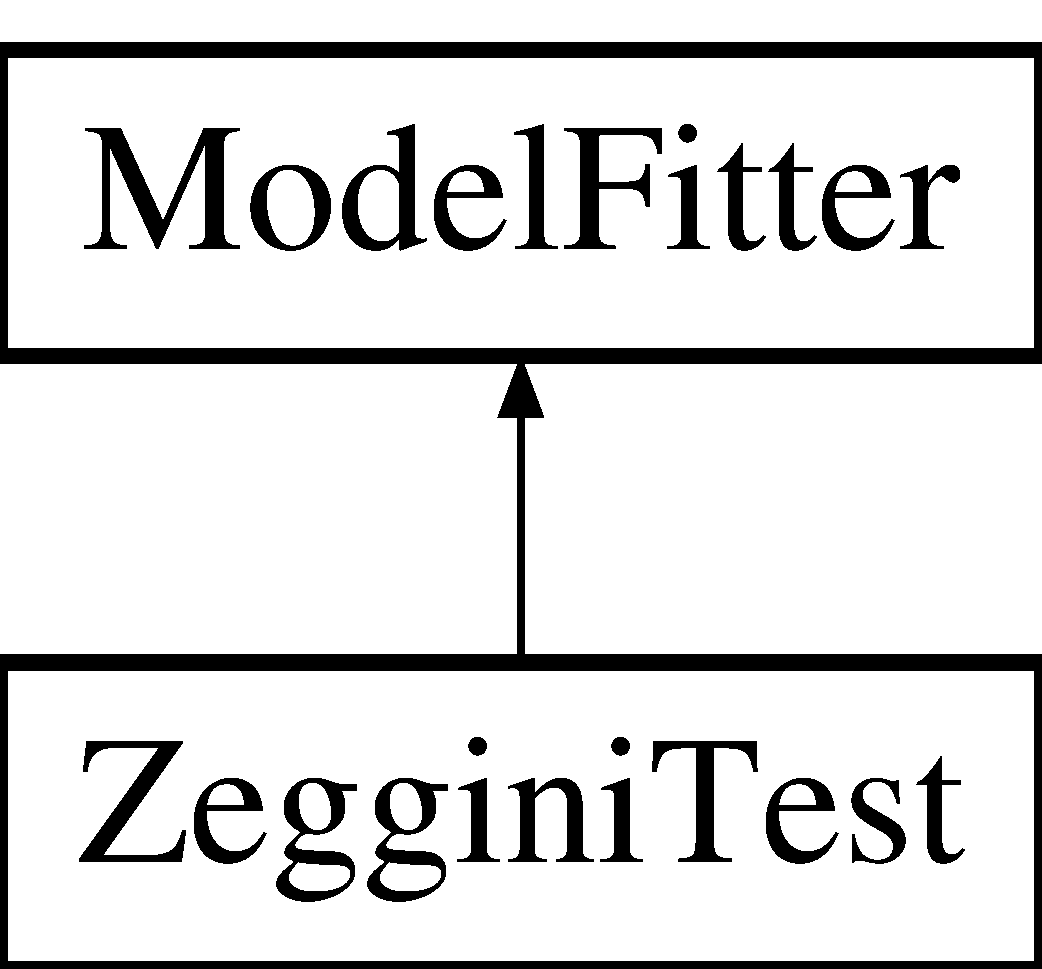
\includegraphics[height=2.000000cm]{classZegginiTest}
\end{center}
\end{figure}
\subsection*{Public Member Functions}
\begin{DoxyCompactItemize}
\item 
\hypertarget{classZegginiTest_abe558e2fc439c89b3ee6034b361ad8fe}{int {\bfseries fit} (\hyperlink{classDataConsolidator}{Data\-Consolidator} $\ast$dc)}\label{classZegginiTest_abe558e2fc439c89b3ee6034b361ad8fe}

\item 
\hypertarget{classZegginiTest_a47b8695cfc4b866c1d53611bb1f4a61f}{void {\bfseries write\-Header} (File\-Writer $\ast$fp, const \hyperlink{classResult}{Result} \&site\-Info)}\label{classZegginiTest_a47b8695cfc4b866c1d53611bb1f4a61f}

\item 
\hypertarget{classZegginiTest_aa2c9f4e741f4d4cfe91a652a8e2e277a}{void {\bfseries write\-Output} (File\-Writer $\ast$fp, const \hyperlink{classResult}{Result} \&site\-Info)}\label{classZegginiTest_aa2c9f4e741f4d4cfe91a652a8e2e277a}

\end{DoxyCompactItemize}
\subsection*{Additional Inherited Members}


The documentation for this class was generated from the following file\-:\begin{DoxyCompactItemize}
\item 
Model\-Fitter.\-h\end{DoxyCompactItemize}

\hypertarget{classZegginiWaldTest}{\section{Zeggini\-Wald\-Test Class Reference}
\label{classZegginiWaldTest}\index{Zeggini\-Wald\-Test@{Zeggini\-Wald\-Test}}
}
Inheritance diagram for Zeggini\-Wald\-Test\-:\begin{figure}[H]
\begin{center}
\leavevmode
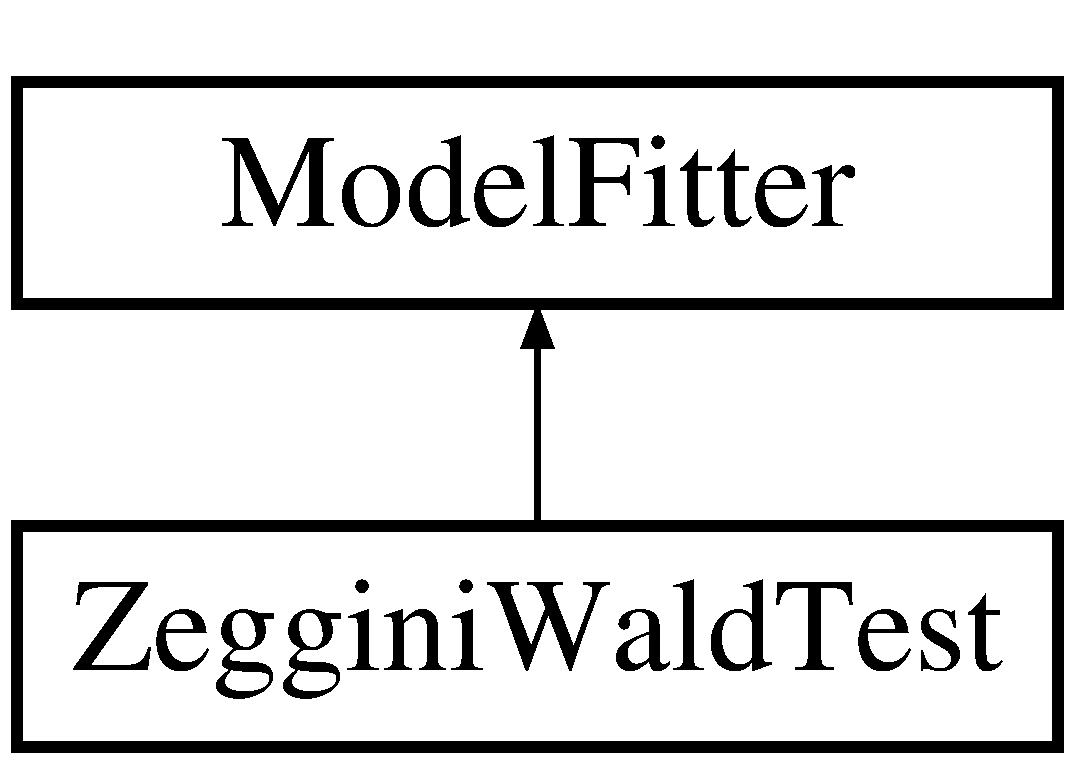
\includegraphics[height=2.000000cm]{classZegginiWaldTest}
\end{center}
\end{figure}
\subsection*{Public Member Functions}
\begin{DoxyCompactItemize}
\item 
\hypertarget{classZegginiWaldTest_ae91ad9cc600feeff2441223a543d23e1}{int {\bfseries fit} (\hyperlink{classDataConsolidator}{Data\-Consolidator} $\ast$dc)}\label{classZegginiWaldTest_ae91ad9cc600feeff2441223a543d23e1}

\item 
\hypertarget{classZegginiWaldTest_aa69d4617f52b3788b3eea25209d5a5e4}{void {\bfseries write\-Header} (File\-Writer $\ast$fp, const \hyperlink{classResult}{Result} \&site\-Info)}\label{classZegginiWaldTest_aa69d4617f52b3788b3eea25209d5a5e4}

\item 
\hypertarget{classZegginiWaldTest_a09cbc2b0cb9795567f79ae639d61c398}{void {\bfseries write\-Output} (File\-Writer $\ast$fp, const \hyperlink{classResult}{Result} \&site\-Info)}\label{classZegginiWaldTest_a09cbc2b0cb9795567f79ae639d61c398}

\end{DoxyCompactItemize}
\subsection*{Additional Inherited Members}


The documentation for this class was generated from the following file\-:\begin{DoxyCompactItemize}
\item 
Model\-Fitter.\-h\end{DoxyCompactItemize}

\printindex
\end{document}
